%\documentclass[sigconf, authordraft]{acmart}
\documentclass[sigconf, authordraft, anonymous]{acmart}
\usepackage{subcaption}
\usepackage{graphicx}
%\usepackage{fontspec} 
%\usepackage{polyglossia} 
%\setdefaultlanguage{english}
%\usepackage{xeCJK}
%\setCJKmainfont{Hiragino Mincho Pro}

%\usepackage[style=authoryear,%
%language=auto,%
%autolang=langname,%
%]{biblatex}

\usepackage{graphicx}
\usepackage{amsmath}
\usepackage{amssymb}
\usepackage{algorithm}
\usepackage[noend]{algpseudocode}
\usepackage{booktabs} % For formal tables

\usepackage{colortbl}

\definecolor{maroon}{cmyk}{0,0.87,0.68,0.32}

\newcommand{\gray}{\rowcolor[gray]{.90}}

% Copyright
%\setcopyright{none}
%\setcopyright{acmcopyright}
%\setcopyright{acmlicensed}
\setcopyright{rightsretained}
%\setcopyright{usgov}
%\setcopyright{usgovmixed}
%\setcopyright{cagov}
%\setcopyright{cagovmixed}


% DOI
\acmDOI{10.1145/nnnnnnn.nnnnnnn}

% ISBN
\acmISBN{978-x-xxxx-xxxx-x/YY/MM}

% Conference
\acmConference[GECCO '19]{the Genetic and Evolutionary Computation Conference 2019}{July 13--17, 2019}{Prague, Czech Republic}
\acmYear{2019}
\copyrightyear{2019}

%\acmArticle{4}
\acmPrice{15.00}

% These commands are optional
%\acmBooktitle{Transactions of the ACM Woodstock conference}
%\editor{Jennifer B. Sartor}
%\editor{Theo D'Hondt}
%\editor{Wolfgang De Meuter}


\begin{document}
%\title{MOEA/D - New Resource Allocation Functions Diversity Based}
\title{Using Diversity as a Priority Function for Resource Allocation on MOEA/D}
%\titlenote{Produces the permission block, and
%  copyright information}
%\subtitle{Subtitle}
%\subtitlenote{The full version of the author's guide is available as
%  \texttt{acmart.pdf} document}

%%% The submitted version for review should be ANONYMOUS
\author{Yuri Lavinas}
%\authornote{XXX}
\affiliation{%
	\institution{University of Tsukuba}
	\streetaddress{XXX}
	\city{Tsukuba} 
	\country{Japan}}
\email{yclavinas@gmail.com}

\author{Claus Aranha}
%\authornote{XXX}
\affiliation{%
	\institution{University of Tsukuba}
	\streetaddress{XXX}
	\city{Tsukuba} 
	\country{Japan}}
\email{caranha@cs.tsukuba.ac.jp}

\author{Testuya Sakurai}
%\authornote{XXX}
\affiliation{%
  \institution{University of Tsukuba}
  \streetaddress{XXX}
  \city{Tsukuba} 
  \country{Japan}}
\email{sakurai@cs.tsukuba.ac.jp}

% The default list of authors is too long for headers.
%\renewcommand{\shortauthors}{B. Trovato et al.}

%
\begin{abstract}
	Multi-objective Evolutionary Algorithm based on Decomposition, MOEA/D, decomposes multi-objective problems into single-objective subproblems. All subproblems are uniformly treated and there is no priority among them. Each subproblem is related to an area of the theoretical Pareto Front. It is expected that different areas would be more difficult to approximate than others, leading to an unbalanced exploration of the search space. To balance exploration, "Resource Allocation" techniques that prioritize certain subproblems were proposed. Here we investigate how priority functions relate to MOEA/D in terms of performance. We consider four different methods as priority functions: diversity on the objective space, diversity in the decision space, a priority function with random values and the relative improvement, from MOEA/D-DRA. We conducted an experimental analysis on the DTLZ and UF benchmark problems and on the lunar landing real-world problem and compared the famous MOEA/D-DE variant with each four priority functions and without any. The results indicate XXX.
\end{abstract}


%% The code below should be generated by the tool at
%% http://dl.acm.org/ccs.cfm
%% Please copy and paste the code instead of the example below. 
%%
%\begin{CCSXML}
%<ccs2012>
% <concept>
%  <concept_id>10010520.10010553.10010562</concept_id>
%  <concept_desc>Computer systems organization~Embedded systems</concept_desc>
%  <concept_significance>500</concept_significance>
% </concept>
% <concept>
%  <concept_id>10010520.10010575.10010755</concept_id>
%  <concept_desc>Computer systems organization~Redundancy</concept_desc>
%  <concept_significance>300</concept_significance>
% </concept>
% <concept>
%  <concept_id>10010520.10010553.10010554</concept_id>
%  <concept_desc>Computer systems organization~Robotics</concept_desc>
%  <concept_significance>100</concept_significance>
% </concept>
% <concept>
%  <concept_id>10003033.10003083.10003095</concept_id>
%  <concept_desc>Networks~Network reliability</concept_desc>
%  <concept_significance>100</concept_significance>
% </concept>
%</ccs2012>  
%\end{CCSXML}

%\ccsdesc[500]{Computer systems organization~Embedded systems}
%\ccsdesc[300]{Computer systems organization~Redundancy}
%\ccsdesc{Computer systems organization~Robotics}
%\ccsdesc[100]{Networks~Network reliability}
%

\keywords{ACM proceedings, \LaTeX, text tagging}

\maketitle

\section{Introduction}

% Define MOP
Multi-objective Optimization Problems (MOP) are maximization (or minimization)
problems characterized by multiple, conflicting objective functions. It arises
in real world applications that require a compromise among multiple objectives.
Thet of optimal trade off solutions in the decision space is the \emph{Pareto
Set}, and the image of this set in the objective space is the \emph{Pareto
Front}. Finding a good approximation of the Pareto Front is a hard problem for
which multiple Evolutionary Algorithms have been proposed.

% Mention that MOEAD is a good approach for MOP
The Multi-Objective Evolutionary Algorithm Based on Decomposition
(MOEA/D)~\cite{zhang2007moea} is an effective algorithm for solving MOPs. The
key idea of the MOEA/D is that the multi-objective optimization problem is
decomposed into a set of single objectives subproblems All subproblems
are then solved in parallel.

% Mention that MOEAD all problems are treated equally, but in actually they are
In the original MOEA/D, all subproblems are treated uniformly, in the sense that
all of them receive the same computational effort. However, it has been observed
that some subproblems are harder than others, and take more effort to converge
to an optimal solution~\cite{zhou2016all}. Because of this, \emph{Resource
Allocation} approaches have been proposed to allocate different amount of
computational effort to different subproblems, based on an estimation of the
relative difficulty of each subproblem~\cite{zhou2016all, zhang2009performance,
kang2018collaborative}. The most popular approach for estimating subproblem
difficulty is the Relative Improvement, which calculates how much a subproblem
has improved in recent iterations.

% Motivation for this approach
Here, we propose a new approach for estimating difficulty and
calculating priority in Resource Allocation for MOEA/D. Our approach uses the
idea of \emph{diversity} in decision space and in objective space to calculate
the priority of solutions. Our motivation for this choice is that the quality of
a MOP solution set is often evaluated by the diversity in the objective space.
If we assign higher priority for regions with lower diversity, we are
encouraging the algorithm to spend more computational effort in regions that are
not yet well explored.

% Simplify the paragraph below (important point is an outline of how we calculate diversity in both cases (In this paper, we define a priority function based on diversity using .........))
In this paper, we define a priority function based on diversity on the objective space using the MRDL, proposed by Gee~\ref{gee2015online}. The MRDL is an online diversity metric based on a geometrical perspective and indicates the loss of diversity related to a solution to the whole population. We also define a priority function based on diversity on the decision space using the 2-Norm. It compares solutions by measuring the norm of  the difference of these solutions. We understand that these priority functions are able to monitor diversity during the execution of the algorithm guiding the search behavior of the algorithm.


% Expand the paragraph below with more details on the results and conclusions
% Use the abstract as inspiration. 
We compare the new approach with the Relative Improvement or not using priority functions at all. The results show that focusing on diversity leads to better results on the metrics Hypervolume (HV) and Inverted Generational Distance (IGD) and also lead to a higher percentage of non-dominated solutions. The diversity on the decision space shows better performance on the benchmark function,  generally being better than using the relative improvement. It came to our surprise that the diversity on the objective space barely improve the results of not using priority functionsm in the artificial benchmarks. On the other hand, using diversity on the objective space as a priority function excels in the Lunar Landing problem.

%The results found supported that idea, since in the real-world Lunar Landing problem these priority functions performed very well (with emphasis on the results of the 2-Norm). In the UF benchmark problem only 2-Norm performed well, followed closely by the relative improvement. All code is available for reproducibility purpose.

% This balance is defined by the concept of ``pareto dominance''. Given two
% solutions vectors $u, v$ in $\mathbb{R}^{D}$, $u$  Pareto-dominates $v$, we
% say that denoted by $f(u) \prec f(v)$, if and only if $f_k(u) \leq f_k(v),
% \forall_k \in \{1,..., m\}$ and $ f(u) \neq f(v)$. Likewise, a solution $x \in
% \mathbb{R}^{D}$ is considered Pareto-Optimal if there exists no other solution
% $y \in \mathbb{R}^{D}$ such that $f(y) \succ f(x)$, i.e., if $x$ is
% non-dominated in the feasible decision space. A non-dominated solution exists
% if no other solution provides a better trade-off in all objectives.

% Consequently, the set of all Pareto-Optimal solutions is known as the Pareto-Optimal Set (PS), while the image of this set is referred to as the Pareto-optimal Front (PF).\\
% \vspace{-1em}
% \begin{equation}
% PS = \{x \in \mathbb{R}^{D} | \nexists y \in \mathbb{R}^{D} : f(y) \succ f(x)  \},
% \end{equation}
% \vspace{-1em}
% \begin{equation}
% PF = \{f(x) | x \in PS \}.
% \end{equation}

%Multi-objective evolutionary algorithms (MOEAs) are one of the most widely used groups of algorithms for finding approximations to the PF of a MOP. They are characterized by their ability to find good approximations to PF in a single run~\cite{zhou2011multiobjective}. In recent years, there has been an increasing interest in studying MOEAs and with a primary concern of improving their general performance.% Among MOEAs, there are three major paradigms: Pareto domination-based approaches~\cite{deb2002fast},~\cite{zitzler2001spea2}; indicator-based approaches~\cite{beume2007sms},~\cite{zitzler2004indicator} and decomposition-based approaches~\cite{li2009multiobjective},~\cite{zhang2007moea}.

%Multi-objective evolutionary algorithms (MOEAs) are one of the most widely used groups of algorithms for finding approximations to the PF of a MOP. They are characterized by their ability to find good approximations to PF in a single run~\cite{zhou2011multiobjective}. In recent years, there has been an increasing interest in studying MOEAs and with a primary concern of improving their general performance. Among MOEAs, there are three major paradigms: Pareto domination-based approaches~\cite{deb2002fast}; indicator-based approaches~\cite{beume2007sms}; and decomposition-based approaches~\cite{zhang2007moea}.

% We are interested in analyzing the Multi-objective Evolutionary Algorithm based on Decomposition framework, MOEA/D~\cite{zhang2007moea}. It represents a class of population-based meta-heuristics for solving Multi Objective Problems. In
% this framework, each individual has a specific weight vector which is used to decompose the original multi-objective problem into simpler, single-objective subproblems by means of scalarizations. Each subproblem is then evaluated and its utility value is calculated by an aggregation function given the related weight vector.

% In the original MOEA/D, each solution of a subproblem have the same amount of computational resource (number of iteractions). Each subproblem relates to a region of the PF. Since all of them are uniformly treated, it is expected that different regions of the would be more difficult to find approximations than other areas leading to an unbalanced exploration of the search space.
%\begin{figure}[h]
%	\centering
%	\includegraphics[width=0.55\textwidth]{img/decomp2.png}
%	\caption{A decomposition strategy generates weight vectors that defines the subproblems. Figure from~\cite{chugh2017handling}.}
%	\label{fig1}
%\end{figure}
%
%\begin{figure}[h]
%	\centering
%	\includegraphics[width=0.43\textwidth]{img/harder_problems}
%	\caption{Distribution of optimal solutions of subproblems with uniform weight vectors on ZDT3. Figure from~\cite{li2015use}.}
%	\label{fig2}
%\end{figure}
%
%
%\begin{figure}[h]
%	\centering
%	\includegraphics[width=0.53\textwidth]{img/harder_problems2}
%	\caption{An example that uniformly distributed weights may lead to different distributions of optimal solutions. (a) Solutions $s_1$ to $s_7$ are the optimal solutions of weights $w_1$ to $w_7$, respectively. (b) Solutions $s_1$,$s_2$,$s_3$,$s_6$ and $s_7$ are the optimal solutions of $w_1$,$w_2$,$w_3$,$w_6$ and $w_7$, respectively, while solution $s_5$ is the optimal solution of $w_4$ and $w_5$.Figure from~\cite{li2017weights}}
%	\label{fig3}
%\end{figure}


%
%Another way, is allocating different number of evaluations to the subproblems based on some priority function. In a few recent works, a priority function (also called utility function) is used to prioritize resources given to subproblems that contribute more to the algorithm's search.  In the works of Zhang et al.~\cite{zhang2009performance} and Zhou et al.~\cite{zhou2016all} a priority function was proposed aiming to prioritize solutions based on a historical convergence information during different generations. Another approach was implemented in Kang et al.~\cite{kang2018collaborative}, where the priority function was based on the presence of a solution from the main population on a secondary population.

% Although researchers have not studied this problem in much detail, there have been some works that have discussed this matter. One way to address this problem is to allocate different number of evaluations to the subproblems based on some priority function. In a few recent works, a priority function (also called utility function) is used to prioritize resources given to subproblems that contribute more to the algorithm's search.  In the works of Zhang et al.~\cite{zhang2009performance} and Zhou et al.~\cite{zhou2016all} a priority function was proposed to prioritize solutions based on convergence information during different generations. Another approach was implemented in Kang et al.~\cite{kang2018collaborative}, where the priority function was based on the presence of a solution from the main population on a secondary population.

\section{Background}

\subsection{Priority functions}

%Following the discussion opened in the introduction, we need to define an utility function to allocate the number of evaluations to subproblems. 
We define priority functions (also called utility functions) as one way of establishing preferences~\cite{chankong1983multiobjective} between solutions for resource allocation. These functions are used to decide how to allocate computational resources among subproblems by monitoring the algorithm search and guiding the distribution over generations~\cite{cai2015external}. 

Only a few studies have been concerned with resource allocation. We highlight two groups. The first is composed by MOEA/D-GRA~\cite{zhou2016all}, MOEA/D-DRA~\cite{zhang2009performance} and in the Two-Level Stable Matching-Based Selection in MOEA/D~\cite{nasir2011improved}. The other is composed by EAG-MOEA/D~\cite{cai2015external} and MOEA/D-CRA~\cite{kang2018collaborative}.

According to Zhou and Zhang~\cite{zhou2016all}, MOEA/D-GRA may be seen as an extension of MOEA/D-DRA and MOEA/D-AMS~\cite{chiang2011moea}. They reason that all these algorithms use a very similar priority function and that MOEA/D-GRA can simulate the behavior of MOEA/D-DRA or MOEA/D-AMS by changing the values of a single parameter. 

This priority function is named as the relative improvement (R.I.) and defines the priority values of each subproblem $i=1,...,N$, as

\begin{equation}\label{priority}
	\delta_i = \dfrac{\text{old function value}-\text{new function value}}{\text{old function value}}.
\end{equation}

For MOEA/D-GRA $u_i = \delta_i$, but in MOEA/D-DRA, as well as in the Two-Level Stable Matching-Based Selection in MOEA/D, a second equation is used,

\[
u_i= 
\begin{cases}

(0.95 + 0.05 \cdot \frac{\delta_i}{0.001} \cdot u_i), & \text{if } \delta_i > 0.001,
\\
1,              & \text{otherwise}

\end{cases}\label{priority2}
\]
The R.I. is based the assumption that if a subproblem has been improved over the last $\Delta T$ generations (\textit{old function value}), it should have a high probability of being improved over the next generations. 
	
The priority function used EAG-MOEA/D~\cite{cai2015external} and MOEA/D-CRA~\cite{kang2018collaborative} differ from the ones in the MOEA/D-GRA group. In their case, the framework keeps two populations: one working population, and one external archive. This priority function estimates priorities for a subproblem given the number of solutions from that subproblem that are in the external archive.

Together these studies indicate that it is worth monitoring the algorithm behavior and guiding its search, but it is unclear how the priority functions influence into the results since in all the impact of using priority functions was not isolated. That is, in all of the work previously mentioned incremented MOEA/D with priority functions and at least an extra. For example, in Zhang et al. used a 10-tournament selection in MOEA/D-DRA~\cite{zhang2009performance}, while Zhou and Zhang used a new replacement strategy in MOEA/D-GRA~\cite{zhou2016all}. Chiang in MOEA/D-AMS proposes an adaptive mating selection mechanism as dynamically adjusts the mating pools of individuals~\cite{chiang2011moea}. Finally, both the studies of Cai and Lai in  EAG-MOEA/D~\cite{cai2015external} and Kang et al. in MOEA/D-CRA~\cite{kang2018collaborative} used an archive population.

Based on the recent success of addressing resource allocation with priority functions, we aim to isolate priority functions by analyzing their impact in MOEA/D. In this study we propose two new priority functions to further understand how priority functions influence the performance of MOEA/D framework. We believe in the idea that diversity is a critical issues of a search process in any multi-objective algorithm. Therefore, we consider using priority functions to address lack of diversity aiming to make solutions better spread among each other and proposed two new priority functions. 

These two priority functions focus on different aspects of the diversity:  how to better spread solutions along the PF (diversity on the objective space) by using the MRDL and how to better spread solutions the PS (diversity on the decision space) by using the Norm of the difference between two solutions.



\subsection{Diversity Metric}


Over the last two decades, some works in diversity metrics have been successfully applied in different tasks on evolutionary computation. One way to measure diversity is to use metrics that evaluate MOPs solvers. The hypervolume indicator (HV)~\cite{zitzler1998multiobjective} and the Inverted Generational Distance (IGD)~\cite{zhang2008rm} are frequently used as metrics to evaluate such solvers. However they include information about both quality of the solutions and diversity in a single metric.

Among the metrics that only measure diversity, we highlight those that calculate the diversity during the execution of the algorithm. Those are: the sigma method~\cite{mostaghim2003strategies} that requires that the PF lies in the positive objective space; measurement of the entropy of solutions by using Parzen window density estimation-\cite{tan2008evolutionary}, that is sensitive to kernel width; and the maximum relative diversity loss, MRDL, ~\cite{gee2015online}, a very expensive method - $O(N^2)$, $N$ being the size of the parent population.


%Among the metrics that only measure diversity, there are mainly two groups. The offline group, that calculate the diversity after the execution of the algorithm, while online group, that calculate the diversity during the execution of the algorithm. We are interested in measuring diversity during the execution of the algorithm, therefore we  briefly introduce some studies that are part of the online group.
%
% The offline group is composed of: Chi-square-like deviation~\cite{deb1989genetic}; Spacing method~\cite{scott1995fault}; Uniformly distribution index~\cite{tan2002evolutionary}; Entropy approach~\cite{farhang2002diversity}; Grid diversity metric~\cite{deb2002running}; sparsity measure~\cite{deb2003fast}. These published studies need knowledge of the PF or the ideal vector. While the online group is composed of: sigma method~\cite{mostaghim2003strategies}  (PF lies in the positive objective space); entropy of the solutions by using Parzen window density estimation-\cite{tan2008evolutionary} (sensitive to kernel width); maximum relative diversity loss~\cite{gee2015online} (expensive $O(N^2)$, with $N$ being the size of the parent population).

In this work we chose to apply the MRDL as the strategy to measure diversity on the objective space. This is an online diversity metric estimates the diversity loss of a solution to the whole population~\cite{gee2015online}. High values indicate the existence of similar solutions or that the offspring solution is close to the convergence direction. The further an objective vector of a solution is from the convergence direction, the more it contributes for the diversity of the approximated the Pareto front. The MRDL is the maximum value for Relative Diversity Loss (RDL) of each solution.

To deal with diversity on the decision space we consider the similarity of decision vectors of consecutive iteractions given by the (2-)Norm. The Norm is defined similarly as the R.I., since in both a difference between vectors values from distinct iteractions. However there are two main differences between R.I. and Norm priority function. The first is that while the R.I. considers the function values of solutions the Norm considers its decision values. The second difference is that R.I. also considers equation~\ref{priority2}.
\section{MOEA/D with priority Functions}

%MOEA/D-RAD, MOEA/D with online Resource Allocation by Diversity Metric, is the variant of MOEA/D proposed in this work. This algorithm uses the maximum relative diversity loss, MRDL, for determining the values of the priority function. 


\begin{algorithm}[h]
	\caption{MOEA/D with priority functions}\label{alg1}
	\begin{algorithmic}[1]
		
		\State Initialize the weight vectors $\lambda_i$, the neighborhood $B_i$, the priority value $u_i$ every subproblem $i=1,...,N$.
		
		\While{\textit{Termination criteria}}
		\For {1 to N}
		\If{$\textit{rand()} < u_i$}
		\State Generate an offspring $y$ for subproblem $i$.
		\State Update the population by $y$.
		\EndIf
		\EndFor
		\State  Evaluate and after $\Delta T$ generations, keep updating \textit{\textbf{u}} by a priority function.
		\EndWhile
	\end{algorithmic}
	%\vspace{-1em}
\end{algorithm}

In this study we use the basic algorithm framework~\ref{alg1}with priority functions of MOEA/D-GRA. In contrast to  MOEA/D-GRA we only consider the basic algorithm and no other variant. The benefit of using MOEA/D-GRA is that it has a simple code structure and represents well the class of variants of MOEA/D with resource allocation. Therefore, our new functions based on diversity are then easily integrated to the MOEA/D framework.Except for line 4, in which a subproblem may not be part of the group that is going to be iterated and for line 7, in which the priority function is calculated, the whole procedure is similar to the MOEA/D-DE~\cite{zhang2009performance}. All reproduction procedures and parameters are the same as in MOEA/D-DE~\cite{li2009multiobjective}. We highlight that the neighborhood is only calculated in the initialization period.



%The update procedure is described The algorithm~\ref{alg2}, as in MOEA/D-GRA~\cite{zhou2016all}.
The decomposition method used is the Simple-Lattice Design (SLD), the scalar aggregation function used is Weighted Sum (WS), the update strategy used is the Restricted update strategy and we performed a simple linear scaling of the objectives to [0, 1].


%\subsection{Priority Functions}

We understand that priority functions provides an important property. It provides ways of designing MOEA/D variants that could focus on a desired characteristics, such as diversity, performance contribution, convergence to a specific region of the PF or others. This is possible because different methods can be used as priority functions to create the vector $u$ in algorithm~\ref{alg1}. 

In this work we chose to focus on studying four different characteristics: diversity on the objective space, diversity in the decision space, no information (random values) and the relative improvement, from MOEA/D-DRA as our priority functions. Next we give a brief explanation of why we chose to consider these  our methods and we describe the details of how to calculate them.

Independently of the method used to calculate the priority function, we initialize the value of the vector $u=1$, as in MOEA/D-DRA. As in DRA and GRA we have a learning period, $\Delta T$ generations (\textit{old function value}). Here $\Delta T=20$ for artificial benchmarks, as in MOEA/D-GRA~\cite{zhou2016all}, while for the real-world problems, we chose $\Delta T=2$, by trial and error. A sensitivity analyzes should be performed for deciding suitable initial values for $u$ and for $\Delta T$.

 It should also be noticed that once less than $3$ or less subproblems would be improved in a given iteraction $i$, we reset the priority vector $u = 1$  and all subproblems will be chosen for offspring reproduction at the that $i$ iteraction.

\subsection{Priority Function - Norm of the difference of current solutions and its parents} 

\begin{algorithm}[t]
	\caption{2-Norm}\label{alg3}
	\begin{algorithmic}[1]
		
		\State Input: NEW new incumbent solutions; OLD, previous iteraction incumbent solutions; N, the population size.
		\For {i=1 to N} 
			\State u[i] = $||$New[i] - OLD[i]$||$
		\EndFor
		\State u = scale (u) // between 0 and 1\\
	\Return u
	\end{algorithmic}
\end{algorithm}

The priority function proposed that considers diversity on the objective space is based on the 2-Norm,

\begin{equation}
 \text{2 Norm}_i = ||\text{current solution} - \text{parent solution}||.
\end{equation}

The idea of the 2-Norm as priority function is that by using diversity on decision space as the priority function more resources are given to incumbent solutions that are similar. Hence more effort is used focusing on modifying solutions that are close in the decision space, leading to a higher exploration of the decision space.


\subsection{Priority Function - MRDL} 


\begin{algorithm}[t]
	\caption{MRDL}\label{alg2}
	\begin{algorithmic}[1]
		
		\State Input: old MRDL (initial value is 0); C, objective function values from the incumbent solutions; P, objective function values from the previous iteraction incumbent solutions; N, the population size.
		\For {i=1 to $|C|$}
		\State find $h \in |P|$ where  ($P_h \succeq C_i$) and $||P_h - C_i  ||$ is minimal.
		\State $d.conv_{y} = C_i - P_h$.
		\For {j=1 to N}
		\State $p = P_j - P_h$
		\State $c = c_j - c_i$
		\State $proj_{d.conv_{y}}*p \prime = \dfrac{sum(conv_{y} \cdot p \prime)}{(p \prime \times p \prime)}*p \prime$
		
		\State $ proj_{d.conv_{y}}*c \prime = \dfrac{sum(conv_{y} \cdot c \prime)}{(c \prime \times c \prime)}*c \prime$
		
		\State $RDL = \dfrac{ ||p \prime - proj_{d.conv_{y}}p \prime|| }{||c \prime - proj_{d.conv_{y}}c \prime||}            $
		\EndFor
		MDRL[i] = maximum RDL
		\EndFor
		\State u = 1 - scale (MRDL - old MRDL) // between 0 and 1\\
	\Return u, MRDL
	\end{algorithmic}
\end{algorithm}


The diversity on objective space as a priority function  is based on the Maximum Relative Diversity Loss, MRDL~\cite{gee2015online}.  The idea using MRDL as a priority function is that by measuring diversity on the objective space, more resources are given to incumbent solutions that have similar objective function values between two consecutive iteractions leading to a higher exploration of the objective space. Algorithm~\ref{alg2} gives the details on implementation.
 
Now, we move on how to calculate MRDL. Prior to scalarizing it between $0$ and $1$ to fit the algorithm~\ref{alg1} we calculate MRDL for every individual of the population. The following equation describes how to calculate the priority function given the MRDL, $\Gamma^{p \rightarrow c}$.


\vspace{-1em}
\begin{equation}
\Gamma_{i}^{p \rightarrow c} = \underset{i=1,...,k}{\max} \Gamma_{d.conv_{y}}^{p \rightarrow c}.
\end{equation}



At every iteraction and for each incumbent solution, we need $k$ convergence directions (shown later) and we compute the Relative Diversity Loss (RDL) for each of these $k$ convergence directions. The maximum value among these $k$ convergence directions is chosen as the MRDL for that incumbent solution.

\begin{equation}
\label{rdl}
\Gamma_{d.conv_{y}}^{p \rightarrow c} = \dfrac{ ||p \prime - proj_{d.conv_{y}}p \prime|| }{||c \prime - proj_{d.conv_{y}}c \prime||}.
\end{equation}

To calculate RDL of a solution to the whole population, the following equation is used. It considers every incumbent solution related to a subproblem $i$, from the whole population. This reduction is given by a division between the shortest distance of a parent, $p$,  and offspring, $c$, to the line of convergence direction

%The numerator in~\ref{rdl} is the closest distance between the parent solution ($p$) to the convergence direction $(c_r - p_r)$. While, the denominator in~\ref{rdl} is the closest distance between the offspring solution ($c$) to the convergence direction $(c_r - p_r)$. %The projections of $p\prime$ and $c\prime$ objective vectors onto the convergence direction $d.conv_{y}$ are $proj_{d.conv_{y}}p \prime$ and $proj_{d.conv_{y}}c \prime$.

$p\prime$ and $c\prime $ are given by:
\vspace{-1em}
\begin{equation}
\begin{split}
p\prime = p - p_r,\\
c\prime = c - c_s,\\
\end{split}
\end{equation}
%verify this

with $p_r$ and $c_s$ being the parent, and offspring objective vectors used to calculate the convergence direction in equation~\ref{1}. Index $s$ is equal to index $j$ used to calculate $conv_{y}$. The same principle is valid for index $r$. The vector projection between two vectors is defined as next.

\begin{multline}
proj_{d.conv_{y}}p \prime = \frac {{d.conv_{y}} \cdot {p \prime}} {(p \times p)^2}{{p \prime}},\\
proj_{d.conv_{y}}c \prime = \frac {{d.conv_{y}} \cdot {c \prime}} {(c \times c)^2}{{c \prime}}.
\end{multline}

While the norm of $p \prime - proj_{d.conv_{y}}p \prime$ is calculated as follows using the 2-Norm of this difference. The same procedure is done for $c \prime - proj_{d.conv_{y}}c \prime$.

To estimate the convergence direction, $d.conv_{y}$, we need to have an offspring, $c_j$, that dominates at least one parent. Select a parent, $p_h$, solution that is closest to this offspring in the objective space.  For every weakly dominated parent, one convergence direction is calculated as in the next equation. As in the study by Zitzler et al.~\cite{zitzler2003performance} study, weak dominance ($A \succeq B$) means that any solution in set B is weakly dominated by a solution in set A. However, this does not rule out equality, because $A \succeq A$ for all approximation sets $A$.
\begin{equation}
\label{1}
d.conv_{y} = c_j - p_h
\end{equation}

Index $j$ (for indexing offsprings, $c_j$) is selected from the set $D_c$. Index $h$ is explained later.

\vspace{-1em}
\begin{equation}
\label{D}
D_c = \{d| \exists c_d \prec p_k, k \in {1,..., N}, d \in [1,..., |C|]\}
z\end{equation}

$N$ is the parent population size, $|C|$ is the size of the offspring population $C$. In equation~\ref{D}, the offspring $c_d$ must weakly dominate at least one parent solution. Index $h$ (for indexing parents, $p_h$) comes from the following two equations.
\begin{equation}
h = \underset{k \in D_p }{argmin} || p_k - c_j ||
\end{equation}

\begin{equation}
\label{D_p}
D_p = \{k| \exists c_j \prec p_k, k \in {1,..., N}\}
\end{equation}

$D_p$ in equation~\ref{D_p} denotes the index set of parent solutions which are weakly dominated by $c_j$ ($j$ index comes from equation~\ref{D}).



\subsection{Priority Function - Relative Improvement}  

\begin{algorithm}[t]
	\caption{Relative Improvement}\label{alg5}
	\begin{algorithmic}[1]
		
		\State Input:  C, objective function values from the incumbent solutions; P, objective function values from the $\Delta T$ previous iteraction incumbent solutions; N, the population size.
		\For {i=1 to N}
		\State u[i] = (C[i] - P[i])/C[i]
		\EndFor
		u / (max(u) + $1.0 x 10^{-50}$)\\
		\Return u
	\end{algorithmic}
\end{algorithm}

Here we give a brief description of the Relative Improvement (R.I.), the priority function used in MOEA/D-DRA, MOEA/D-GRA and many others. This priority function aims to measure subproblem hardness and then it helps allocating more resource to subproblems that have  improved more over the next few generations. Algorithm~\ref{alg5} gives the details on implementation of the equation~\ref{priority}. R.I. was first introduced in the context of the unconstrained MOEA competition in the CEC 2009~\cite{zhang2009performance}, being the winner of that competition~\cite{zhang2008multiobjective}. This competition also introduced the UF benchmark functions.

\subsection{Priority Function - Random}

\begin{algorithm}[t]
	\caption{Random}\label{alg4}
	\begin{algorithmic}[1]
		
		\State Input:  N, the population size.
		\For {i=1 to N}
		\State u[i] = random value between 0 and 1
		\EndFor
		\Return u
	\end{algorithmic}
\end{algorithm}

Finally, we describe the last priority function studied in this work. The random priority function is used a base for comparison. Given no information besides the size of the population, we define the vector of priority $u$ at random. Algorithm~\ref{alg4} gives the details on implementation. 
%
%
%
%Does is help? When we consider more sophisticated priority functions, are we making any improvement?
%
% Using no information. We select solutions at random.
% 
% if it is best
%
%bigger population might be worse, since if a subpopulation better results were found - to much effort for nothing
%smaller population might be better, since if a subpopulation better results were found - effort resource better spent
%subpopulation from a bigger population is better than smaller population with the subpopulation size?





\section{Experimental Design}

%\begin{table}[!t]
%	\centering
%\begin{tabular}{@{}|l|l|@{}}
%		\toprule
%		\textbf{Parameters}   & \textbf{Values}          \\ \midrule
%		Initial value $u$     & 0.5, for every subproblem \\ 
%		Population size       & 150                      \\
%		Neighborhood size T & 20 \\ 
%		$\delta_p$ & 0.9 \\ 
%		$\phi$ & 0.5 \\ 
%		$\eta_m$ & 20 \\
%		$p_m$ & 0.03333333 \\
%		$n_r$ & 2 \\
%		\midrule
%		Number of evaluations & 60000 		\\		
%		Number of repetitions & 21                  \\ \bottomrule
%
%	\end{tabular}
%\vspace{1em}
%\caption{Parameter settings.}
%\label{table1}
%\end{table}


The question that we want to answer is how MOEA/D-DE performs when combined with: no priority function (none) and the priority functions 2-norm, MRDL, relative improvement and random. To answer that question we apply MOEA/-DE with the 4 priority functions to two artificial benchmark problems and the Lunar Landing real-world problem and we compared the performance against the results of the MOEA/D-DE. We compared the variants of priority functions using the DTLZ benchmark functions from~\cite{deb2005scalable} with 100 dimensions and $k =$ dimensions - number of objectives $+ 1$, where the number of objectives is $2$. We also consider the UF benchmark functions from~\cite{zhang2008multiobjective}, also with 100 dimensions. 


%\subsubsection{Real World Benchmark Function}


The Lunar Landing problem is a real-world problem that simulates the selection of landing sites for lunar landers~\citep{MoonOrbitingSatellite2015}. In lunar exploration plan, finding suitable landing site of the rovers has a very important function. Good landing sites ensure enough sunshine to provide energy for the rovers power supply while being in a region with scientifically interesting materials with little difficulties to the exploration. This is a minimization problem in which the two decision variables are the longitude and latitude with the objectives being: the number of continuous shade days, the total communication time (in reality, this is a maximization problem that was inverted with the goal of consistency), and the inclination angles. Although the number of design variables is small as two (latitude and longitude), it is considered to be a severe constrained problem due to the presence of two craters. In values, the two constraints are defined as continuous shade days being $ < 0.05$ while inclination angles being $<0.3$

%\subsubsection{Parameter Settings}
For every combination, the parameters are as follows. The population size $N = 350$, the update size $nr = 2$, the neighborhood size $T = 20$, and the neighborhood search probability $\delta_p = 0.9$. The DE mutation operator value is $phi=0.5$. The Polynomial mutation operator values are $\eta_m 20$ and $p_m = 0.03333333$~\cite{campelo2018moeadr}. The number of executions is 21. At each execution, the number of functions evaluations is 70000. For the Lunar Landing, we highlight that differ from the settings for the artificial benchmarks. Since this problems is a severe constrained one, we chose the population size $N = 5050$ and the number of functions evaluations is 60000. 

We perform statistical tests on the hypervolume (HV) metric values and Inverted Generational Distance (IGD) for measuring the quality of a set of obtained non-dominated solutions found by the algorithms on the, DTLZ and UF benchmark problem. Before calculating the HV value, the objective function was scaled between $0$ and $1$. The reference point for the HV calculation was set to $(1, 1)$. For the real-world Lunar Landing problem, we only perform statistical tests on the hypervolume (HV) metric values and the reference point for the HV calculation was set to $(1, 0, 1)$. Higher values of the HV indicate better approximations while lower values of the IGD indicate better approximations. In order to verify any statistical difference in the average performance given the different algorithms, the Pairwise Wilcoxon Rank Sum Tests was used, with confidence interval $\alpha = 0.05$ and with the Hommel adjustment method. For reproducibility the code is made available at XXX.


\section{Results}

% We show images from the UF9 and DTLZ4 functions due to space limitations, but similar images for the other problems are available in the supplementary materials.

% Ideias para resultados
%%% In terms of IGD and HV, we can seee that in general, using resource allocation performs better than not using resource allocation. RI and Norm achieve similar results, and Random as well for HV, (but not IGD). These results are indicated by the boxplot, the tables, the pareto front, and the willcoxon pairwise analysis. For the Moon Landing problem, all strategies found similar Hypervolume results.

%%% The fact that random performed as well as Norm and RI in HV indicates that there is still space for finding more appropriate priority functions?

%%% Figure 4 shows how the different strategies are allocating results for functions UF9 and DTLZ4. It is interesting to observe that RI and Norm assign similar priorities to the same subproblems in the DTLZ4. But they find opposite priorities to subproblems on the UF9 function.

%%% Dominance and feasibility
% Another difference that we see among the Resource Allocation strategies is found in the proportion of non dominated and feasible solutions. For the Benchmark problems, the Norm Strategy achieved a very high fraction of non-dominated solutions in the final solution set. In the Lunar Landing problem, the Norm strategy achieved a higher proportion of feasible solutions than the other resource allocation strategies.





\begin{table*}[!t]
	\begin{tabular}{llllll}
		\cline{6-6}
		\hline
		\rowcolor[gray]{.7} \multicolumn{1}{|l|}{HV}         & \multicolumn{1}{l|}{None} & \multicolumn{1}{l|}{MRDL} & \multicolumn{1}{l|}{Norm} & \multicolumn{1}{l|}{R.I.} & \multicolumn{1}{l|}{Random} \\ \hline \hline  \hline
		\multicolumn{1}{l}{Lunar}           & \multicolumn{1}{l}{0.656 (0.034)} & \multicolumn{1}{l}{\textbf{0.687 (0.057)}} & \multicolumn{1}{l}{0.666 (0.060)} & 0.683 (0.067)             &\multicolumn{1}{l} {0.664 (0.047)} \\ \hline \hline \hline
		\rowcolor[gray]{.95} \multicolumn{1}{l}{UF1}              & \multicolumn{1}{l}{0.861 (0.011)} & \multicolumn{1}{l}{0.863 (0.015)} & \multicolumn{1}{l}{0.833 (0.022)} & \textbf{0.88 (0.013)}             &\multicolumn{1}{l} {0.874 (0.015)} \\ %\hline \hline
		\multicolumn{1}{l}{UF2}              & \multicolumn{1}{l}{0.750 (0.009)} & \multicolumn{1}{l}{0.750 (0.005)} & \multicolumn{1}{l}{ 0.762 (0.010)} & 0.82 (0.008)             &\multicolumn{1}{l} {\textbf{0.83 (0.008)}} \\ %\hline \hline
		\rowcolor[gray]{.95}\multicolumn{1}{l}{UF3}              & \multicolumn{1}{l}{0.844 (0.044)} & \multicolumn{1}{l}{0.860 (0.043)} & \multicolumn{1}{l}{ \textbf{0.944 (0.018)}} & 0.918 (0.029)             &\multicolumn{1}{l}  {0.909 (0.037)} \\ %\hline \hline
		\multicolumn{1}{l}{UF4}              & \multicolumn{1}{l}{0.364 (0.005)} & \multicolumn{1}{l}{0.366 (0.003)} & \multicolumn{1}{l}{ 0.372 (0.003)} & 0.371 (0.004)             &\multicolumn{1}{l} {\textbf{0.373 (0.004)}} \\ %\hline \hline
		\rowcolor[gray]{.95}\multicolumn{1}{l}{UF5}              & \multicolumn{1}{l}{0.629 (0.022)} & \multicolumn{1}{l}{0.663 (0.024)} & \multicolumn{1}{l}{ 0.754 (0.034)} & \textbf{0.811 (0.015)}             &\multicolumn{1}{l} {0.810 (0.016)} \\ %\hline \hline
		\multicolumn{1}{l}{UF6}              & \multicolumn{1}{l}{0.661 (0.020)} & \multicolumn{1}{l}{0.660 (0.014)} & \multicolumn{1}{l}{ 0.662 (0.020)} & 0.686 (0.014)             &\multicolumn{1}{l} {\textbf{0.689 (0.015)}} \\ %\hline \hline
		\rowcolor[gray]{.95}\multicolumn{1}{l}{UF7}              & \multicolumn{1}{l}{0.803 (0.010)} & \multicolumn{1}{l}{0.801 (0.010)} & \multicolumn{1}{l}{ 0.818 (0.012)} & \textbf{0.837 (0.005)}             &\multicolumn{1}{l} {0.834 (0.006)} \\ %\hline \hline
		\multicolumn{1}{l}{UF8}              & \multicolumn{1}{l}{0.894 (0.004)} & \multicolumn{1}{l}{0.900 (0.004)} & \multicolumn{1}{l}{ 0.914 (0.005)} & \textbf{0.922 (0.003)}             &\multicolumn{1}{l} {0.916 (0.004)} \\ %\hline \hline
		\rowcolor[gray]{.95}\multicolumn{1}{l}{UF9}              & \multicolumn{1}{l}{0.931 (0.004)} & \multicolumn{1}{l}{0.932 (0.004)} & \multicolumn{1}{l}{ \textbf{0.944 (0.014)}} & 0.932 (0.004)             &\multicolumn{1}{l} {0.940 (0.008)} \\ %\hline \hline
		\multicolumn{1}{l}{UF10}              & \multicolumn{1}{l}{0860 (0.017)} & \multicolumn{1}{l}{0.786 (0.017)} & \multicolumn{1}{l}{ 0.835 (0.035)} & \textbf{0.861 (0.033)}             &\multicolumn{1}{l} {0.839 (0.026)} \\ \hline  \hline \hline
		\rowcolor[gray]{.95}\multicolumn{1}{l}{DTLZ1}              & \multicolumn{1}{l}{0.989 (0.003)} & \multicolumn{1}{l}{0.991 (0.004)} & \multicolumn{1}{l}{ 0.997 (0.002)} & 0.998 (0.002)             & \multicolumn{1}{l} {\textbf{0.998 (0.001)}} \\ %\hline \hline
		\multicolumn{1}{l}{DTLZ2}              & \multicolumn{1}{l}{0.910 (0.002)} & \multicolumn{1}{l}{0.912 (0.002)} & \multicolumn{1}{l}{ \textbf{0.922 (0.001)}} & 0.921 (0.001)             & \multicolumn{1}{l} {\textbf{0.922 (0.001)}} \\ %\hline  \hline
		\rowcolor[gray]{.95}\multicolumn{1}{l}{DTLZ3}              & \multicolumn{1}{l}{0.960 (0.015)} & \multicolumn{1}{l}{0.969 (0.016)} & \multicolumn{1}{l}{ 0.992 (0.009)} &0.991 (0.009)             & \multicolumn{1}{l} {\textbf{0.993 (0.006)}} \\ %\hline \hline
		\multicolumn{1}{l}{DTLZ4}              & \multicolumn{1}{l}{0.905 (0.003)} & \multicolumn{1}{l}{0.907 (0.004)} & \multicolumn{1}{l}{0.920 (0.001)} &  \textbf{0.921 (0.004) }            & \multicolumn{1}{l} {0.918 (0.002)} \\ %\hline  \hline
		\rowcolor[gray]{.95}\multicolumn{1}{l}{DTLZ5}              & \multicolumn{1}{l}{0.895 (0.003)} & \multicolumn{1}{l}{0.898 (0.002)} & \multicolumn{1}{l}{ \textbf{0.910 (0.001)} }&0.908 (0.002)             & \multicolumn{1}{l} {\textbf{0.910 (0.001)}} \\ %\hline \hline
		\multicolumn{1}{l}{DTLZ6}              & \multicolumn{1}{l}{0.837 (0.035)} & \multicolumn{1}{l}{0.860 (0.021)} & \multicolumn{1}{l}{ \textbf{0.999 ($>$0.000)}} & 0.999 (0.001)             & \multicolumn{1}{l} {0.999 (0.001)} \\ %\hline  \hline
		\rowcolor[gray]{.95}\multicolumn{1}{l}{DTLZ7}              & \multicolumn{1}{l}{0.325 (0.056)} & \multicolumn{1}{l}{0.339 (0.048)} & \multicolumn{1}{l}{ \textbf{0.688 (0.005)}} &0.688 (0.006)             & \multicolumn{1}{l} {0.660 (0.011)} \\ %\hline
		\hline \hline  \hline
		%	\end{tabular}
		%	\caption{HV median and standard deviation, in parenthesis. The best values found by a priority function is in bold. None (the MOEA/D-DE with no priority function).}
		%	\label{table_hv}
		%\end{table*}
		%
		%\begin{table*}[!t]
		%	\begin{tabular}{llllll}
		\cline{6-6}
		\hline
		\rowcolor[gray]{.7} \multicolumn{1}{|l|}{IGD}         & \multicolumn{1}{l|}{None} & \multicolumn{1}{l|}{MRDL} & \multicolumn{1}{l|}{Norm} & \multicolumn{1}{l|}{R.I.} & \multicolumn{1}{l|}{Random} \\ \hline \hline  \hline
		UF1              & 0.140 (0.013) & 0.128 (0.015) & 0.109 (0.016) & 0.090 (0.012)             & 0.093 (0.014) \\ %\hline \hline
		\rowcolor[gray]{.95}UF2              & 0.082 (0.006) & 0.080 (0.007) & 0.060 (0.005) & 0.060 (0.005)             & \textbf{0.060 (0.004)} \\ %\hline \hline
		UF3              & \multicolumn{1}{l}{0.260 (0.012)} & \multicolumn{1}{l}{0.257 (0.009)}
		& \multicolumn{1}{l}{ \textbf{0.168 (0.025)}} & 0.183 (0.335)             &  \multicolumn{1}{l} {0.214 (0.030)} \\ %\hline \hline
		\rowcolor[gray]{.95}UF4              & \multicolumn{1}{l}{0.100 (0.003)} & \multicolumn{1}{l}{ 0.100 (0.023)} & \multicolumn{1}{l}{ \textbf{0.095 (0.002)}} & 0.095 (0.003)             & \multicolumn{1}{l} {\textbf{0.095 (0.002)}} \\ %\hline \hline
		UF5              & \multicolumn{1}{l}{1.759 (0.080)} & \multicolumn{1}{l}{1.648 (0.091)} & \multicolumn{1}{l}{ \textbf{0.972 (0.056)}} & 1.056 (0.064)            & \multicolumn{1}{l} {1.085 (0.073)} \\% \hline \hline
		\rowcolor[gray]{.95}UF6              & \multicolumn{1}{l}{0.121 (0.027)} & \multicolumn{1}{l}{0.120 (0.017)} & \multicolumn{1}{l}{ 0.100 (0.016)} & \textbf{0.078 (0.014)}            & \multicolumn{1}{l} {0.079 (0.016)} \\ %\hline		 \hline
		UF7               & \multicolumn{1}{l}{0.125 (0.018)} & \multicolumn{1}{l}{0.127 (0.015)} & \multicolumn{1}{l}{ \textbf{0.061 (0.006)}} & 0.068 (0.005)             & \multicolumn{1}{l} {0.074 (0.005)} \\ %\hline \hline
		\rowcolor[gray]{.95}UF8              & \multicolumn{1}{l}{0.286 (0.012)} & \multicolumn{1}{l}{0.279 (0.010)} & \multicolumn{1}{l}{ \textbf{0.229 (0.014)}} & 0.257 (0.020)             & \multicolumn{1}{l} {0.232 (0.006)} \\ %\hline \hline
		UF9               & \multicolumn{1}{l}{0.451 (0.012)} & \multicolumn{1}{l}{0.439 (0.015)} & \multicolumn{1}{l}{ \textbf{0.385 (0.020)}} & 0.420 (0.017)             & \multicolumn{1}{l} {0.400 (0.018)} \\ %\hline \hline
		\rowcolor[gray]{.95}UF10              & \multicolumn{1}{l}{3.693 (0.200)} & \multicolumn{1}{l}{3.456 (0.229)} & \multicolumn{1}{l}{ 2.380 (0.241)} & \textbf{2.364 (0.272)}             & \multicolumn{1}{l} {2.639 (0.253)} \\ \hline  \hline  \hline
		DTLZ1               & \multicolumn{1}{l}{381.5 (125.1)} & \multicolumn{1}{l}{337.5 (164.9)} & \multicolumn{1}{l}{231.0 (086.4)} & 222.5 (105.7)             & \multicolumn{1}{l} {\textbf{205.8 (093.8)}} \\ %\hline \hline
		\rowcolor[gray]{.95}DTLZ2           & \multicolumn{1}{l}{0.158 (0.013)} & \multicolumn{1}{l}{0.143 (0.010)} & \multicolumn{1}{l}{ \textbf{0.072 (0.007)}} & 0.095 (0.013)             & \multicolumn{1}{l} {0.085 (0.010)} \\ %\hline  \hline
		DTLZ3              & \multicolumn{1}{l}{1248 (300.2)} & \multicolumn{1}{l}{1047 (405.6)} & \multicolumn{1}{l}{572.2 (312.9)} & \textbf{495.2 (267.6)}            & \multicolumn{1}{l} {557.2 (234.3)} \\ %\hline \hline
		\rowcolor[gray]{.95}DTLZ4              & \multicolumn{1}{l}{0.173 (0.024)} & \multicolumn{1}{l}{0.165 (0.037)} & \multicolumn{1}{l}{0.076 (0.007)} & \textbf{0.072 (0.08)}             & \multicolumn{1}{l} {0.093 (0.017)} \\ %\hline  \hline
		DTLZ5              & \multicolumn{1}{l}{0.152 (0.015)} & \multicolumn{1}{l}{0.139 (0.010)} & \multicolumn{1}{l}{\textbf{0.076 (0.007)}} & 0.084 (0.010)            & \multicolumn{1}{l} {0.080 (0.008)} \\ %\hline \hline
		\rowcolor[gray]{.95}DTLZ6             & \multicolumn{1}{l}{15.97 (2.148)} & \multicolumn{1}{l}{14.89 (1.347)} & \multicolumn{1}{l}{\textbf{0.007 (0.001)}} & 0.508 (0.423)            & \multicolumn{1}{l} {0.664 (0.585)} \\ %\hline   \hline
		DTLZ7             & \multicolumn{1}{l}{1.033 (0.153)} & \multicolumn{1}{l}{1.012 (0.130)} & \multicolumn{1}{l}{0.044 (0.010)} & \textbf{0.042 (0.013)}            & \multicolumn{1}{l} {0.105 (0.029)} \\ %\hline
		
	\end{tabular}
	\caption{HV and IGD medians and standard deviations, in parenthesis for every function/priority function. The best values found by a priority function are in bold. Standard deviation was used as tie breaker.}
	\label{table_hv_igd}
\end{table*}

\begin{table*}[!t]
	\begin{tabular}{llllll}
		\cline{6-6}
		\hline
		\rowcolor[gray]{.7} \multicolumn{1}{|l|}{Rates}         & \multicolumn{1}{l|}{None} & \multicolumn{1}{l|}{MRDL} & \multicolumn{1}{l|}{Norm} & \multicolumn{1}{l|}{R.I.} & \multicolumn{1}{l|}{Random} \\ \hline \hline  \hline
		
		Lunar (Feasible (\%))           & 0.1291 (0.08) & 0.0745 (0.13) & 0.1113 (0.16) & 0.0929 (0.19)             & 0.0550 (0.10) \\
		
		\rowcolor[gray]{.95}Lunar (Non-dominated (\%))           & 0.0016 (0.01) &0.0018 (0.01) & 0.0059 (0.09) & 0.0083 (0.09)             & 0.0030 (0.02) \\%\hline  \hline \hline
		
		UF (Non-dominated (\%))              & 0.34 (0.04) & 0.35 (0.04) & 0.84 (0.06) & 0.58 (0.10)             & 0.69 (0.05) \\ %\hline \hline \hline
		
		\rowcolor[gray]{.95}DTLZ (Non-dominated (\%))              & 0.10 (0.03) & 0.13 (0.03) & 0.97 (0.05) & 0.68 (0.19)             &  0.66 (0.13) \\ %\hline
		
	\end{tabular}
	\caption{Mean of the percentage of the median values and mean of the median values of the standard deviation (in) parenthesis of non-dominated solutions on UF and DTLZ benchmarks.}
	\label{minor_results}
\end{table*}

\begin{table}[!t]
	\begin{tabular}{lllll}
		\hline
		\rowcolor[gray]{.7} \multicolumn{1}{|l|}{HV}  & \multicolumn{1}{|l|}{MRDL} & \multicolumn{1}{l|}{None} & \multicolumn{1}{l|}{Norm} & \multicolumn{1}{l|}{R.I.} \\ \hline \hline \hline
		None                      & 0.82                      & -                         & -                         & -                         \\
		\rowcolor[gray]{.95}Norm                      & 2.9e-06                   & 6.2e-07                   & -                         & -                         \\
		R.I.                      & 8.6e-08                   & 1.3e-08                   & 0.82                      & -                         \\
		\rowcolor[gray]{.95}Random                    & 2.5e-06                   & 3.8e-07                   & 0.82                      & 0.82                      \\ \hline \hline \hline
		\rowcolor[gray]{.7} \multicolumn{1}{|l|}{IGD} & \multicolumn{1}{|l|}{MRDL} & \multicolumn{1}{l|}{None} & \multicolumn{1}{l|}{Norm} & \multicolumn{1}{l|}{R.I.} \\ \hline \hline \hline
		None                      & 0.478                     & -                         & -                         & -                         \\
		\rowcolor[gray]{.95}Norm                      & \textless 2e-16           & \textless 2.e-16          & -                         & -                         \\
		R.I.                      & 1.6e-13                   & 7.6e-14                   & 0.109                     & -                         \\
		\rowcolor[gray]{.95}Random                    & 7.7e-12                   & 5.0e-12                   & 0.002                     & 0.337
	\end{tabular}
	\caption{Statistical Analysis of the HV and IGD results based on the Pairwise Wilcoxon Rank Sum Test. No significant difference between MRDL and None, while other priority functions are statistically different to None.}
	\label{statistics}
\end{table}



%\begin{table}[!t]
%	\begin{tabular}{lllll}
%		\hline
%		\rowcolor[gray]{.7} \multicolumn{1}{|l|}{HV}  & \multicolumn{1}{|l|}{MRDL} & \multicolumn{1}{l|}{None} & \multicolumn{1}{l|}{Norm} & \multicolumn{1}{l|}{R.I.} \\ \hline \hline \hline
%		None                      & 0.82                      & -                         & -                         & -                         \\
%		\rowcolor[gray]{.95}Norm                      & 2.9e-06                   & 6.2e-07                   & -                         & -                         \\
%		R.I.                      & 8.6e-08                   & 1.3e-08                   & 0.82                      & -                         \\
%		\rowcolor[gray]{.95}Random                    & 2.5e-06                   & 3.8e-07                   & 0.82                      & 0.82                      \\ \hline \hline \hline
%		\rowcolor[gray]{.7} \multicolumn{1}{|l|}{IGD} & \multicolumn{1}{|l|}{MRDL} & \multicolumn{1}{l|}{None} & \multicolumn{1}{l|}{Norm} & \multicolumn{1}{l|}{R.I.} \\ \hline \hline \hline
%		None                      & 0.478                     & -                         & -                         & -                         \\
%		\rowcolor[gray]{.95}Norm                      & \textless 2e-16           & \textless 2.e-16          & -                         & -                         \\
%		R.I.                      & 1.6e-13                   & 7.6e-14                   & 0.109                     & -                         \\
%		\rowcolor[gray]{.95}Random                    & 7.7e-12                   & 5.0e-12                   & 0.002                     & 0.337 \hline \hline \hline
%%		\rowcolor[gray]{.7} \multicolumn{1}{|l|}{HV - Lunar Landing}  & \multicolumn{1}{|l|}{MRDL} & \multicolumn{1}{l|}{None} & \multicolumn{1}{l|}{Norm} & \multicolumn{1}{l|}{R.I.} \\ \hline \hline \hline
%%		None                      & 0.011                      & -                         & -                         & -                         \\
%%		\rowcolor[gray]{.95}Norm                      & 0.489                   & 0.848                   & -                         & -                         \\
%%		R.I.                      & 0.889                   & 0.598                   & 0.921                      & -                         \\
%%		\rowcolor[gray]{.95}Random                    & 0.517                   & 0.741                   & 0.921                      & 0.921                      \\ \hline \hline \hline
%	\end{tabular}
%	\caption{Statistical Analysis of the HV and IGD results based on the Pairwise Wilcoxon Rank Sum Test. This table shows that no significant difference was found between MRDL and None, although the other priority functions are statistically different to None. In the HV case, there is no significant difference between Norm, R.I., and Random. In the IGD case there is no significant difference between R.I. and Random, but there is between Norm and Random.
%	\label{statistics}
%\end{table}


\begin{figure*}[!t]
	%	\Large{Average performance on different tournament size - Gallagher's Gaussian 21-hi Peaks Function}
	\begin{subfigure}[b]{0.33\textwidth}
		\centering
	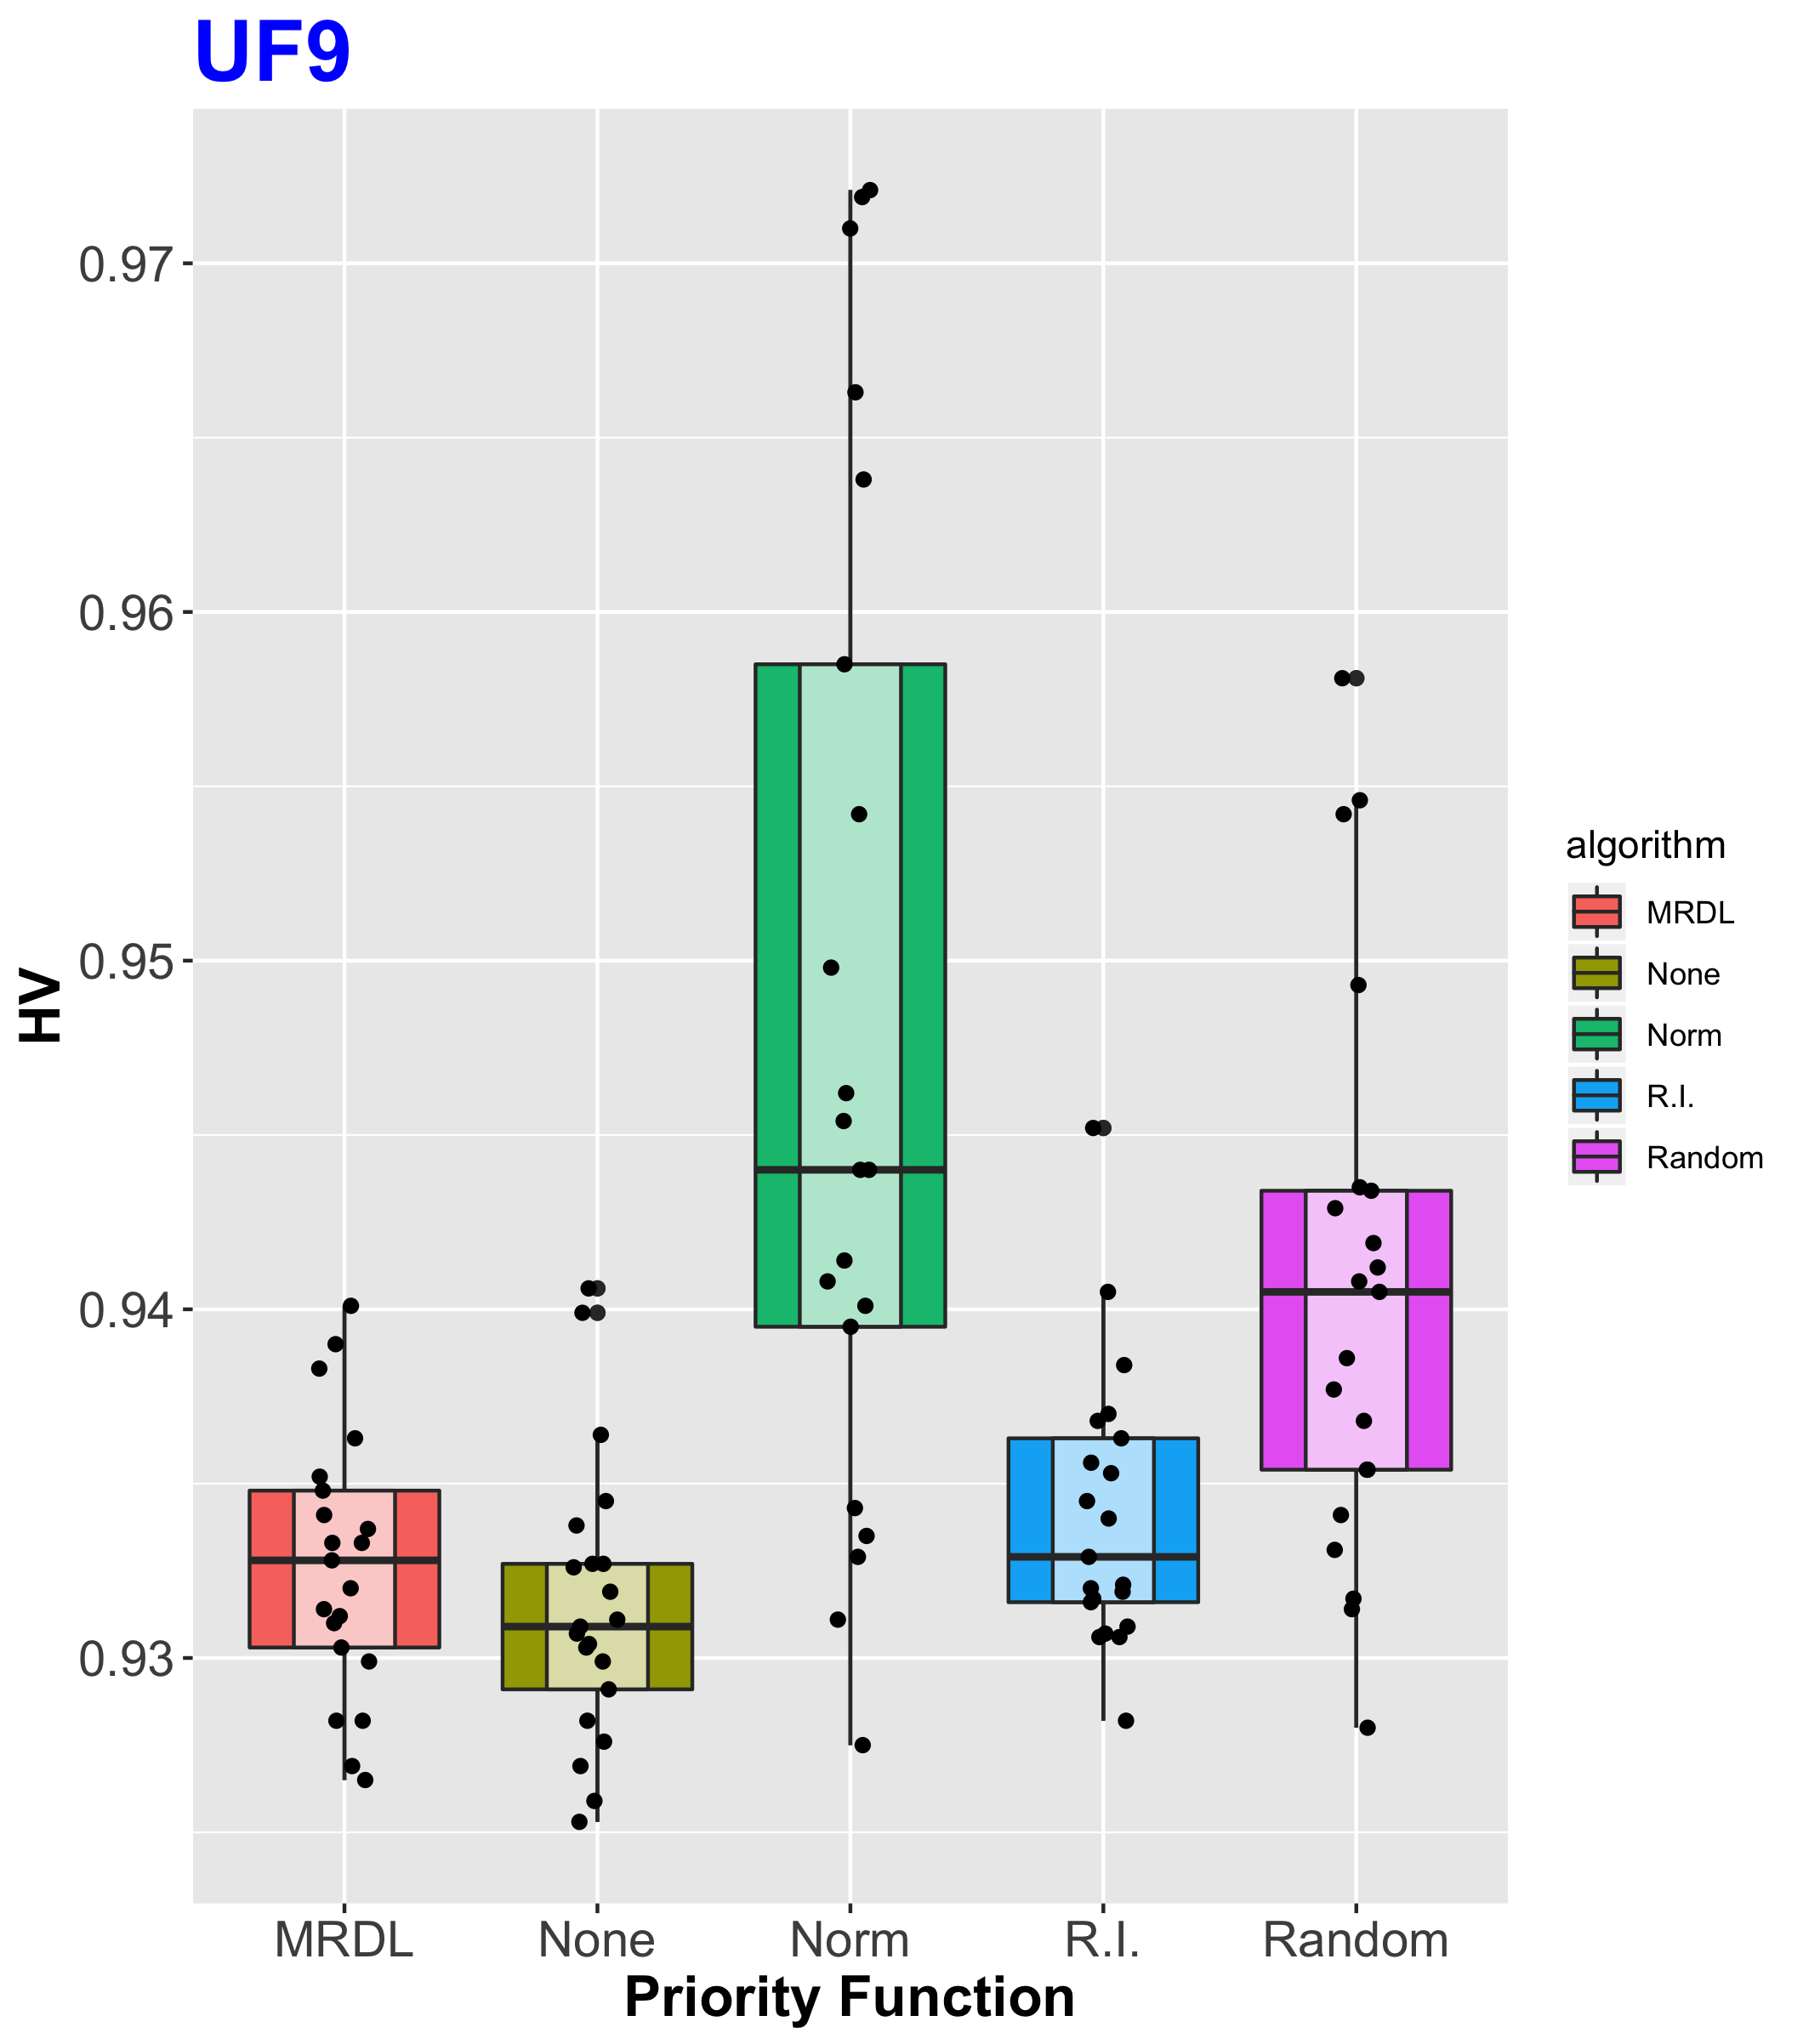
\includegraphics[width=1\textwidth, height=0.8\textwidth]{images/UF9_HV.png}
%	\caption{HV - UF3}
	\end{subfigure}
	\begin{subfigure}[b]{0.33\textwidth}
		\centering
	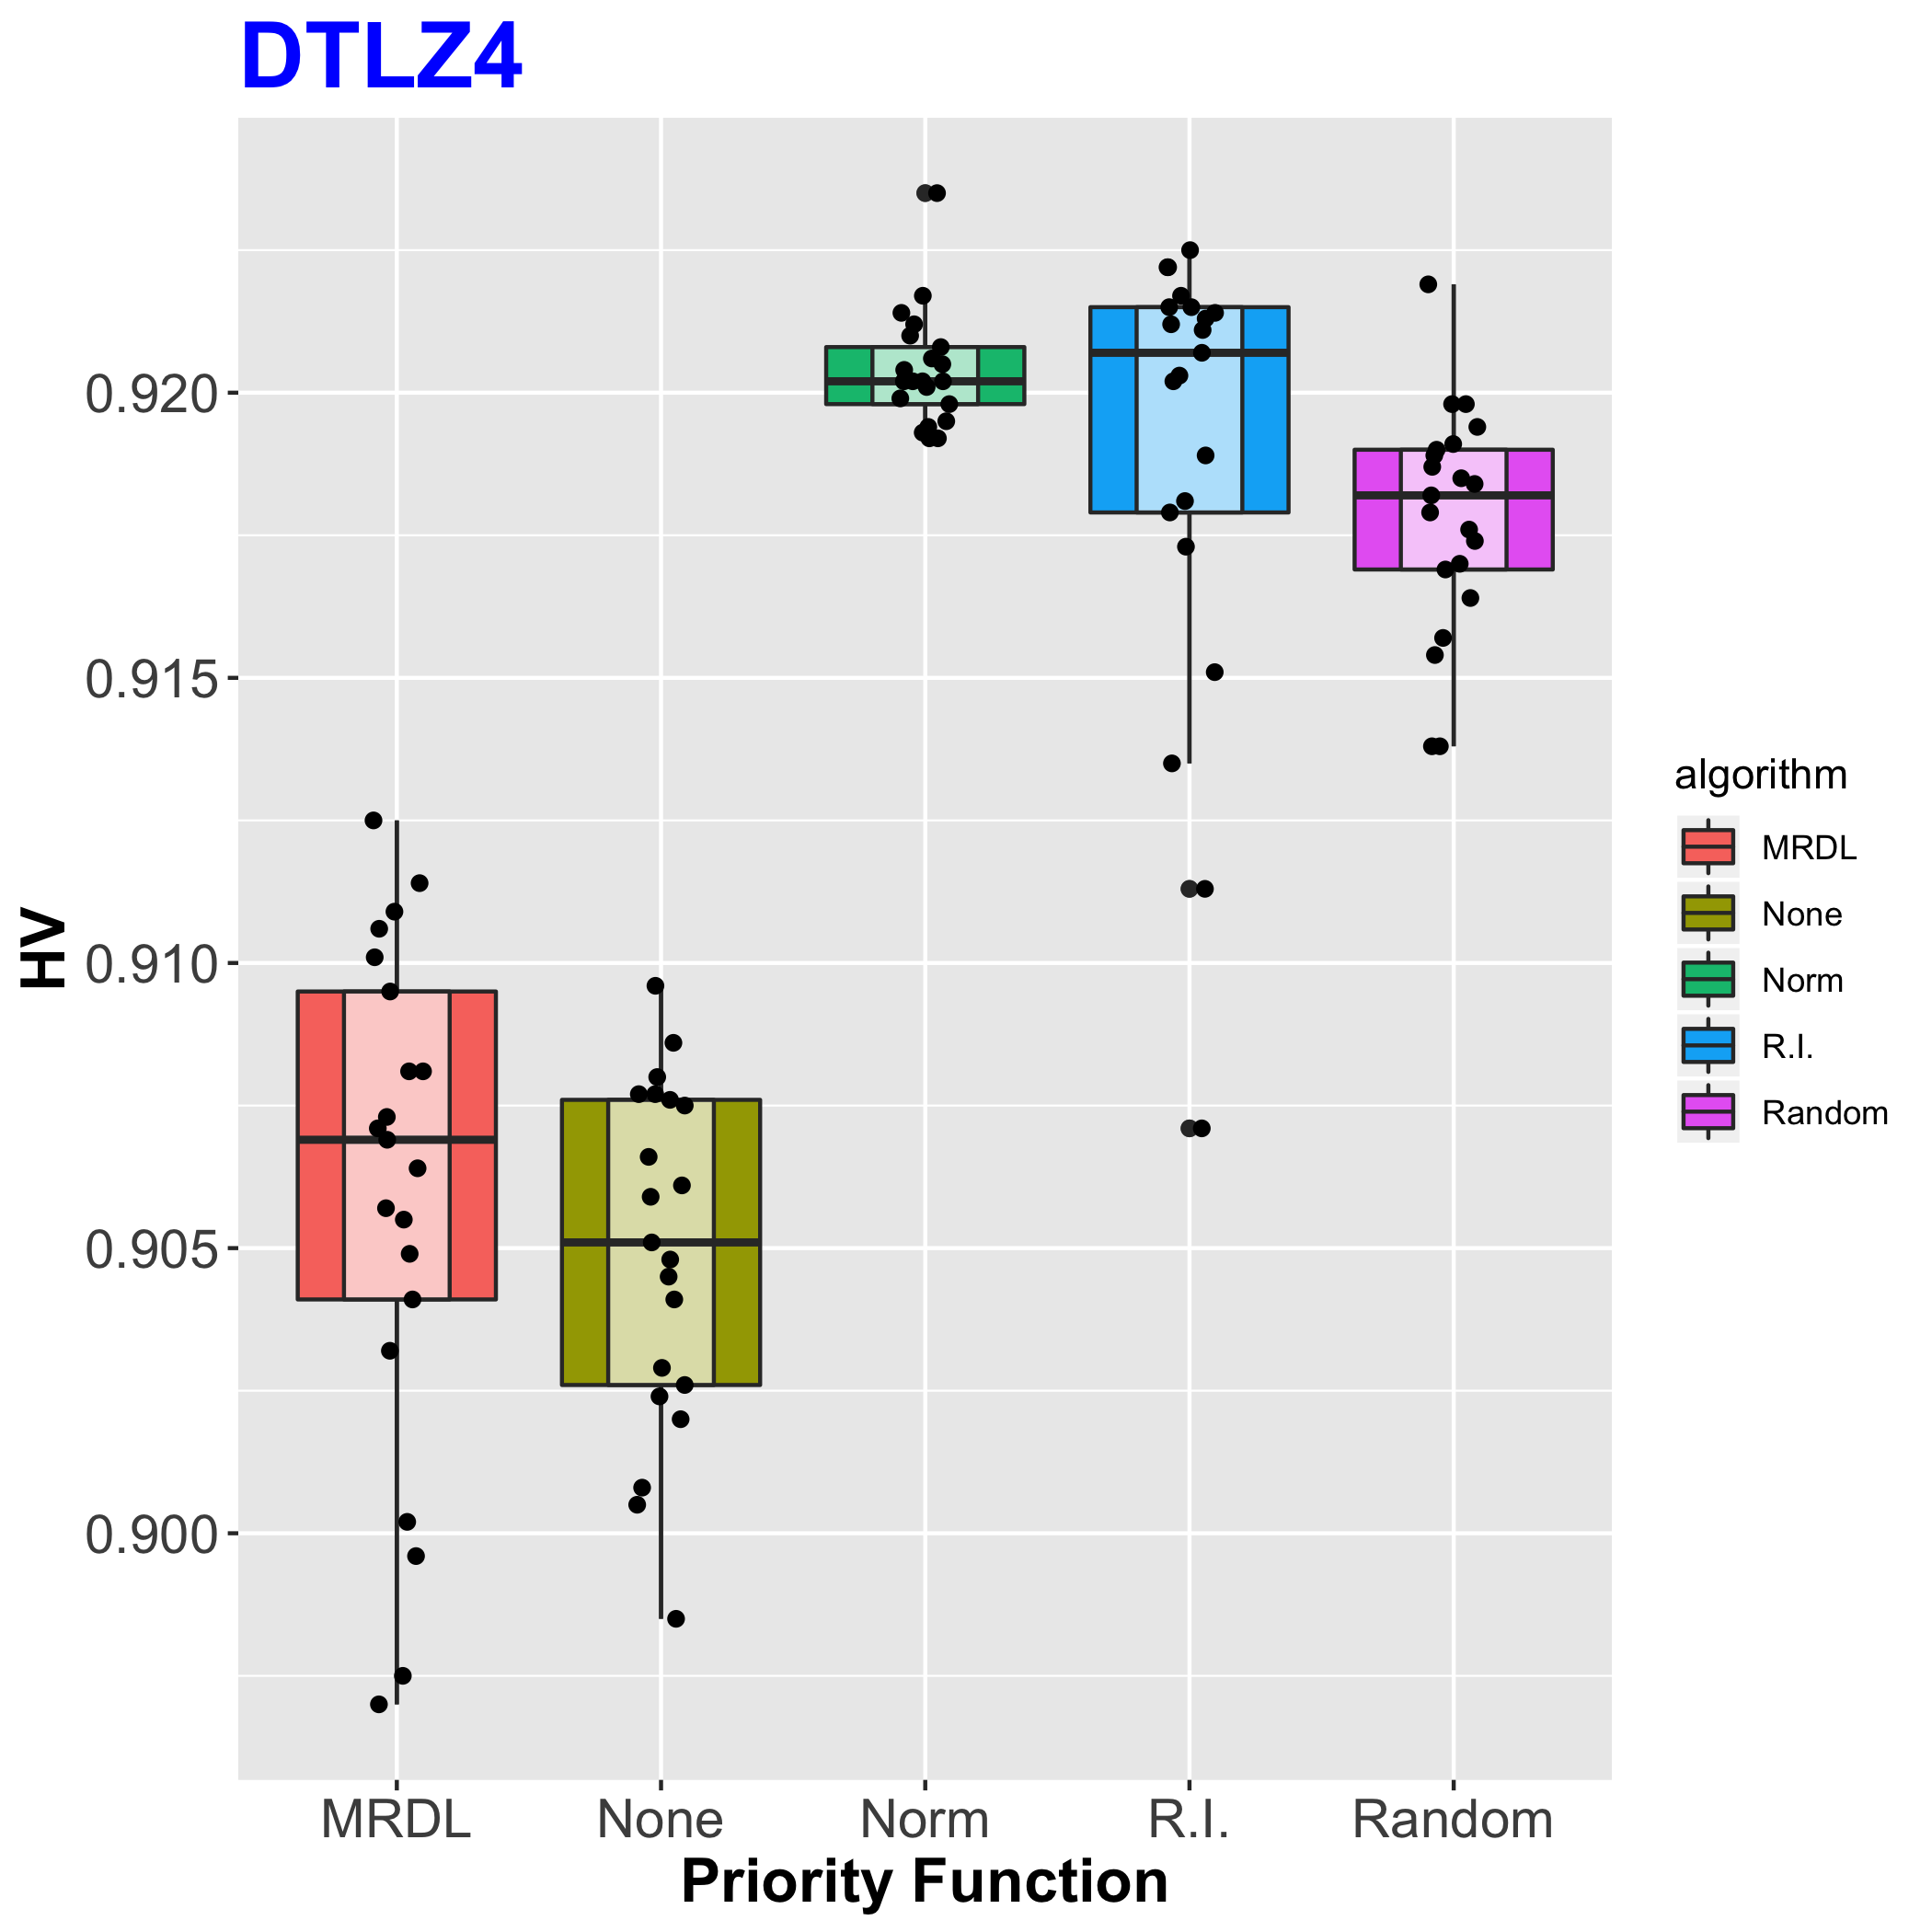
\includegraphics[width=1\textwidth, height=0.8\textwidth]{images/DTLZ4_HV.png}
%	\caption{HV - UF8}
	\end{subfigure}
\begin{subfigure}[b]{0.33\textwidth}
	\centering
	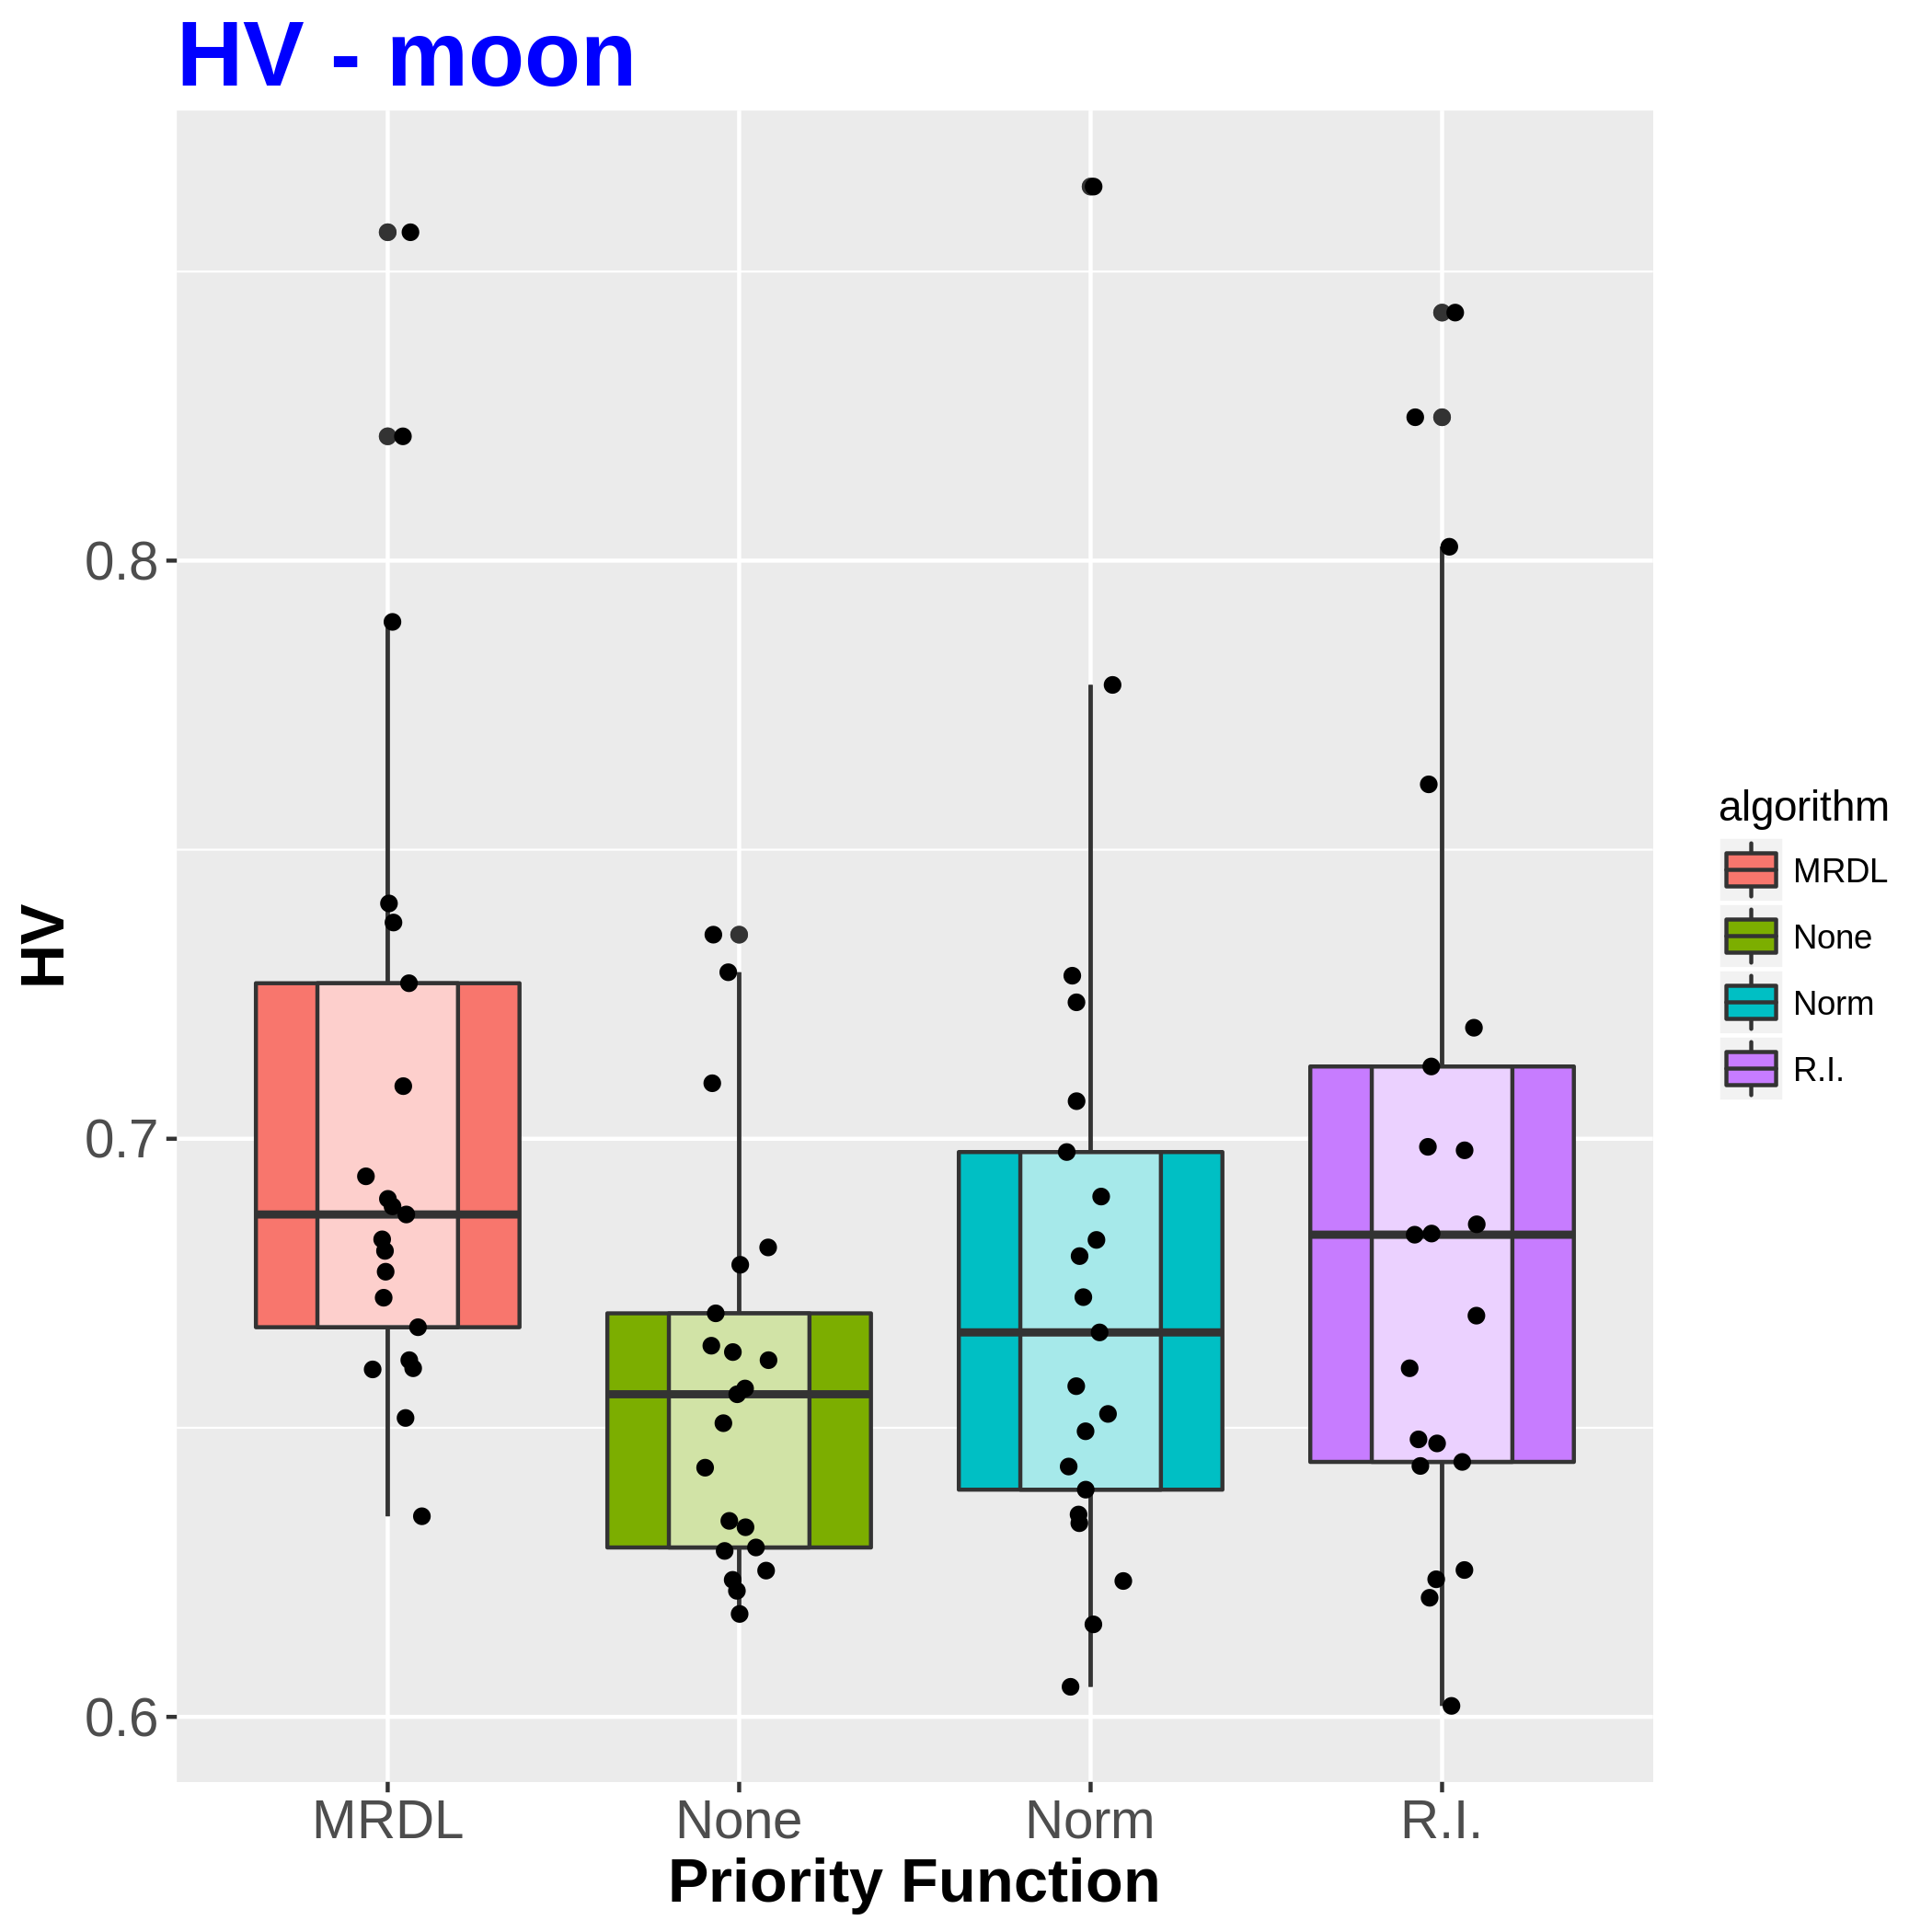
\includegraphics[width=1\textwidth, height=0.8\textwidth]{images/moon_HV.png}
%	\caption{HV - DTLZ4}
\end{subfigure}
	\caption{Box plot of HV values on UF9, DTLZ4 and Lunar Landing.None is the MOEA/D-DE with no priority function.}
		\label{HVS}
\end{figure*}

%\begin{figure*}[!t]
%%	\Large{Average performance on different tournament size - Gallagher's Gaussian 21-hi Peaks Function}
%	\begin{subfigure}[b]{0.33\textwidth}
%		\centering
%		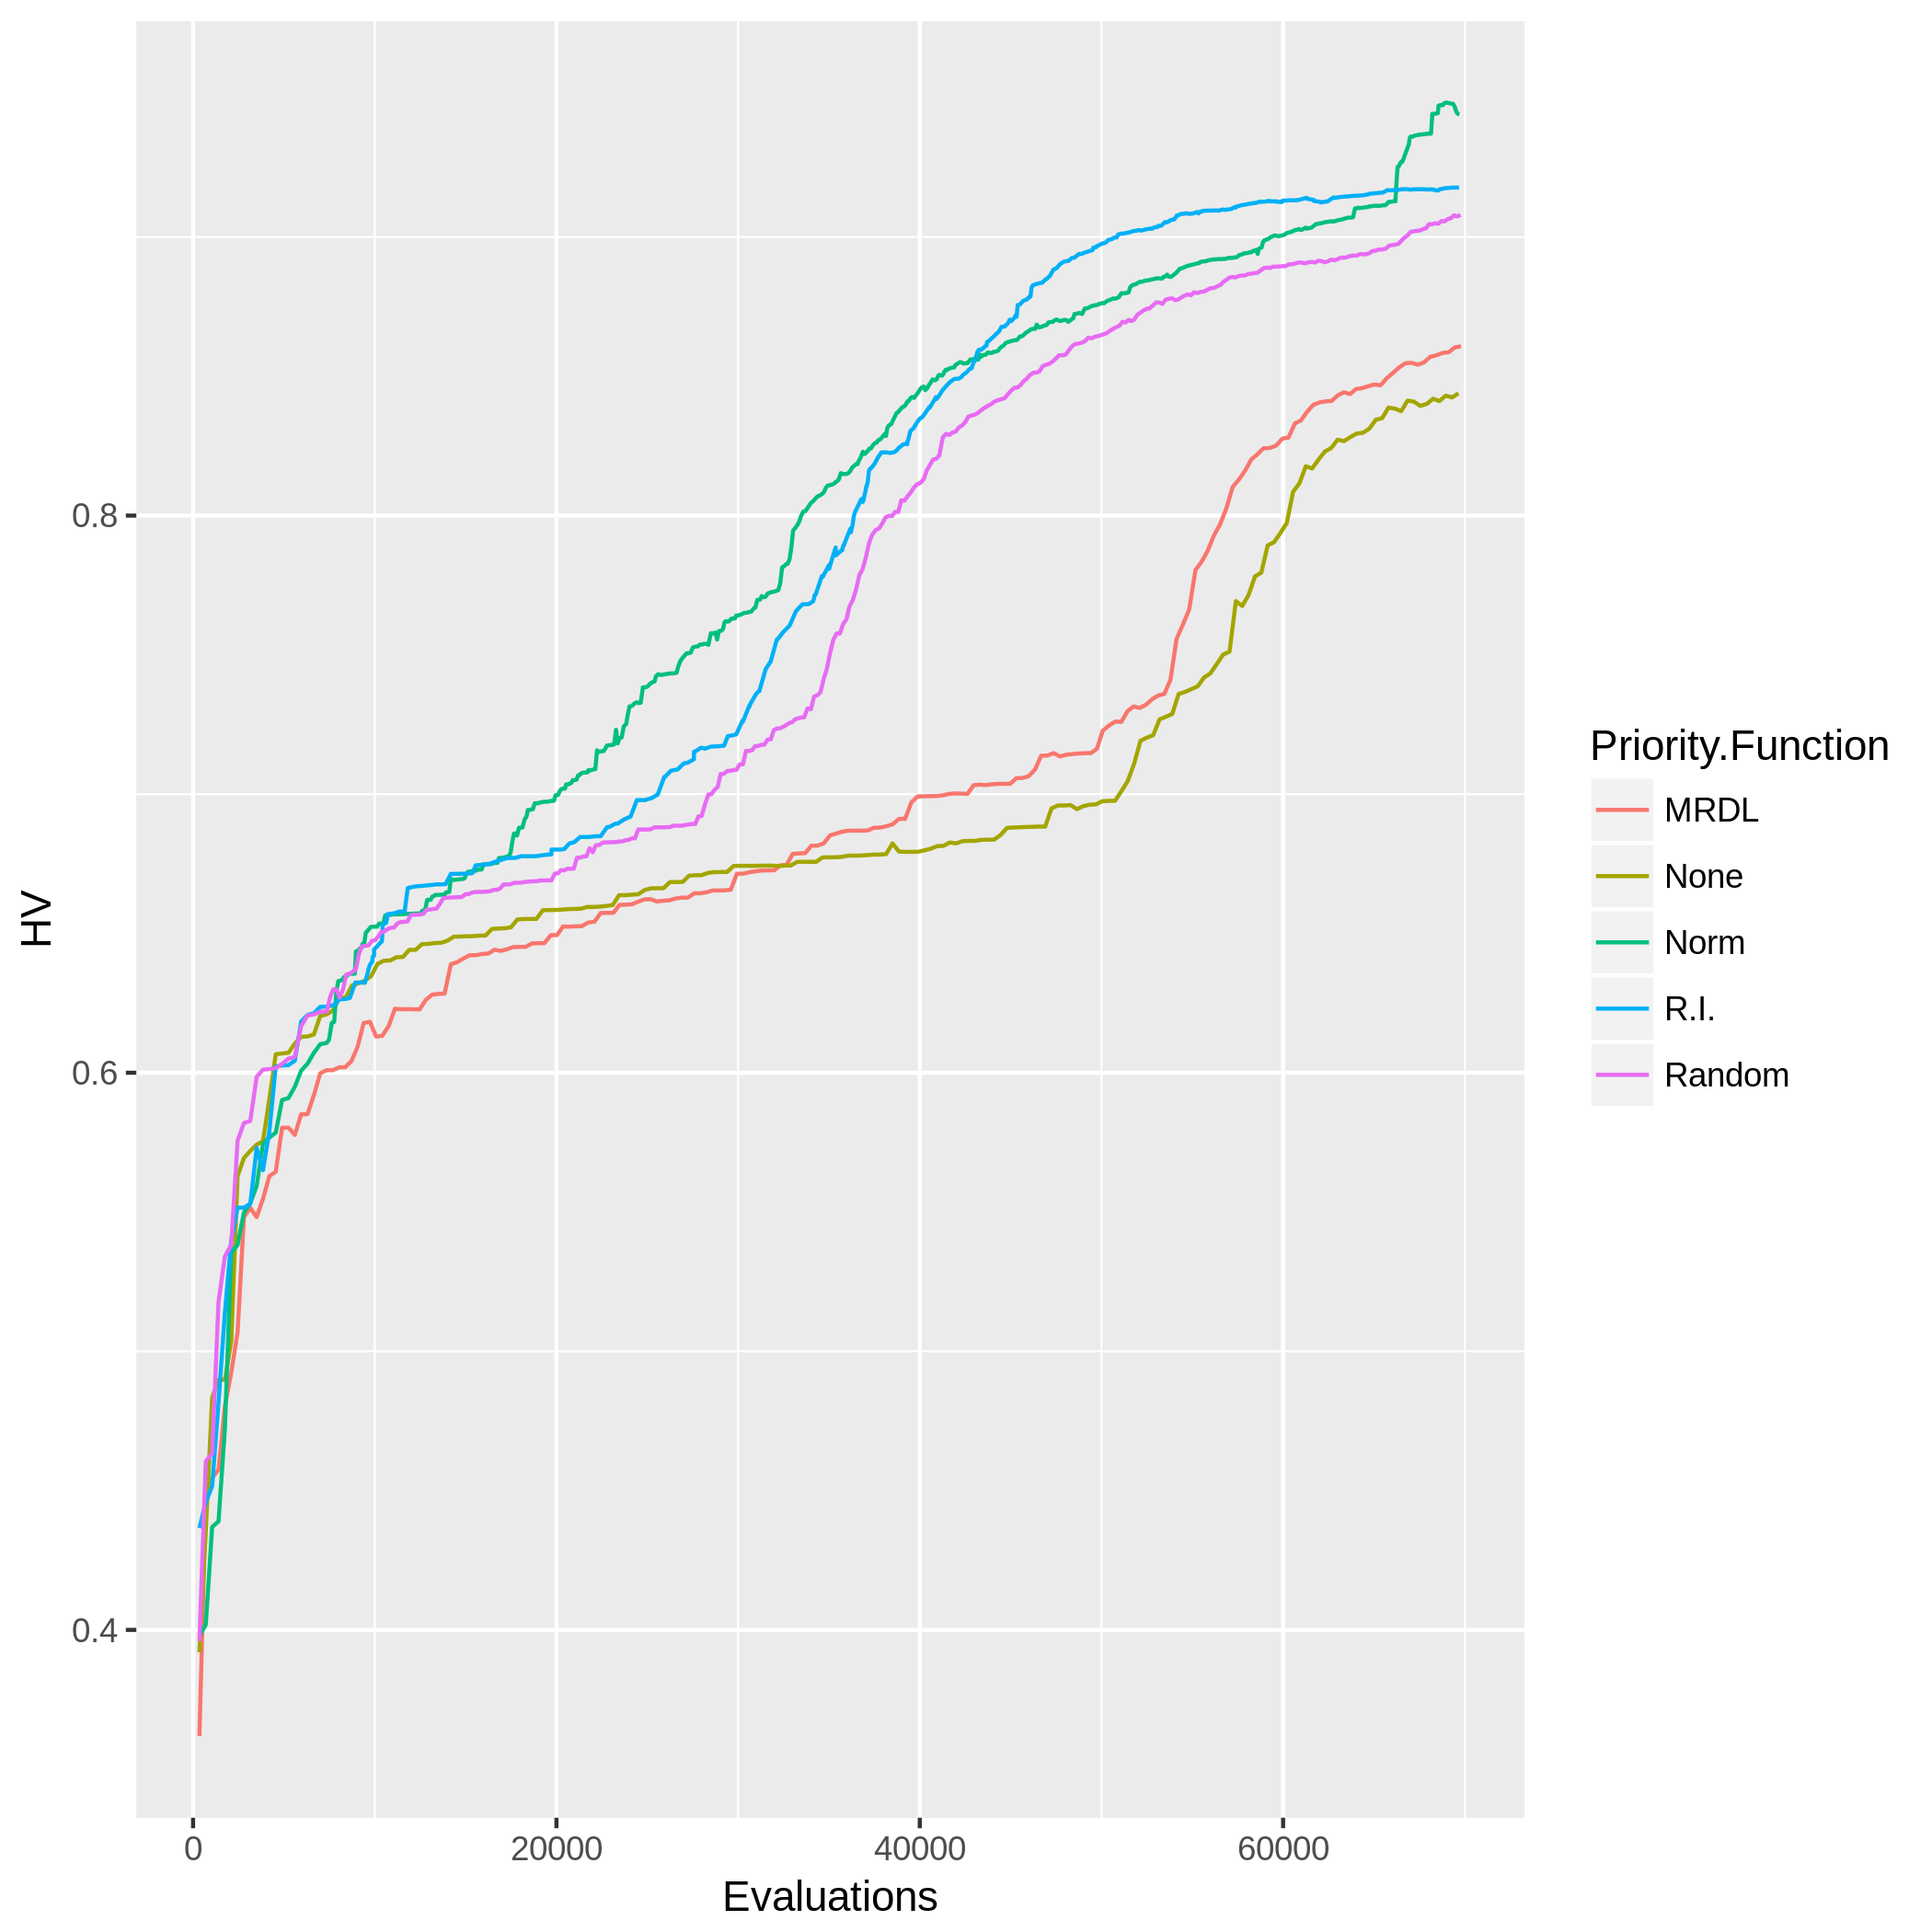
\includegraphics[width=1\textwidth, height=1\textwidth]{images/UF3hv_all}
%	\caption{Evolution - UF3}
%	\end{subfigure}
%	\begin{subfigure}[b]{0.33\textwidth}
%		\centering
%		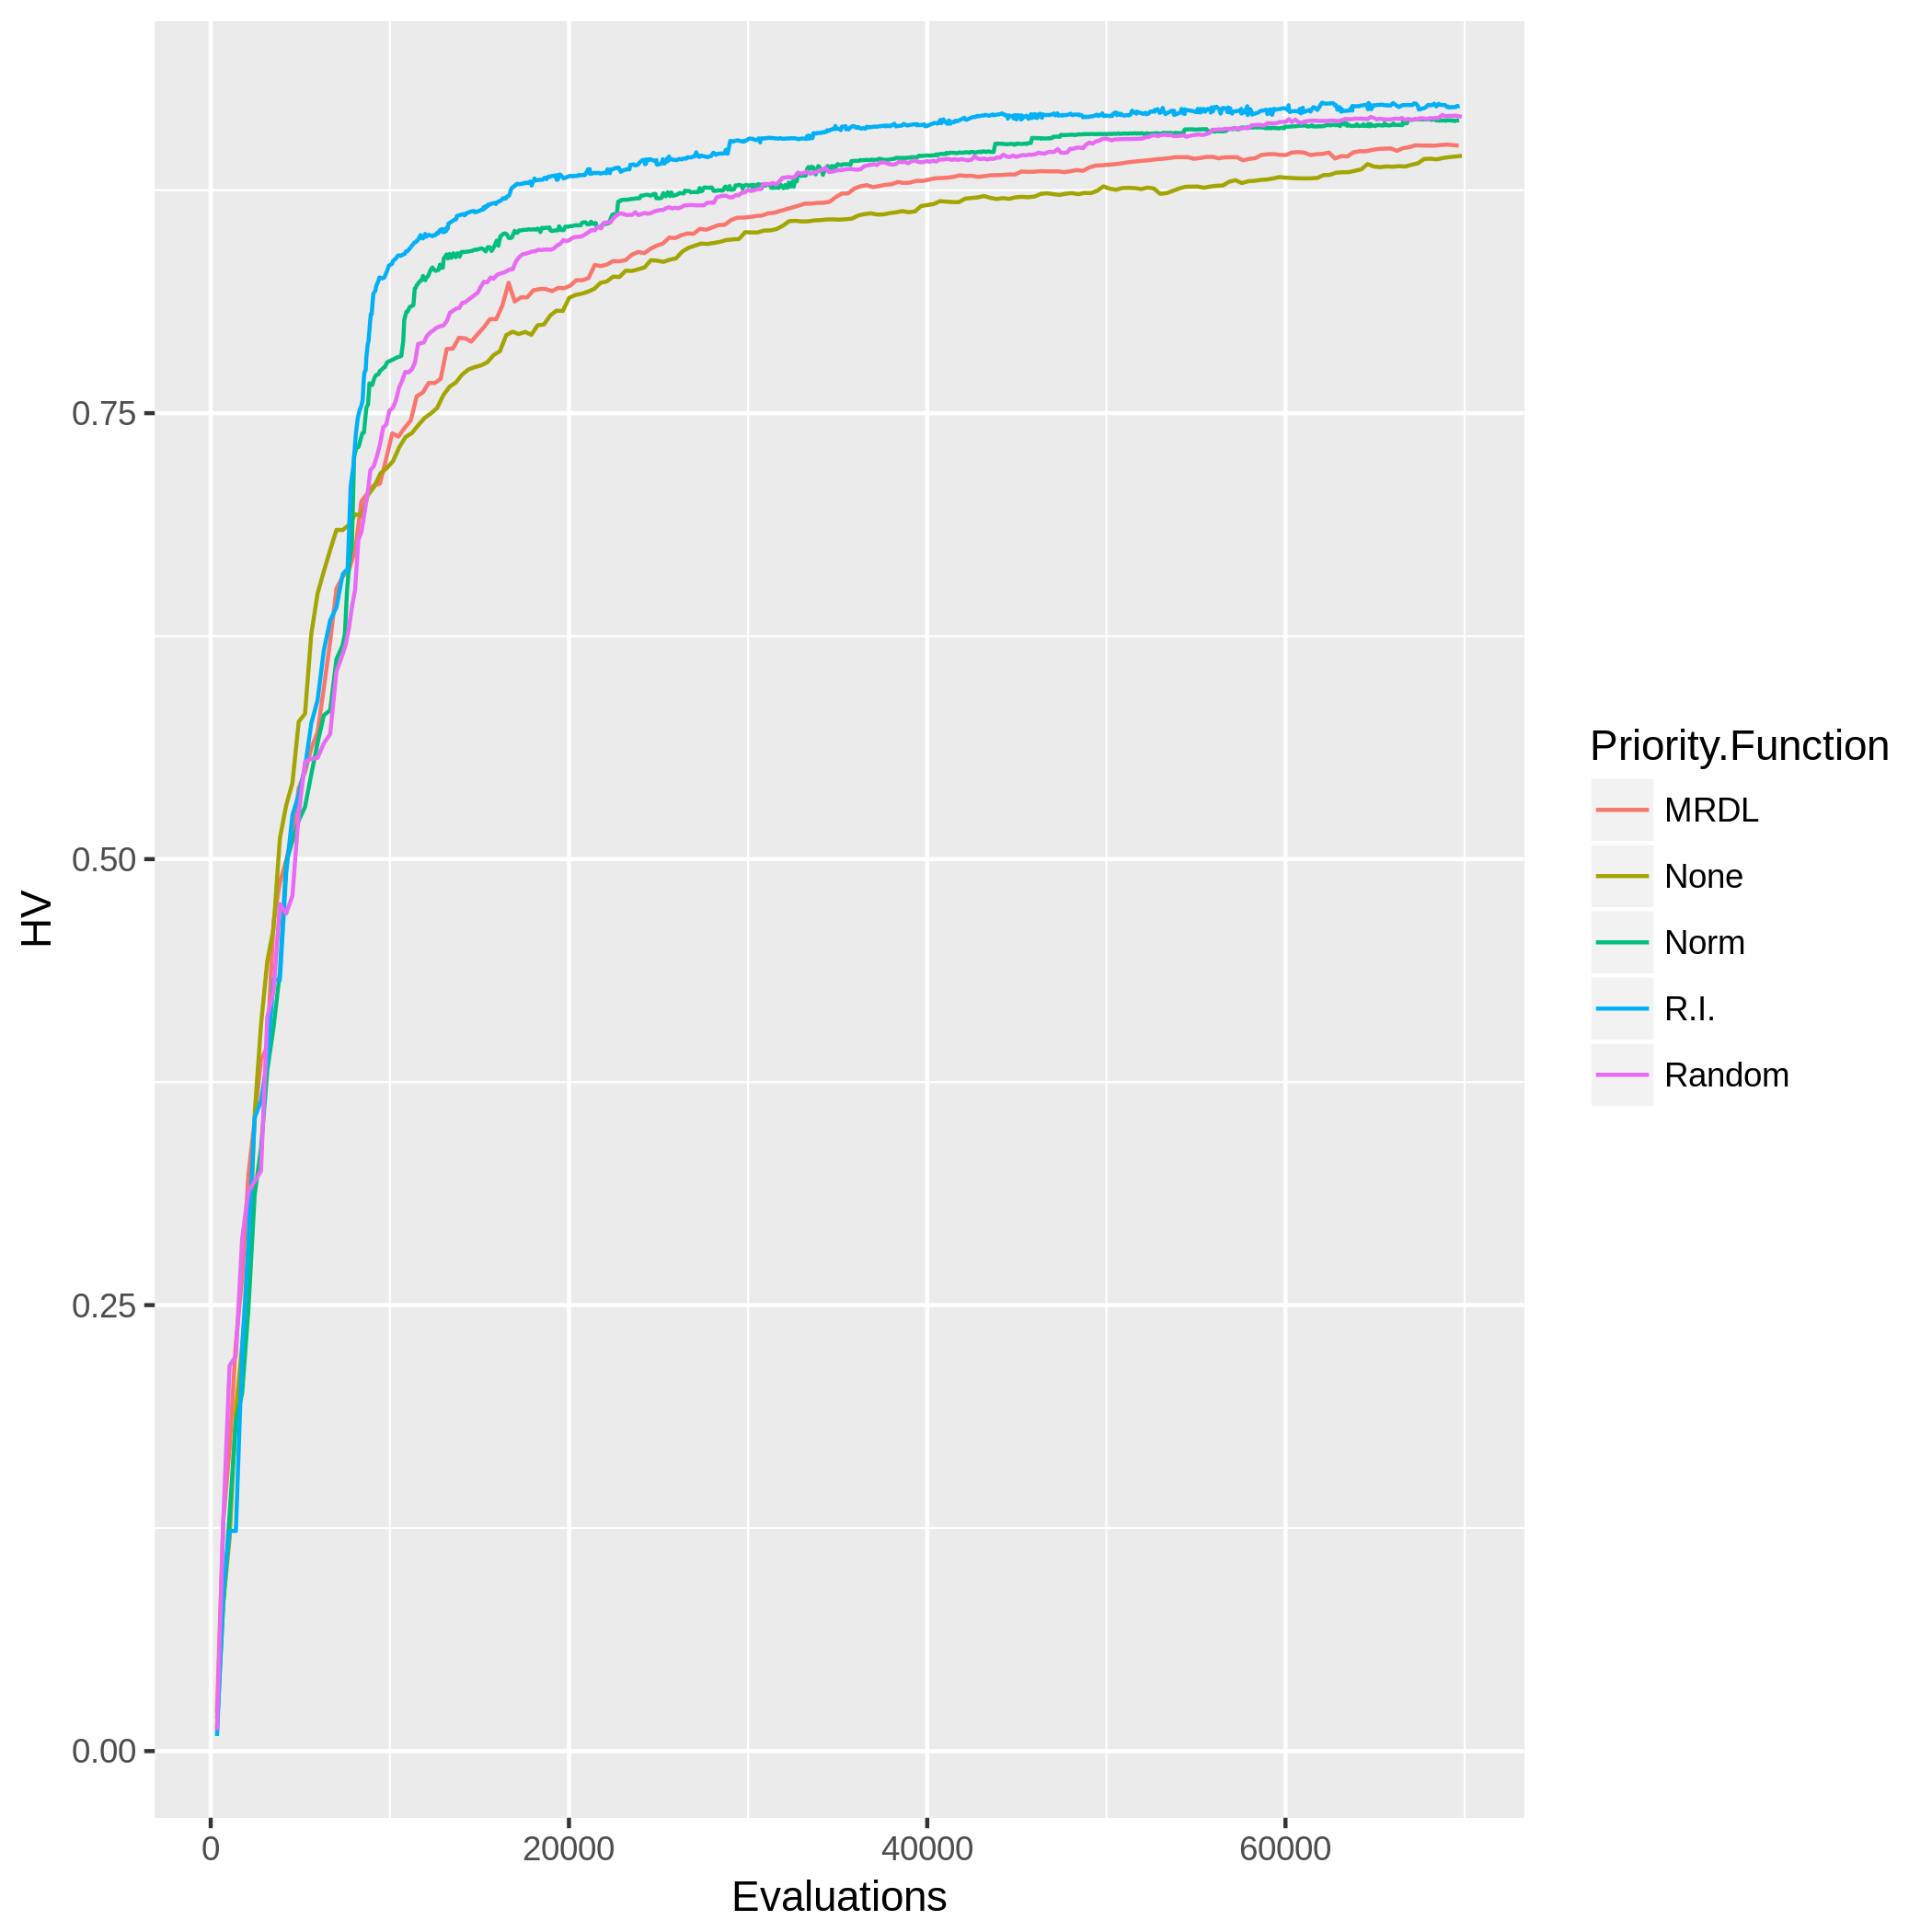
\includegraphics[width=1\textwidth, height=1\textwidth]{images/UF8hv_all}
%	\caption{Evolution - UF8}
%	\end{subfigure}
%\begin{subfigure}[b]{0.33\textwidth}
%	\centering
%	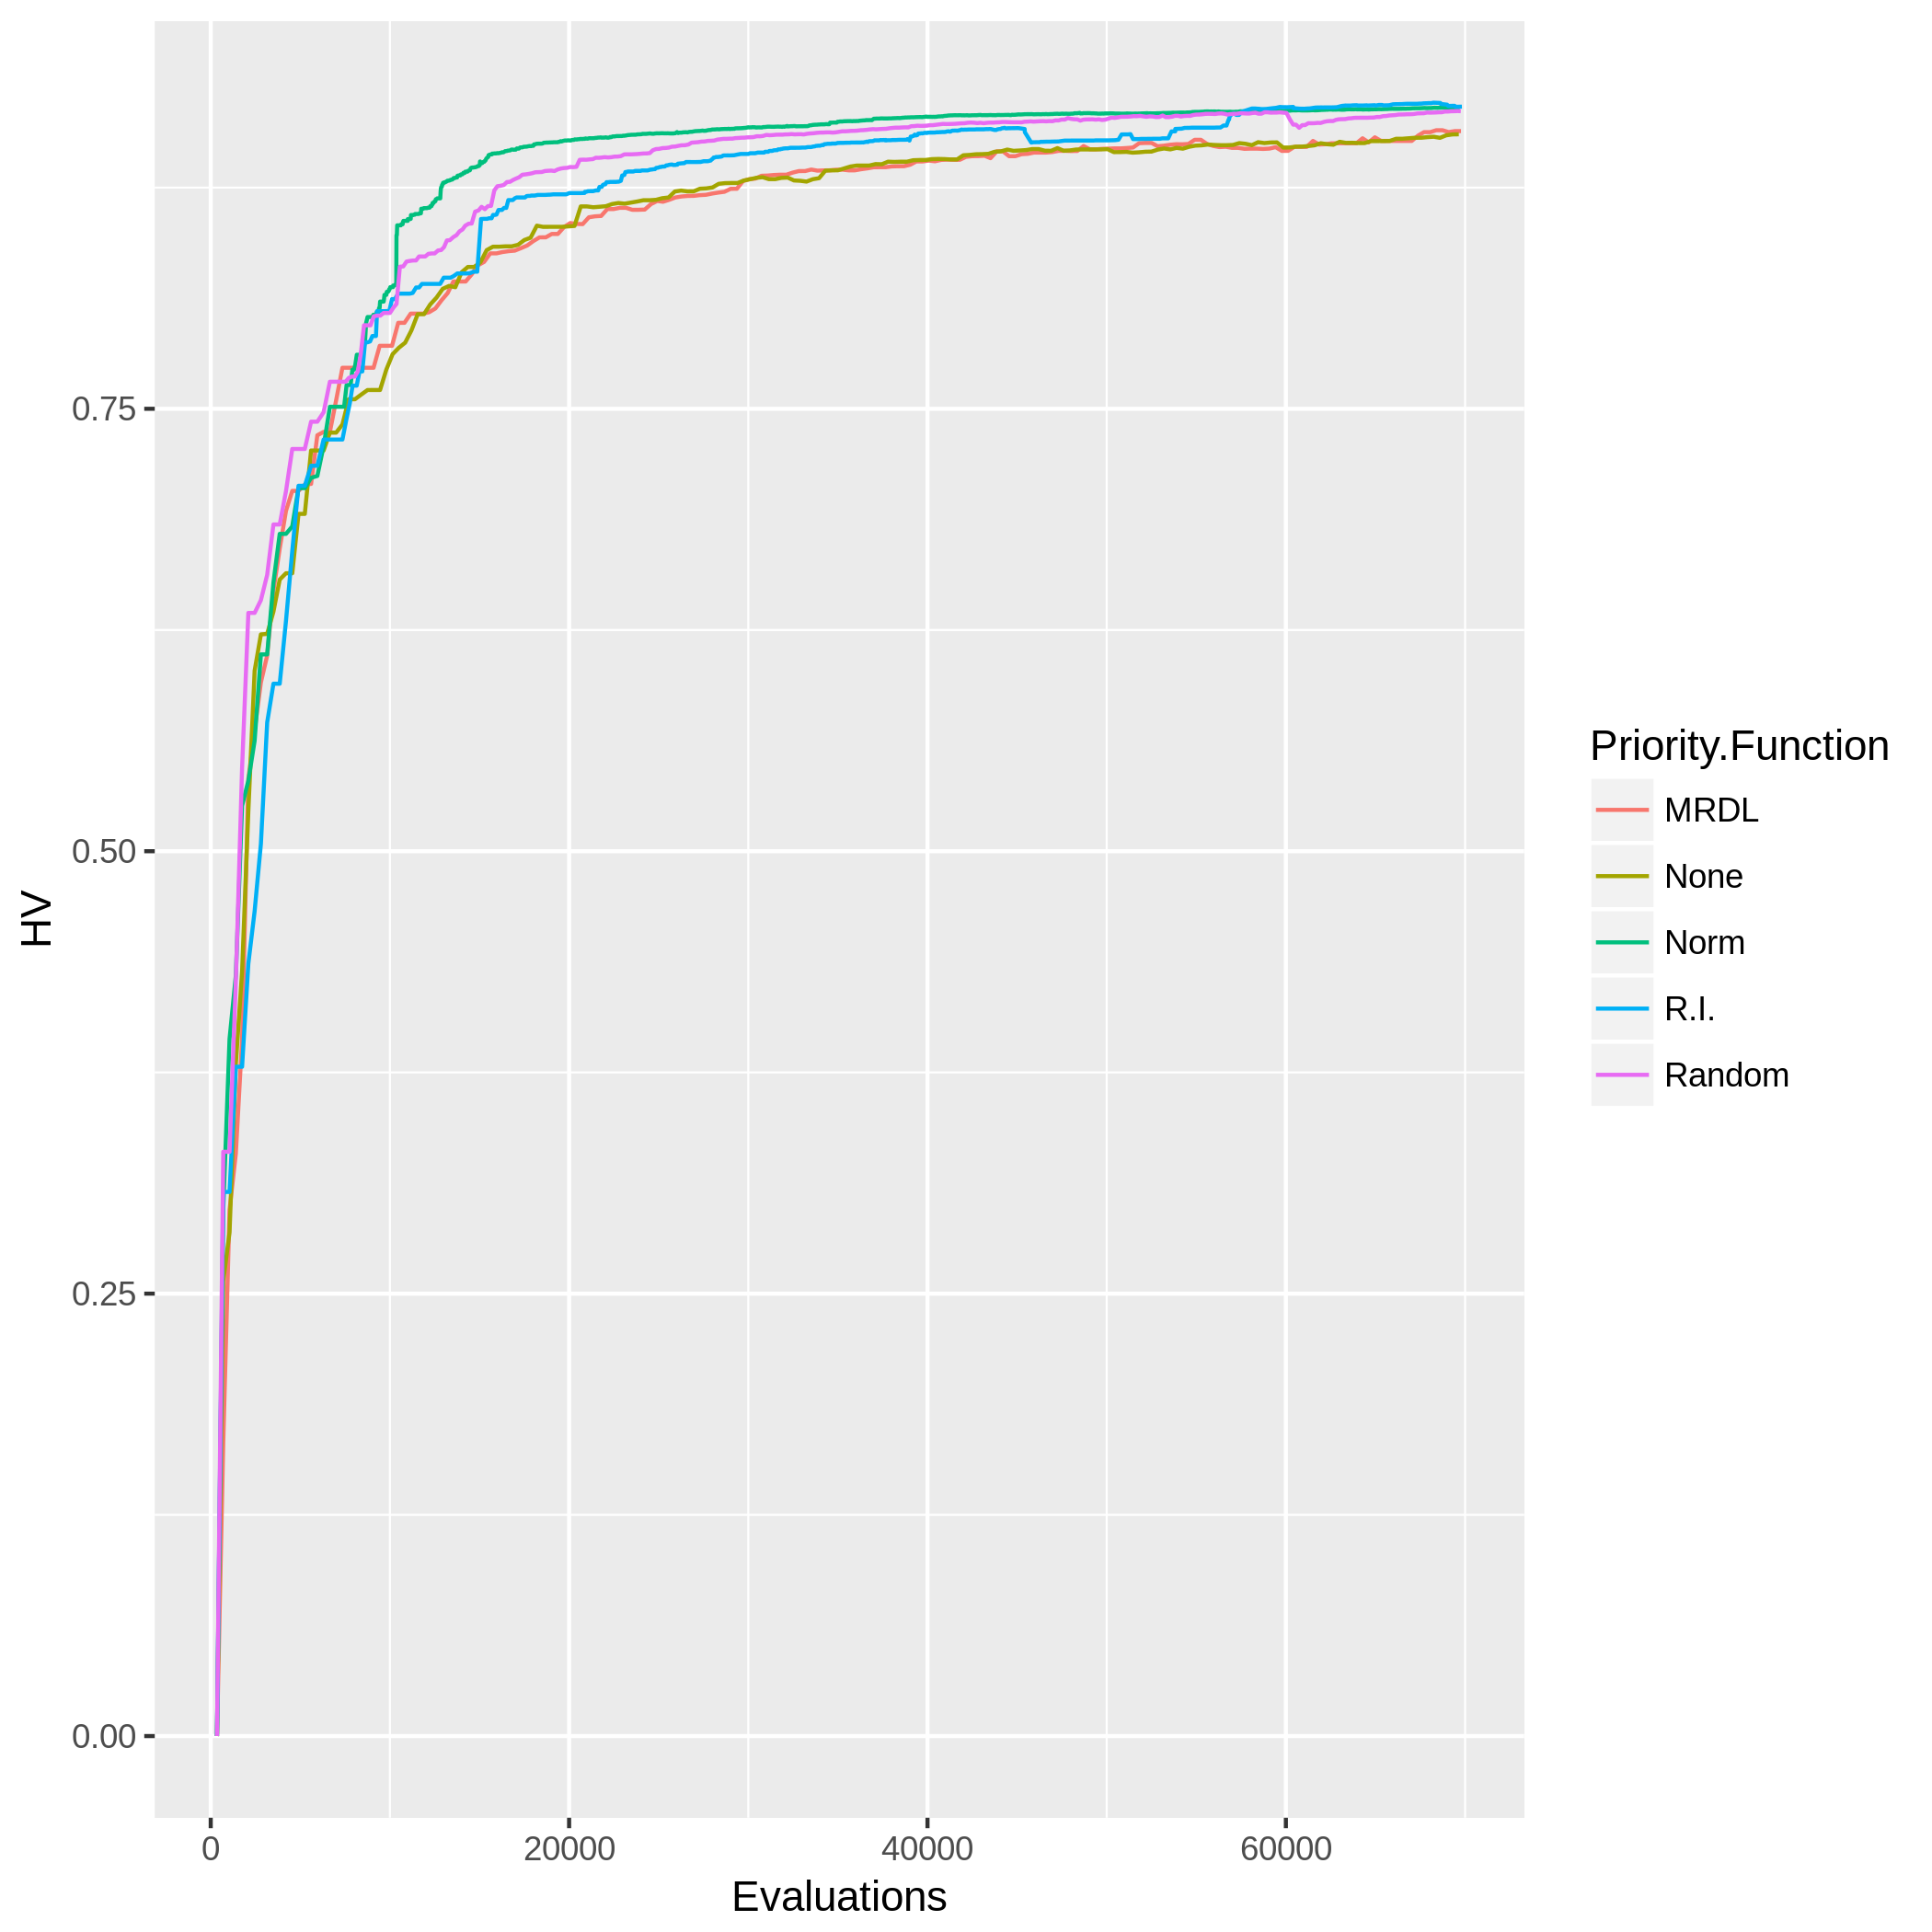
\includegraphics[width=1\textwidth, height=1\textwidth]{images/DTLZ4hv_all}
%	\caption{Evolution - DTLZ4}
%\end{subfigure}
%	\caption{Evolution of HV values on Artificial Benchmark Problems}
%\label{evolution_hv}
%\end{figure*}

\begin{figure*}[!t]

	\begin{subfigure}[b]{0.33\textwidth}
		\centering
		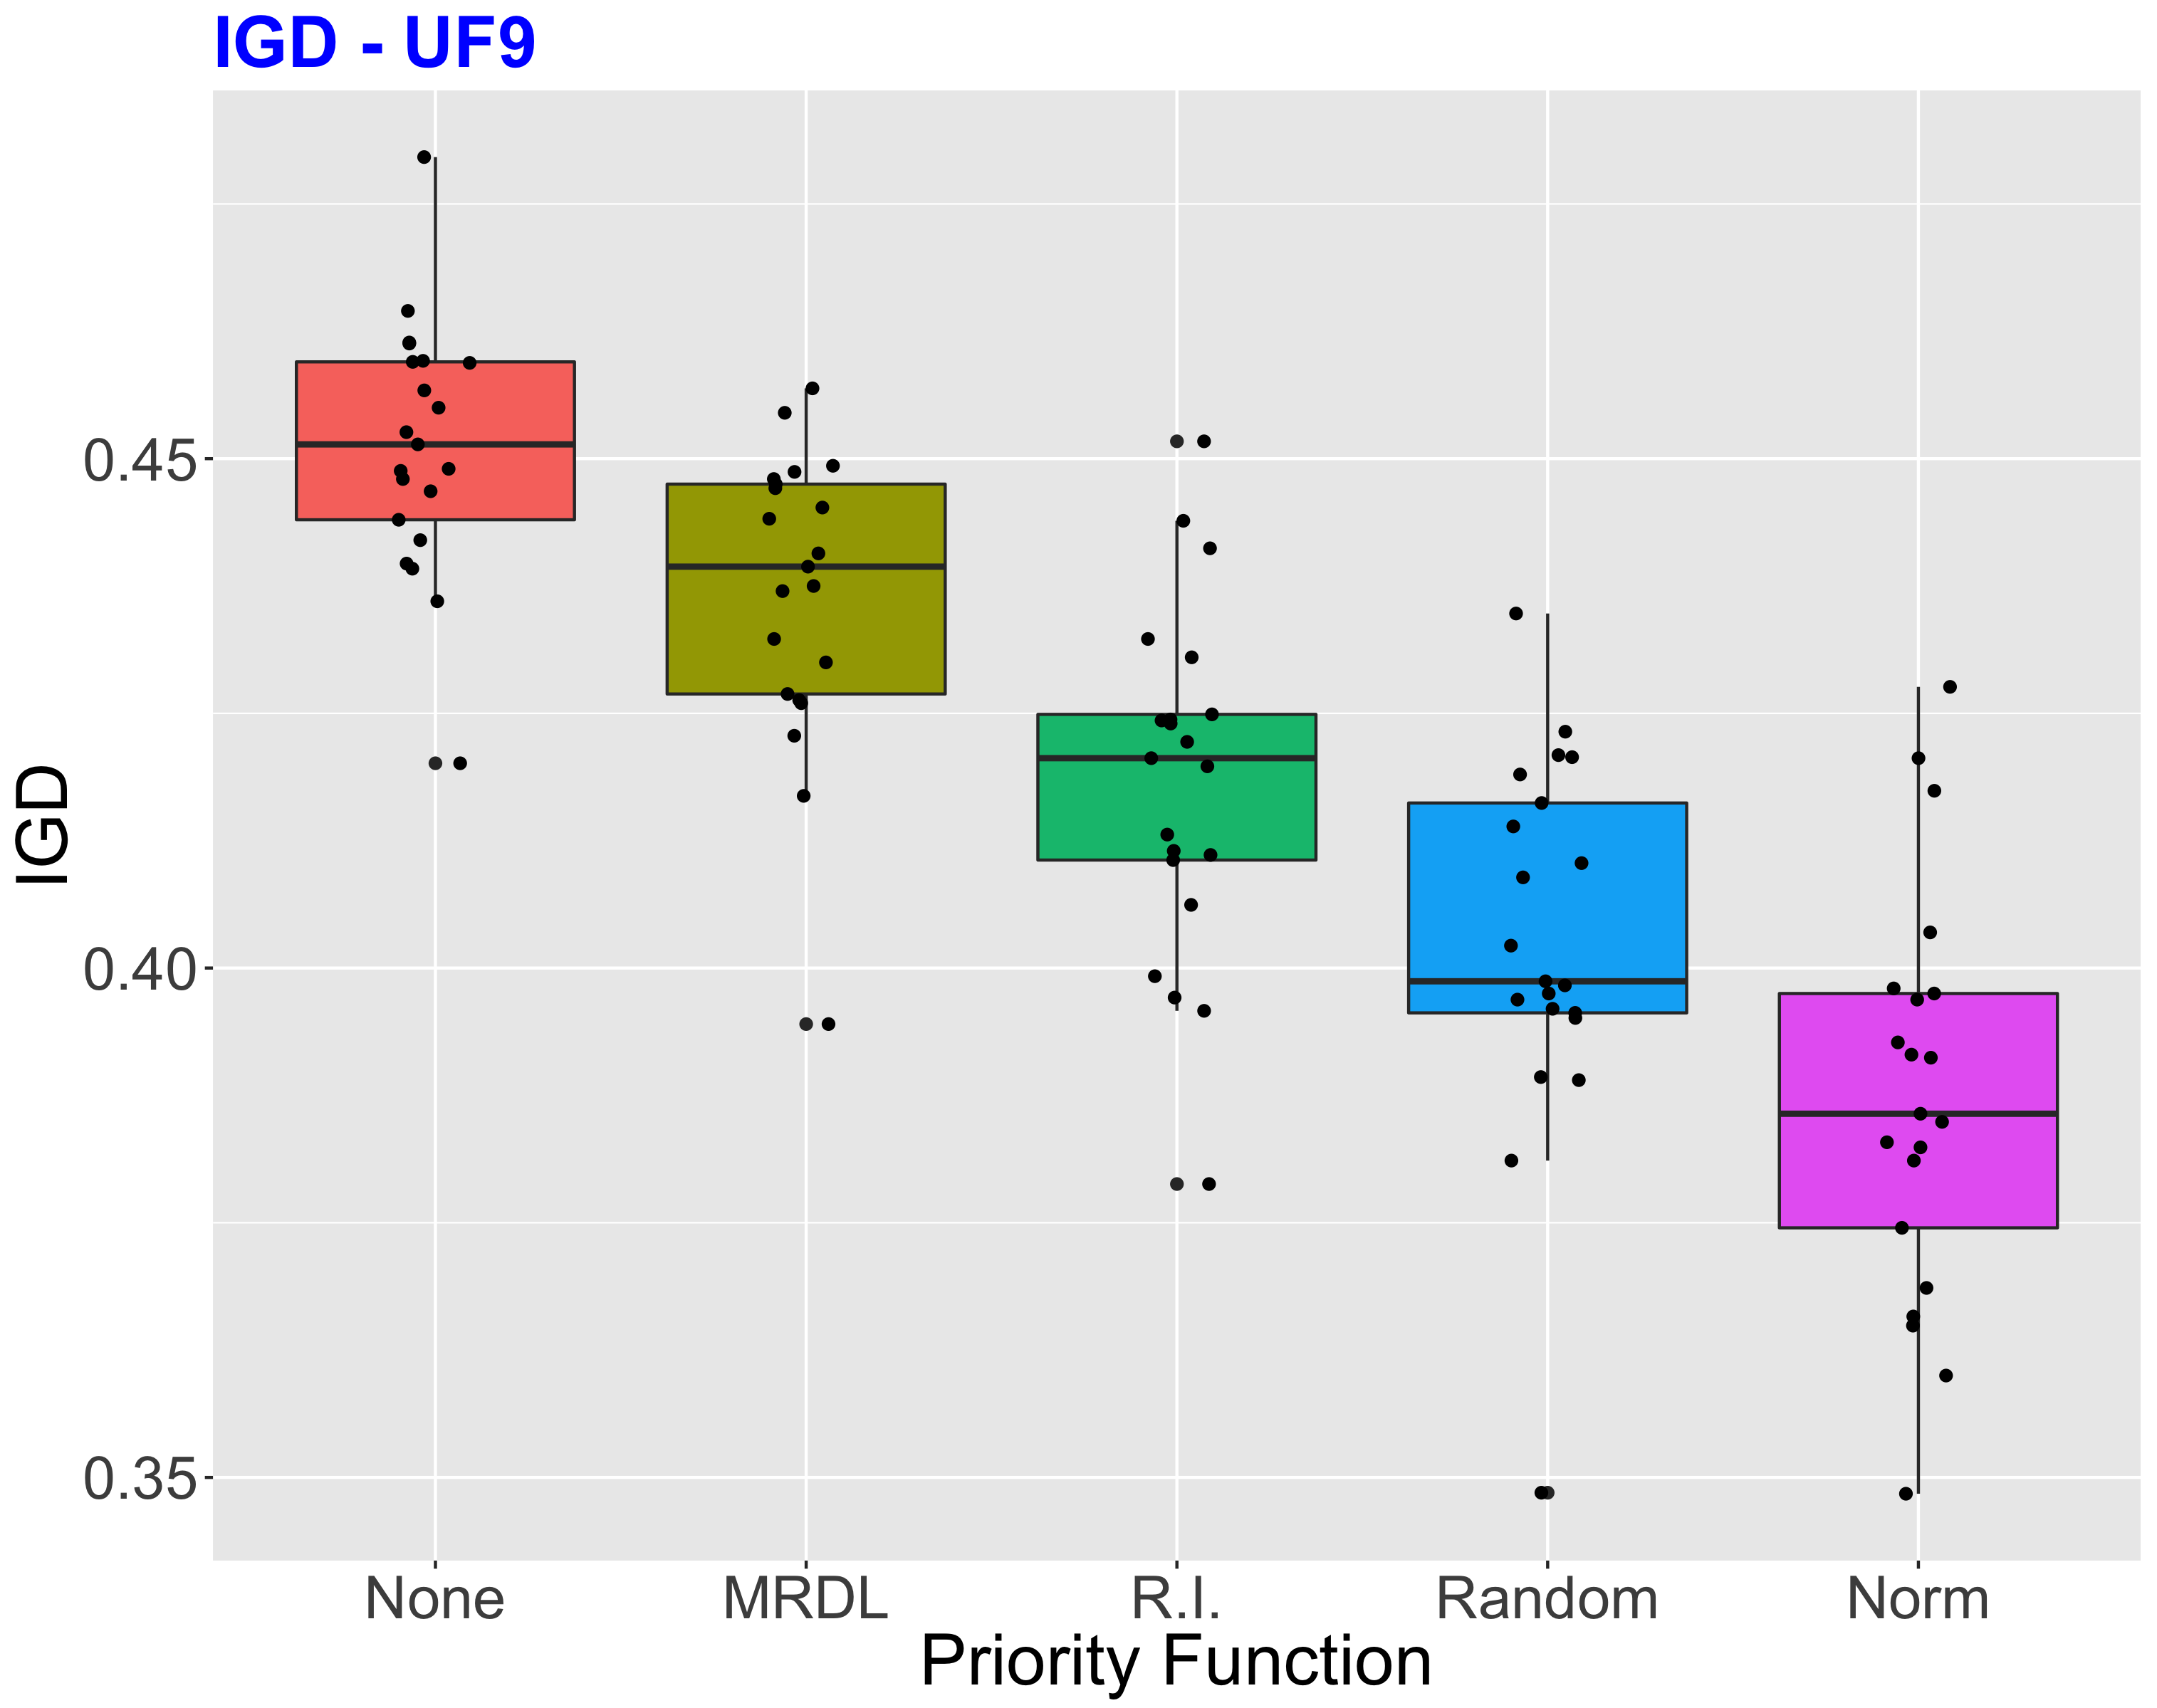
\includegraphics[width=1\textwidth, height=0.785\textwidth]{images/UF9_IGD.png}
%	\caption{IGD - UF3}
	\end{subfigure}
	\begin{subfigure}[b]{0.33\textwidth}
		\centering
		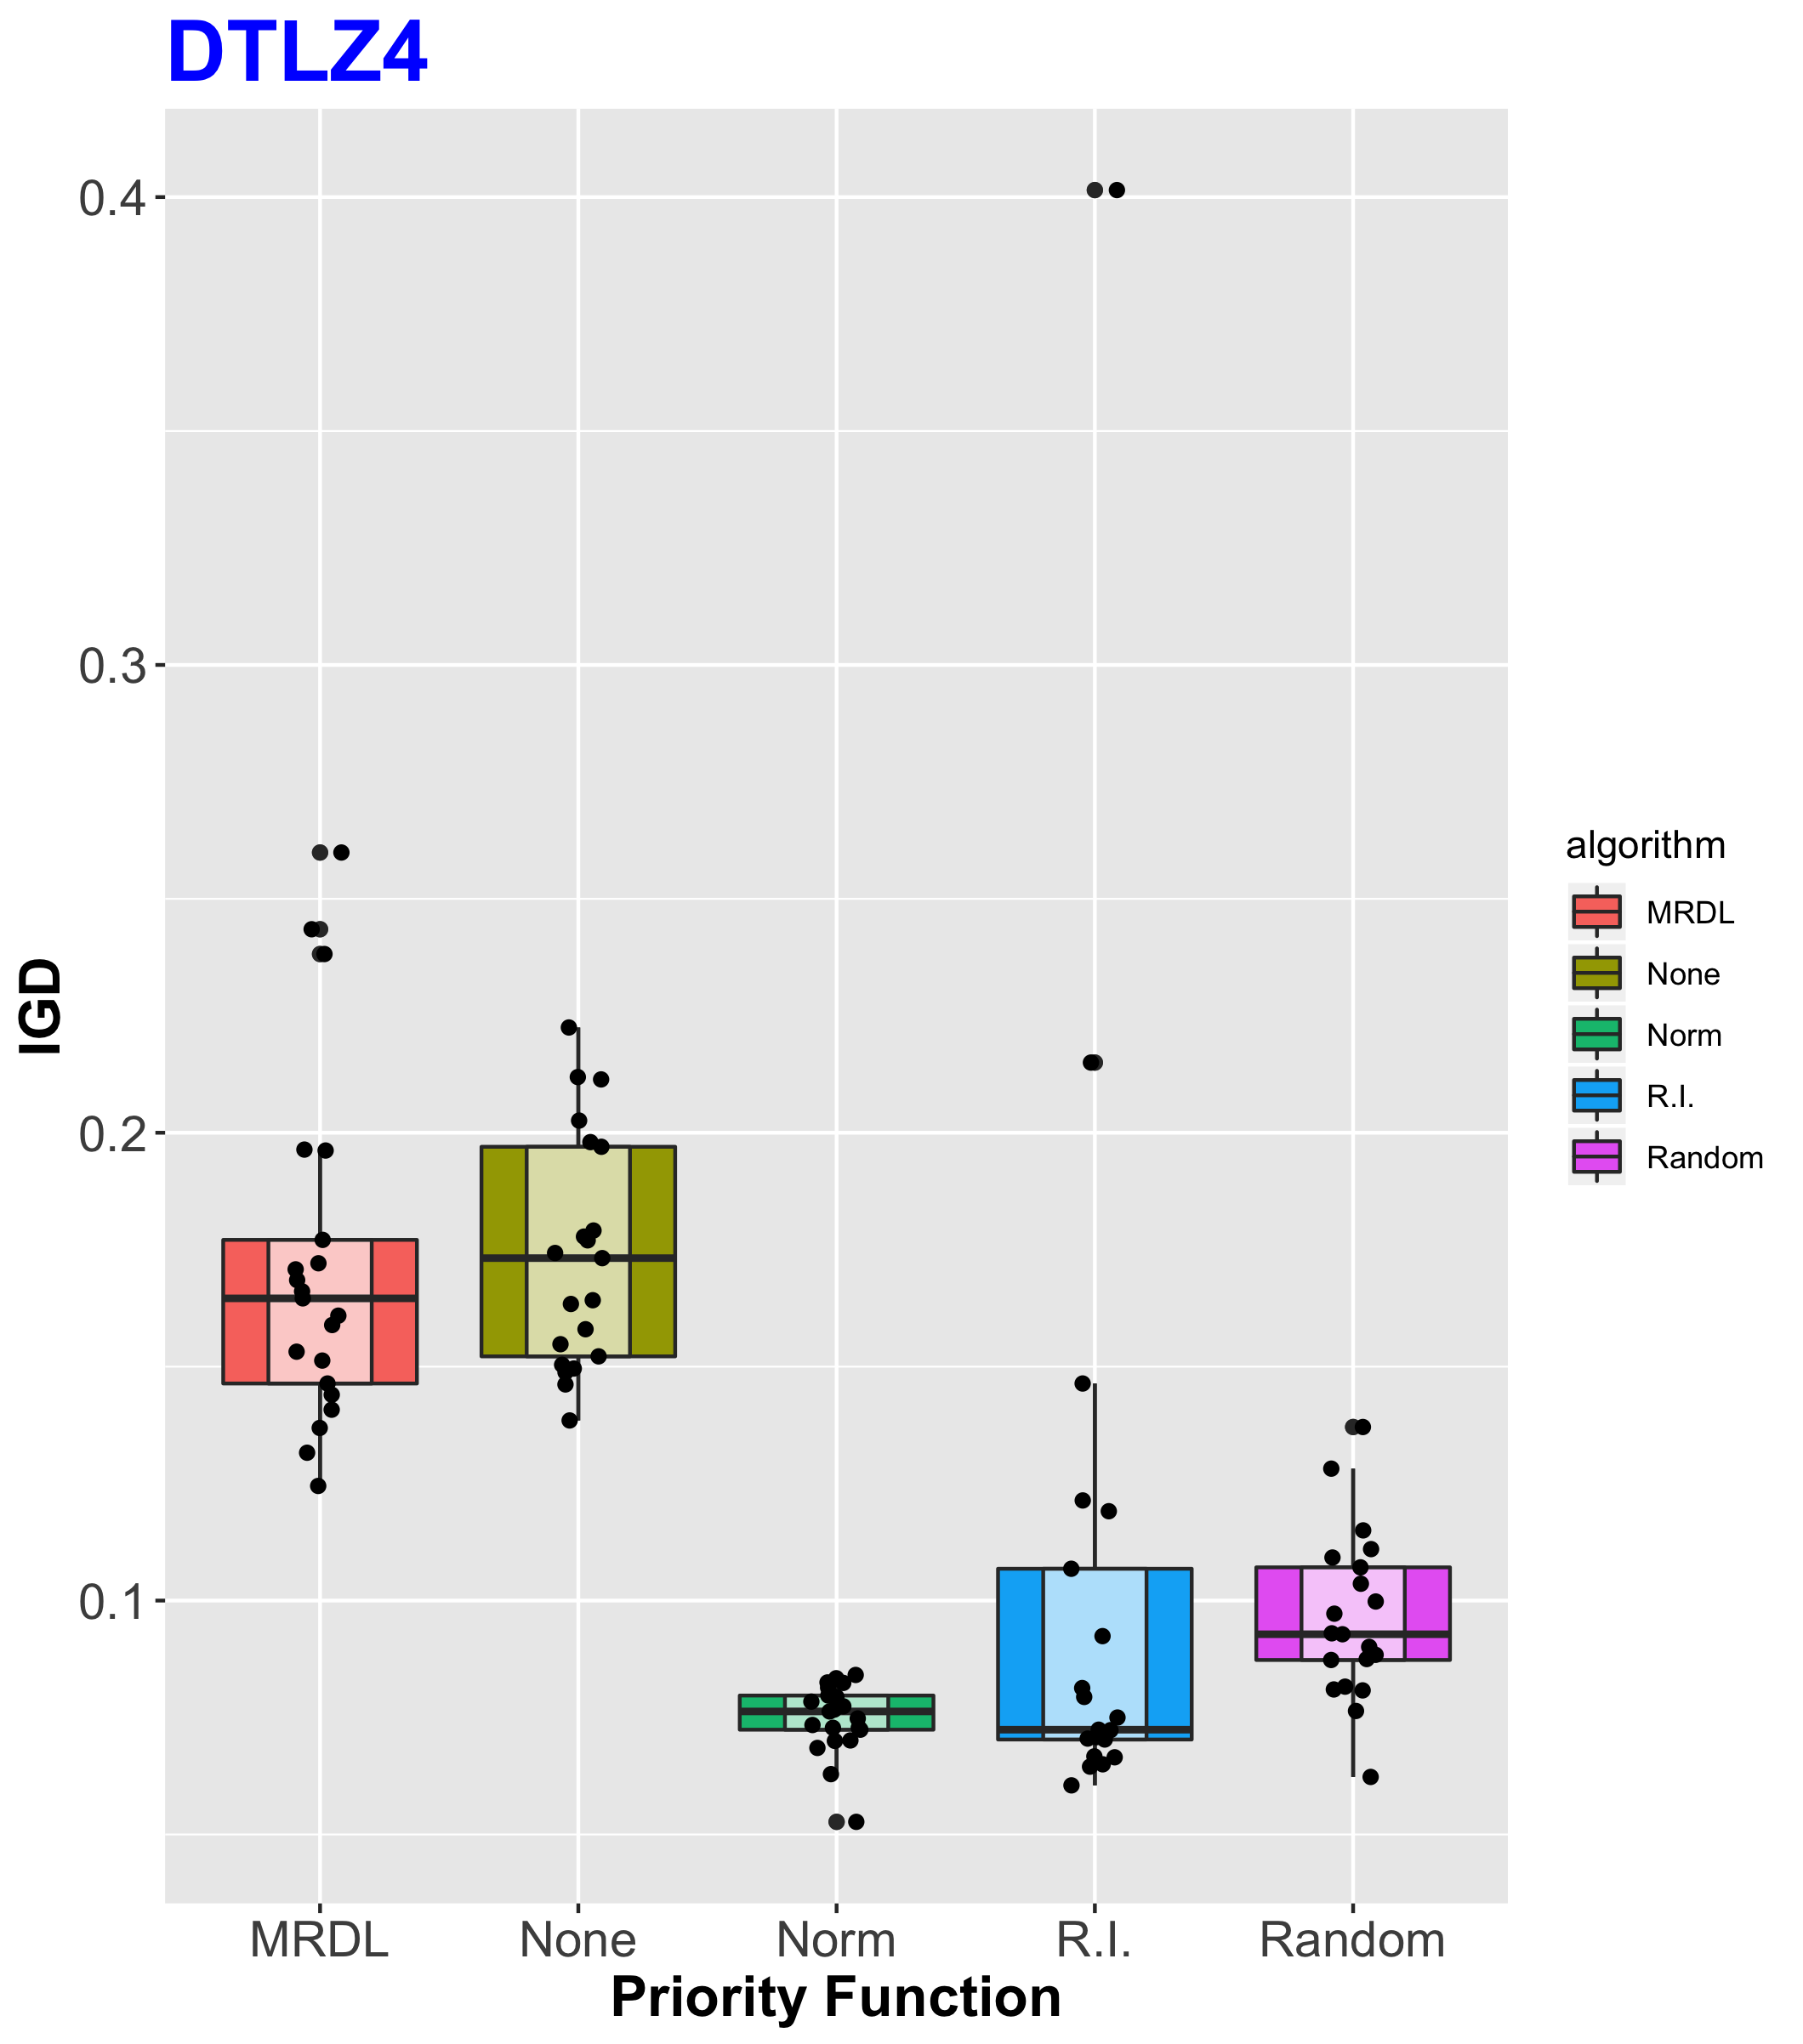
\includegraphics[width=1\textwidth, height=0.785\textwidth]{images/DTLZ4_IGD.png}
%	\caption{IGD - UF8}
	\end{subfigure}
%\begin{subfigure}[b]{0.33\textwidth}
%	\centering
%	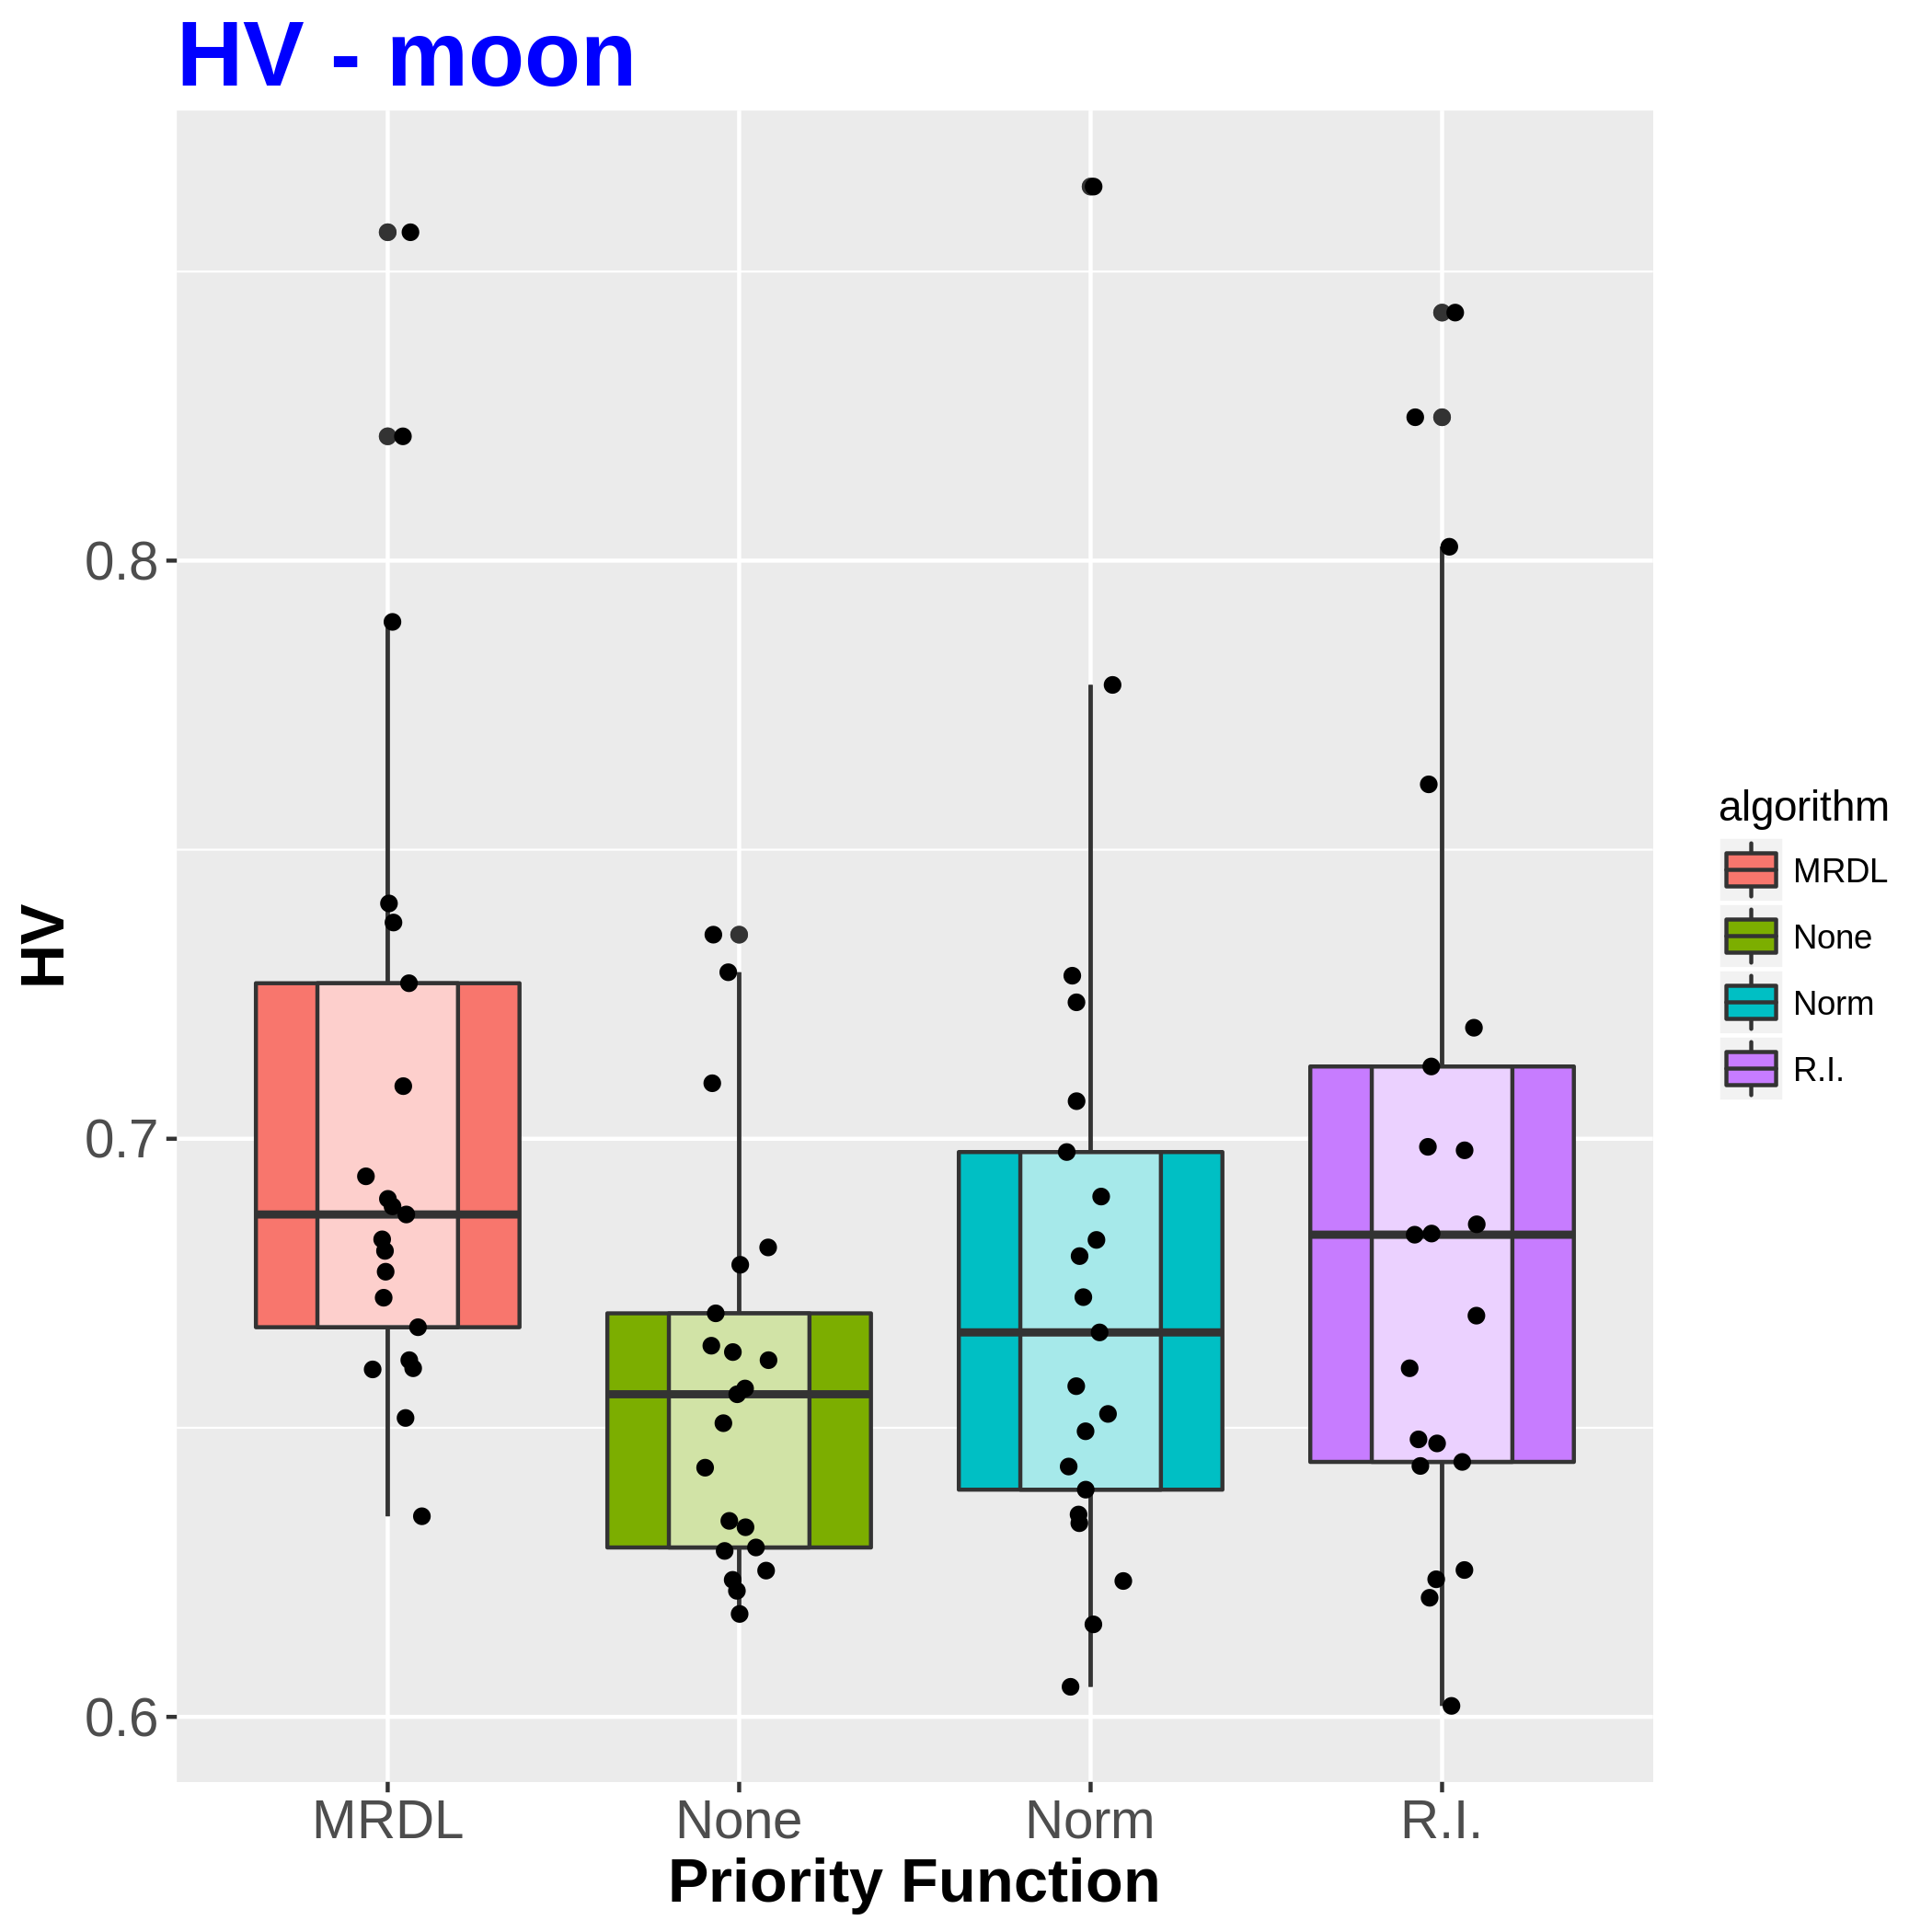
\includegraphics[width=1\textwidth, height=0.8\textwidth]{images/moon_HV}
%%	\caption{IGD - DTLZ4}
%\end{subfigure}
	\caption{Box plot of IGD values on UF9 and DTLZ4. None is the MOEA/D-DE with no priority function.}
		\label{IGDS}
\end{figure*}


%
%\begin{figure*}[!t]
%
%		\begin{subfigure}[b]{0.33\textwidth}
%			\centering
%		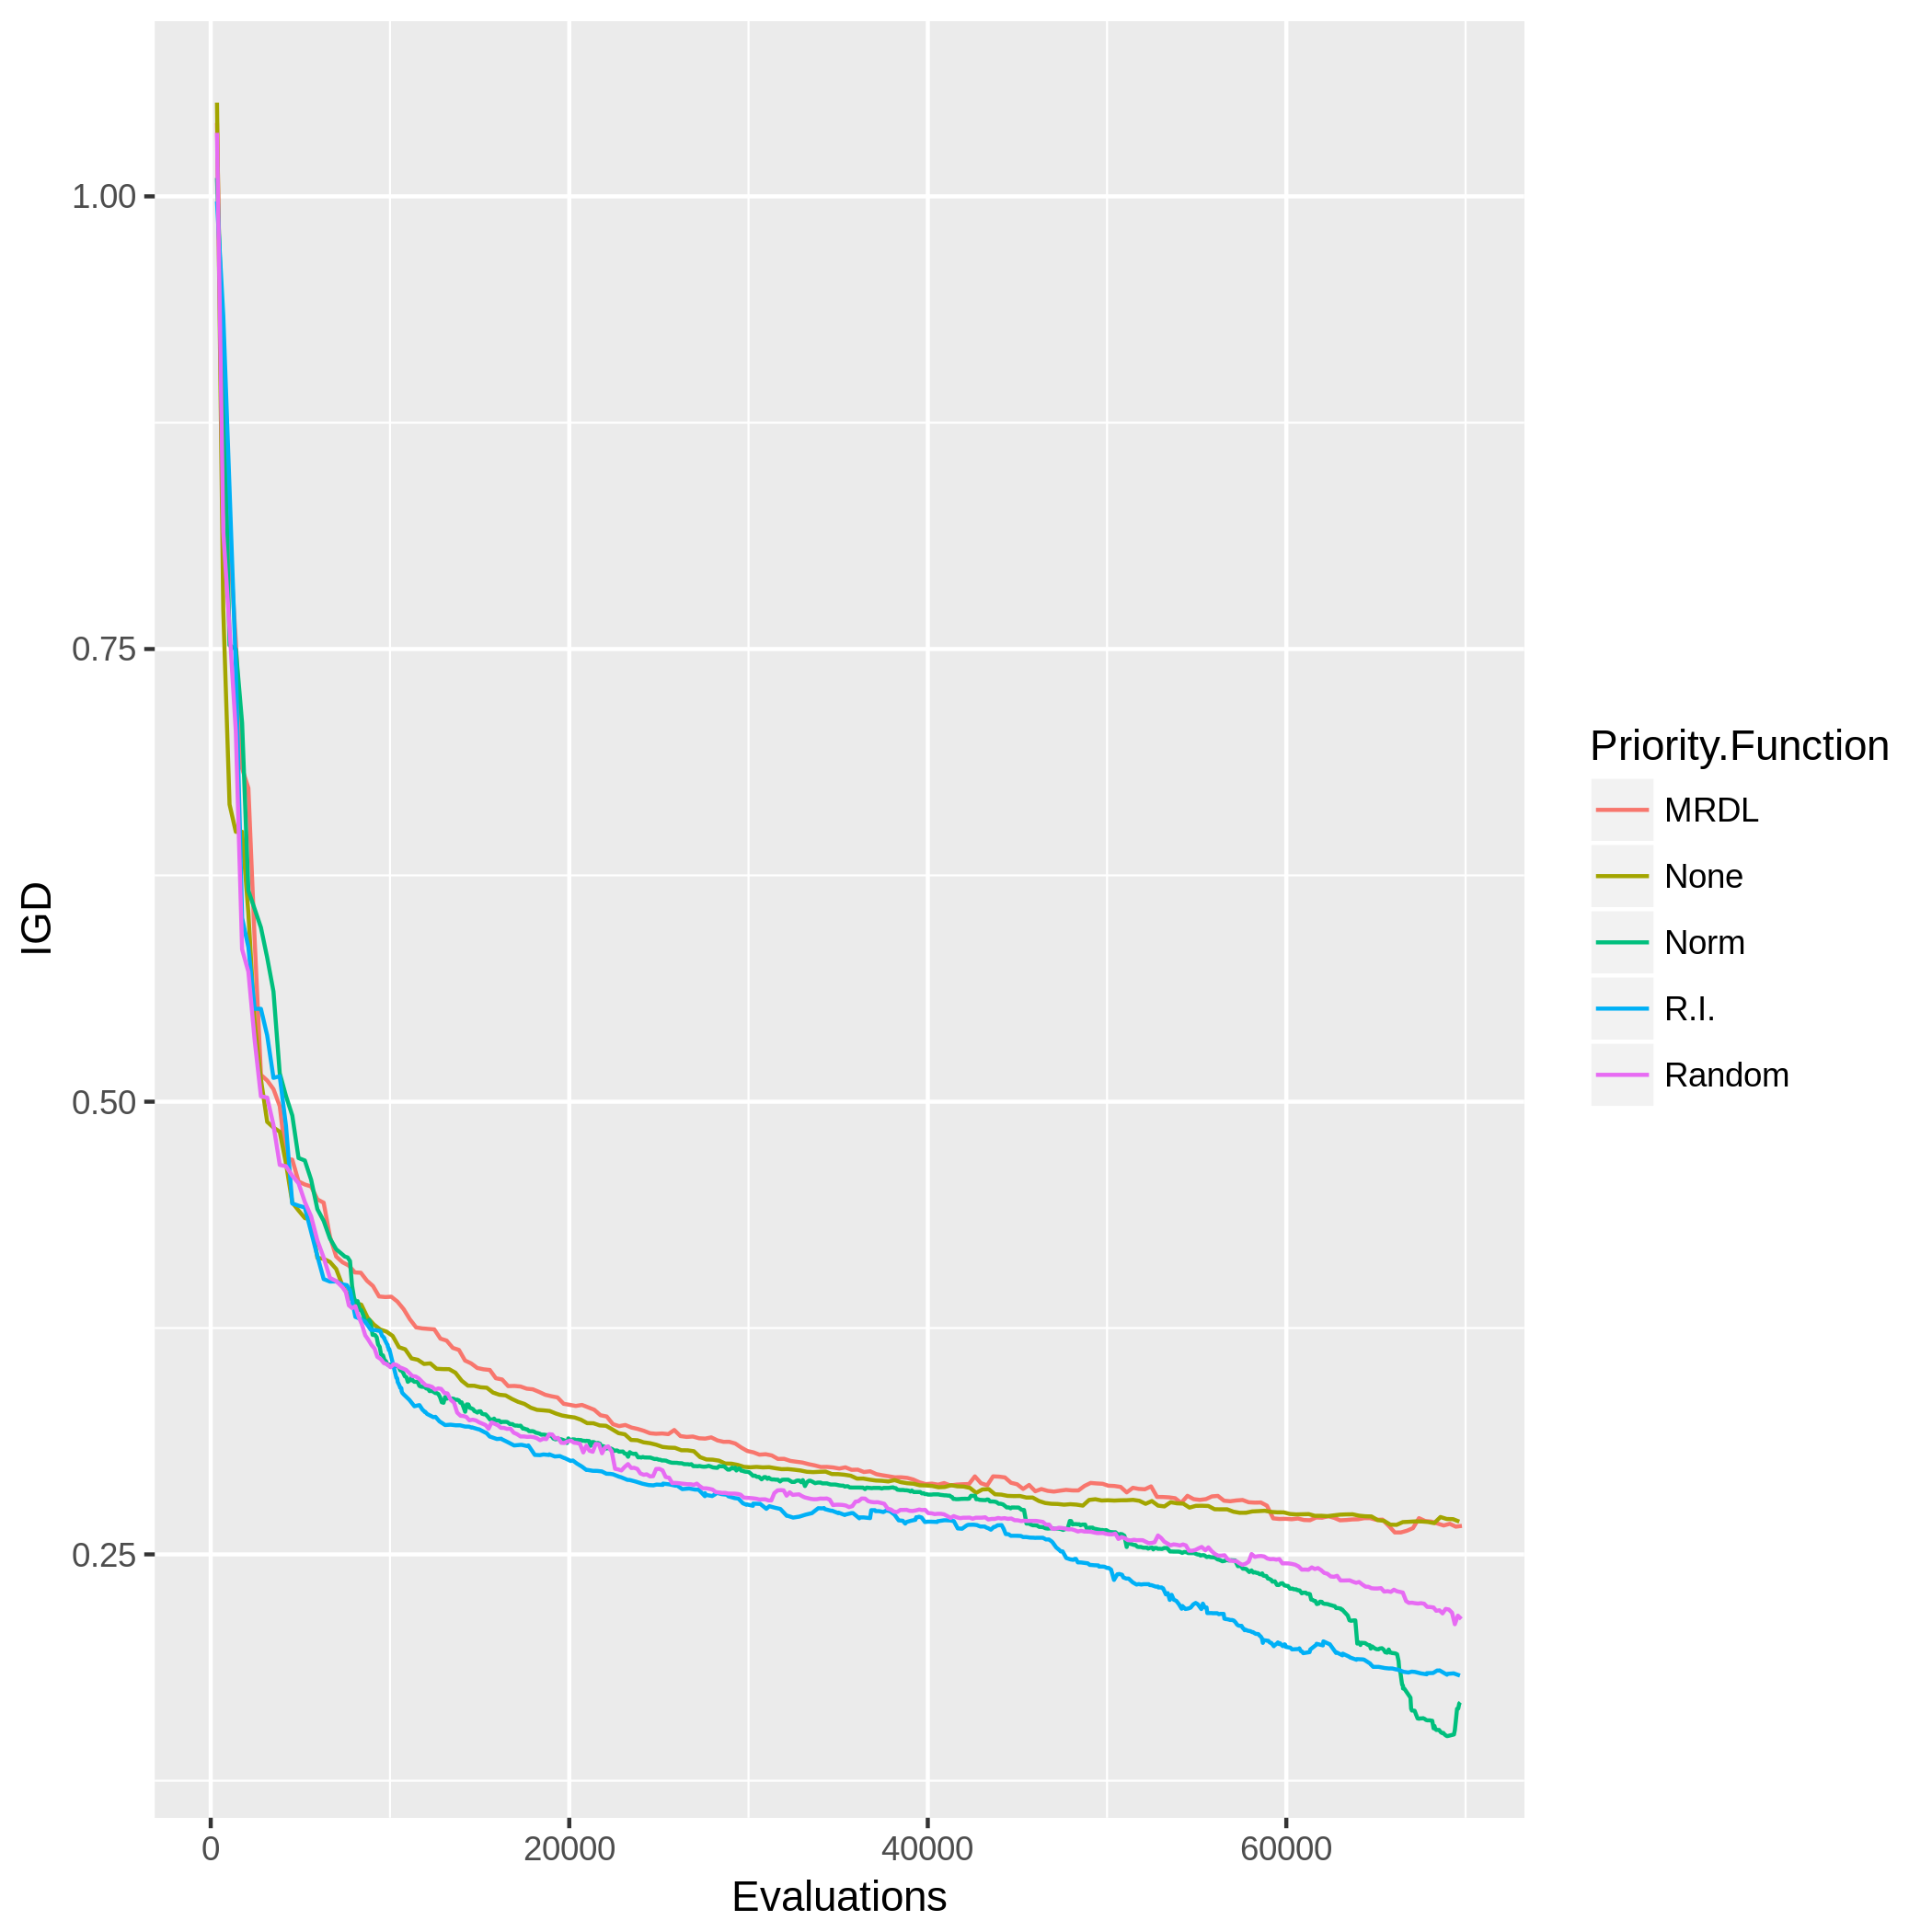
\includegraphics[width=1\textwidth, height=1\textwidth]{images/UF3igd_all}
%	\caption{Evolution - UF3}
%		\end{subfigure}
%		\begin{subfigure}[b]{0.33\textwidth}
%			\centering
%		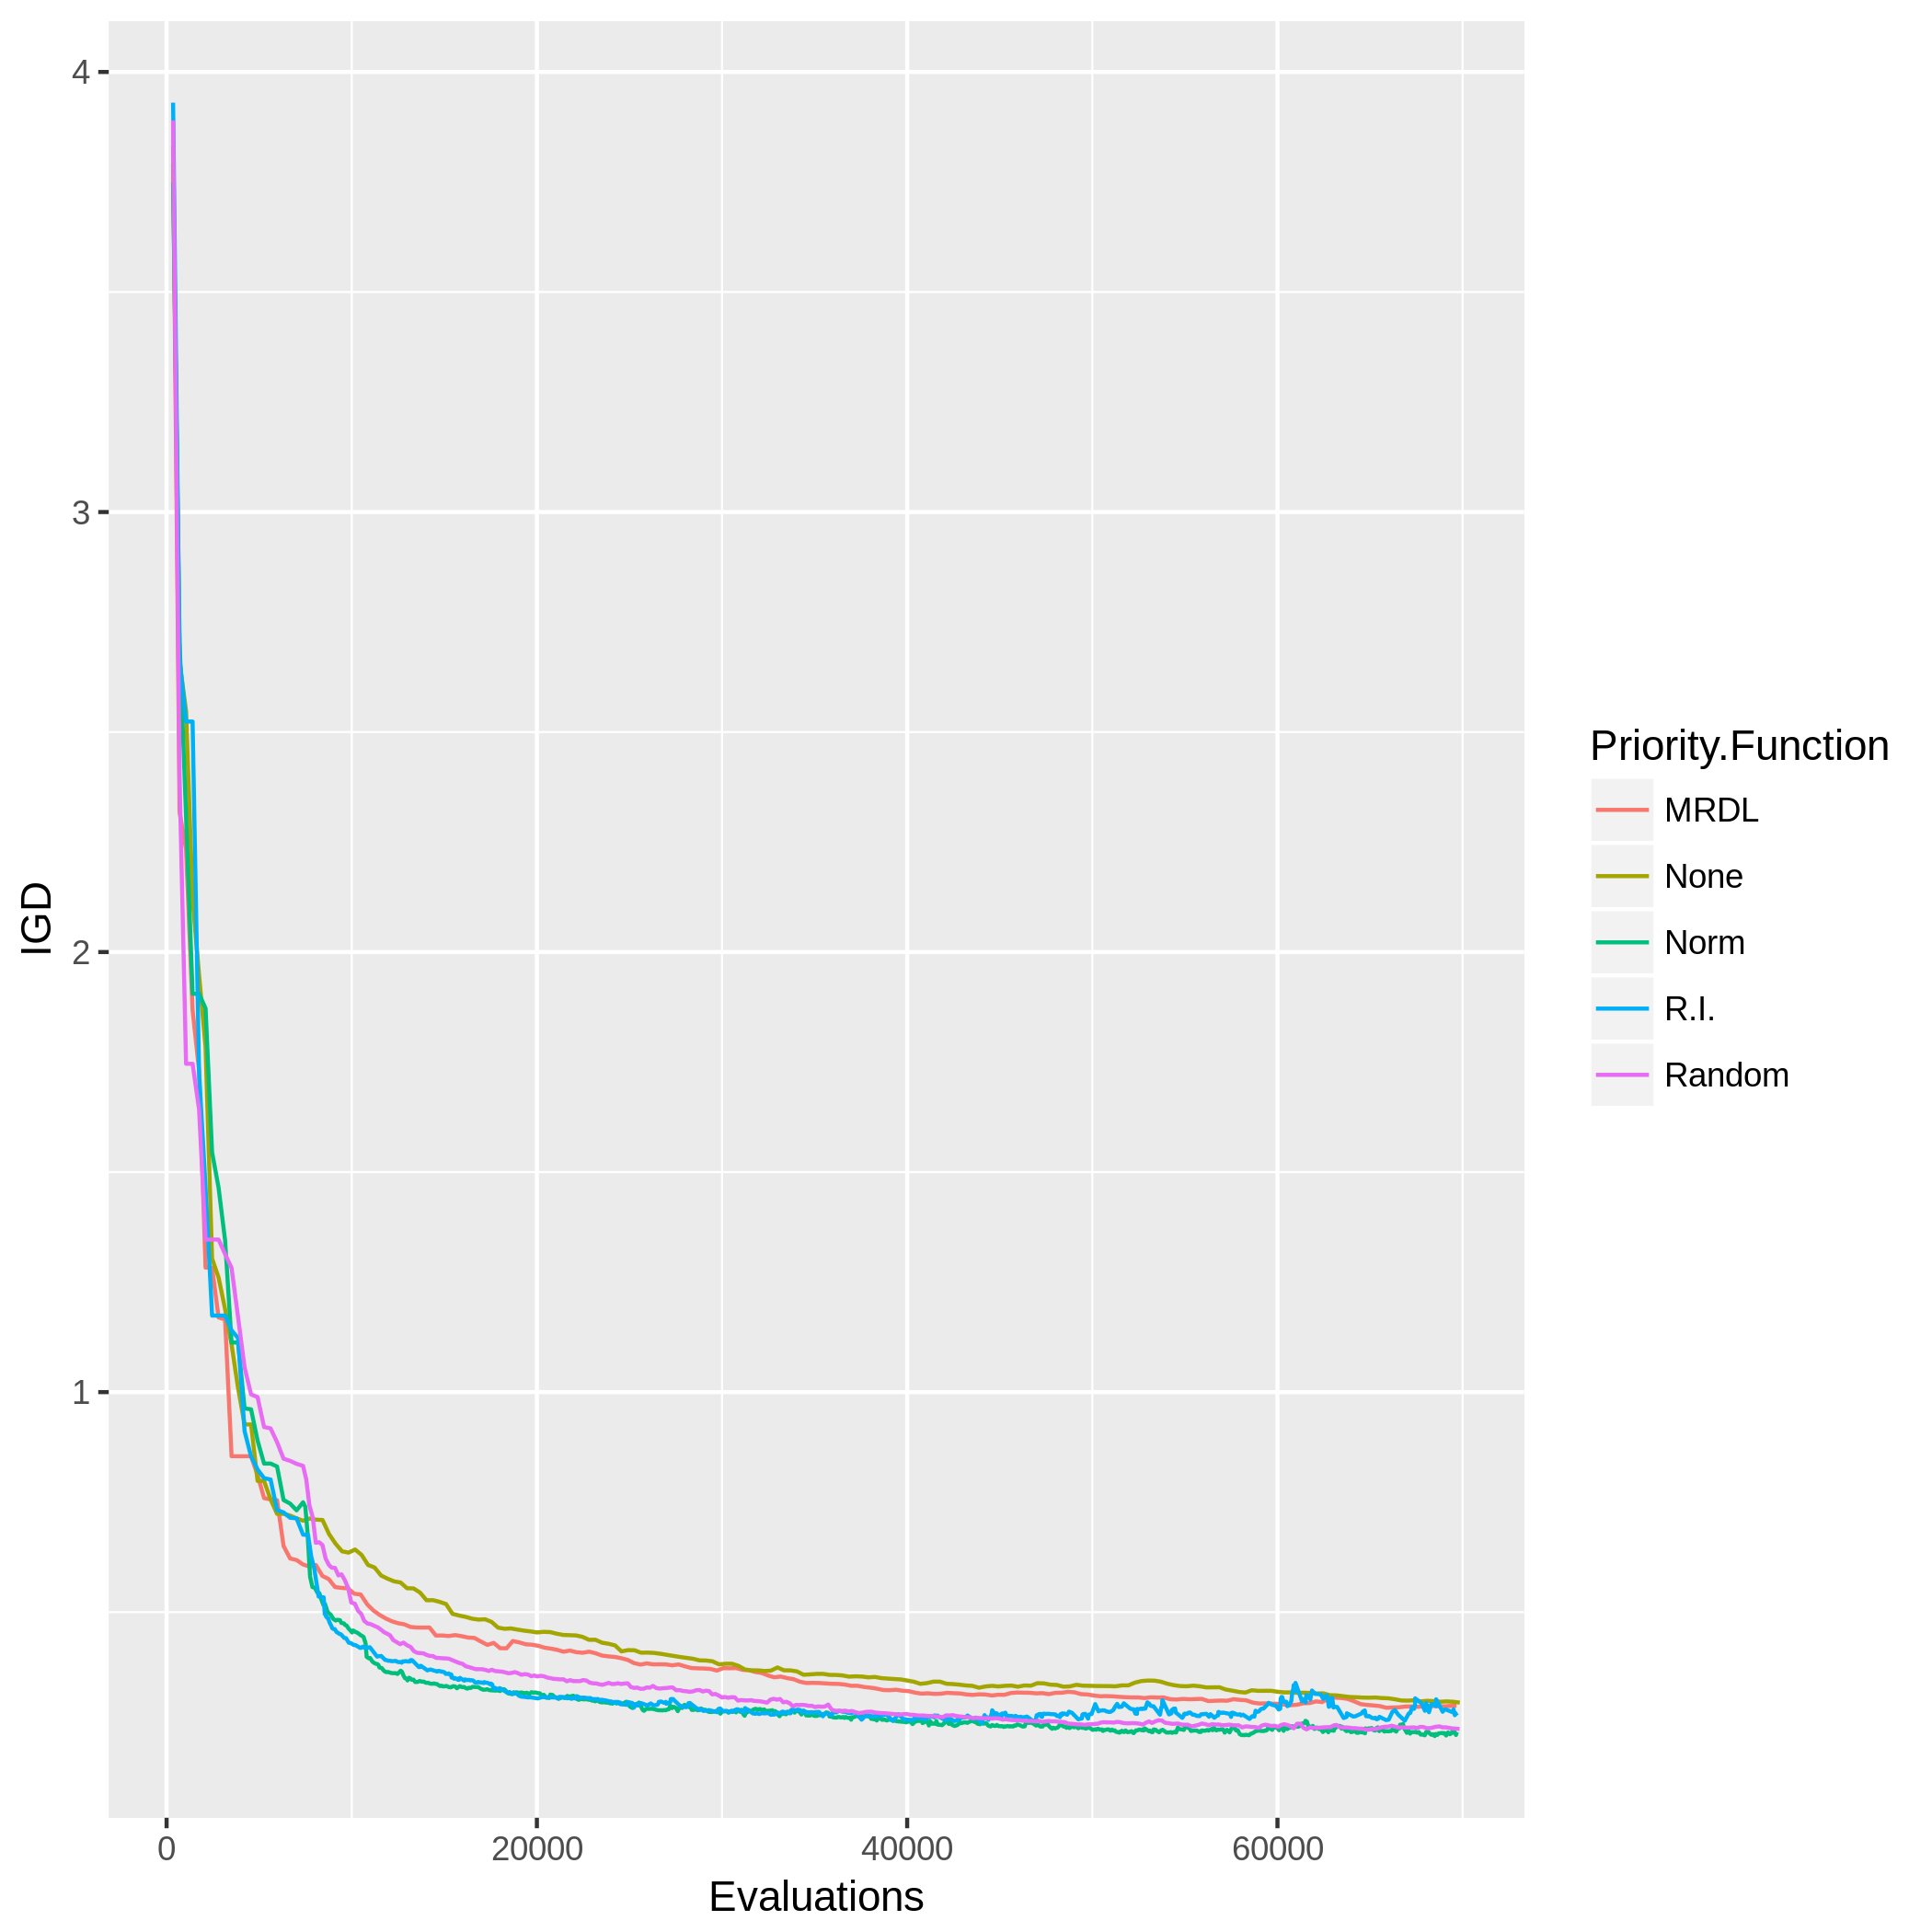
\includegraphics[width=1\textwidth, height=1\textwidth]{images/UF8igd_all}
%	\caption{Evolution - UF8}
%		\end{subfigure}
%	\begin{subfigure}[b]{0.33\textwidth}
%		\centering
%		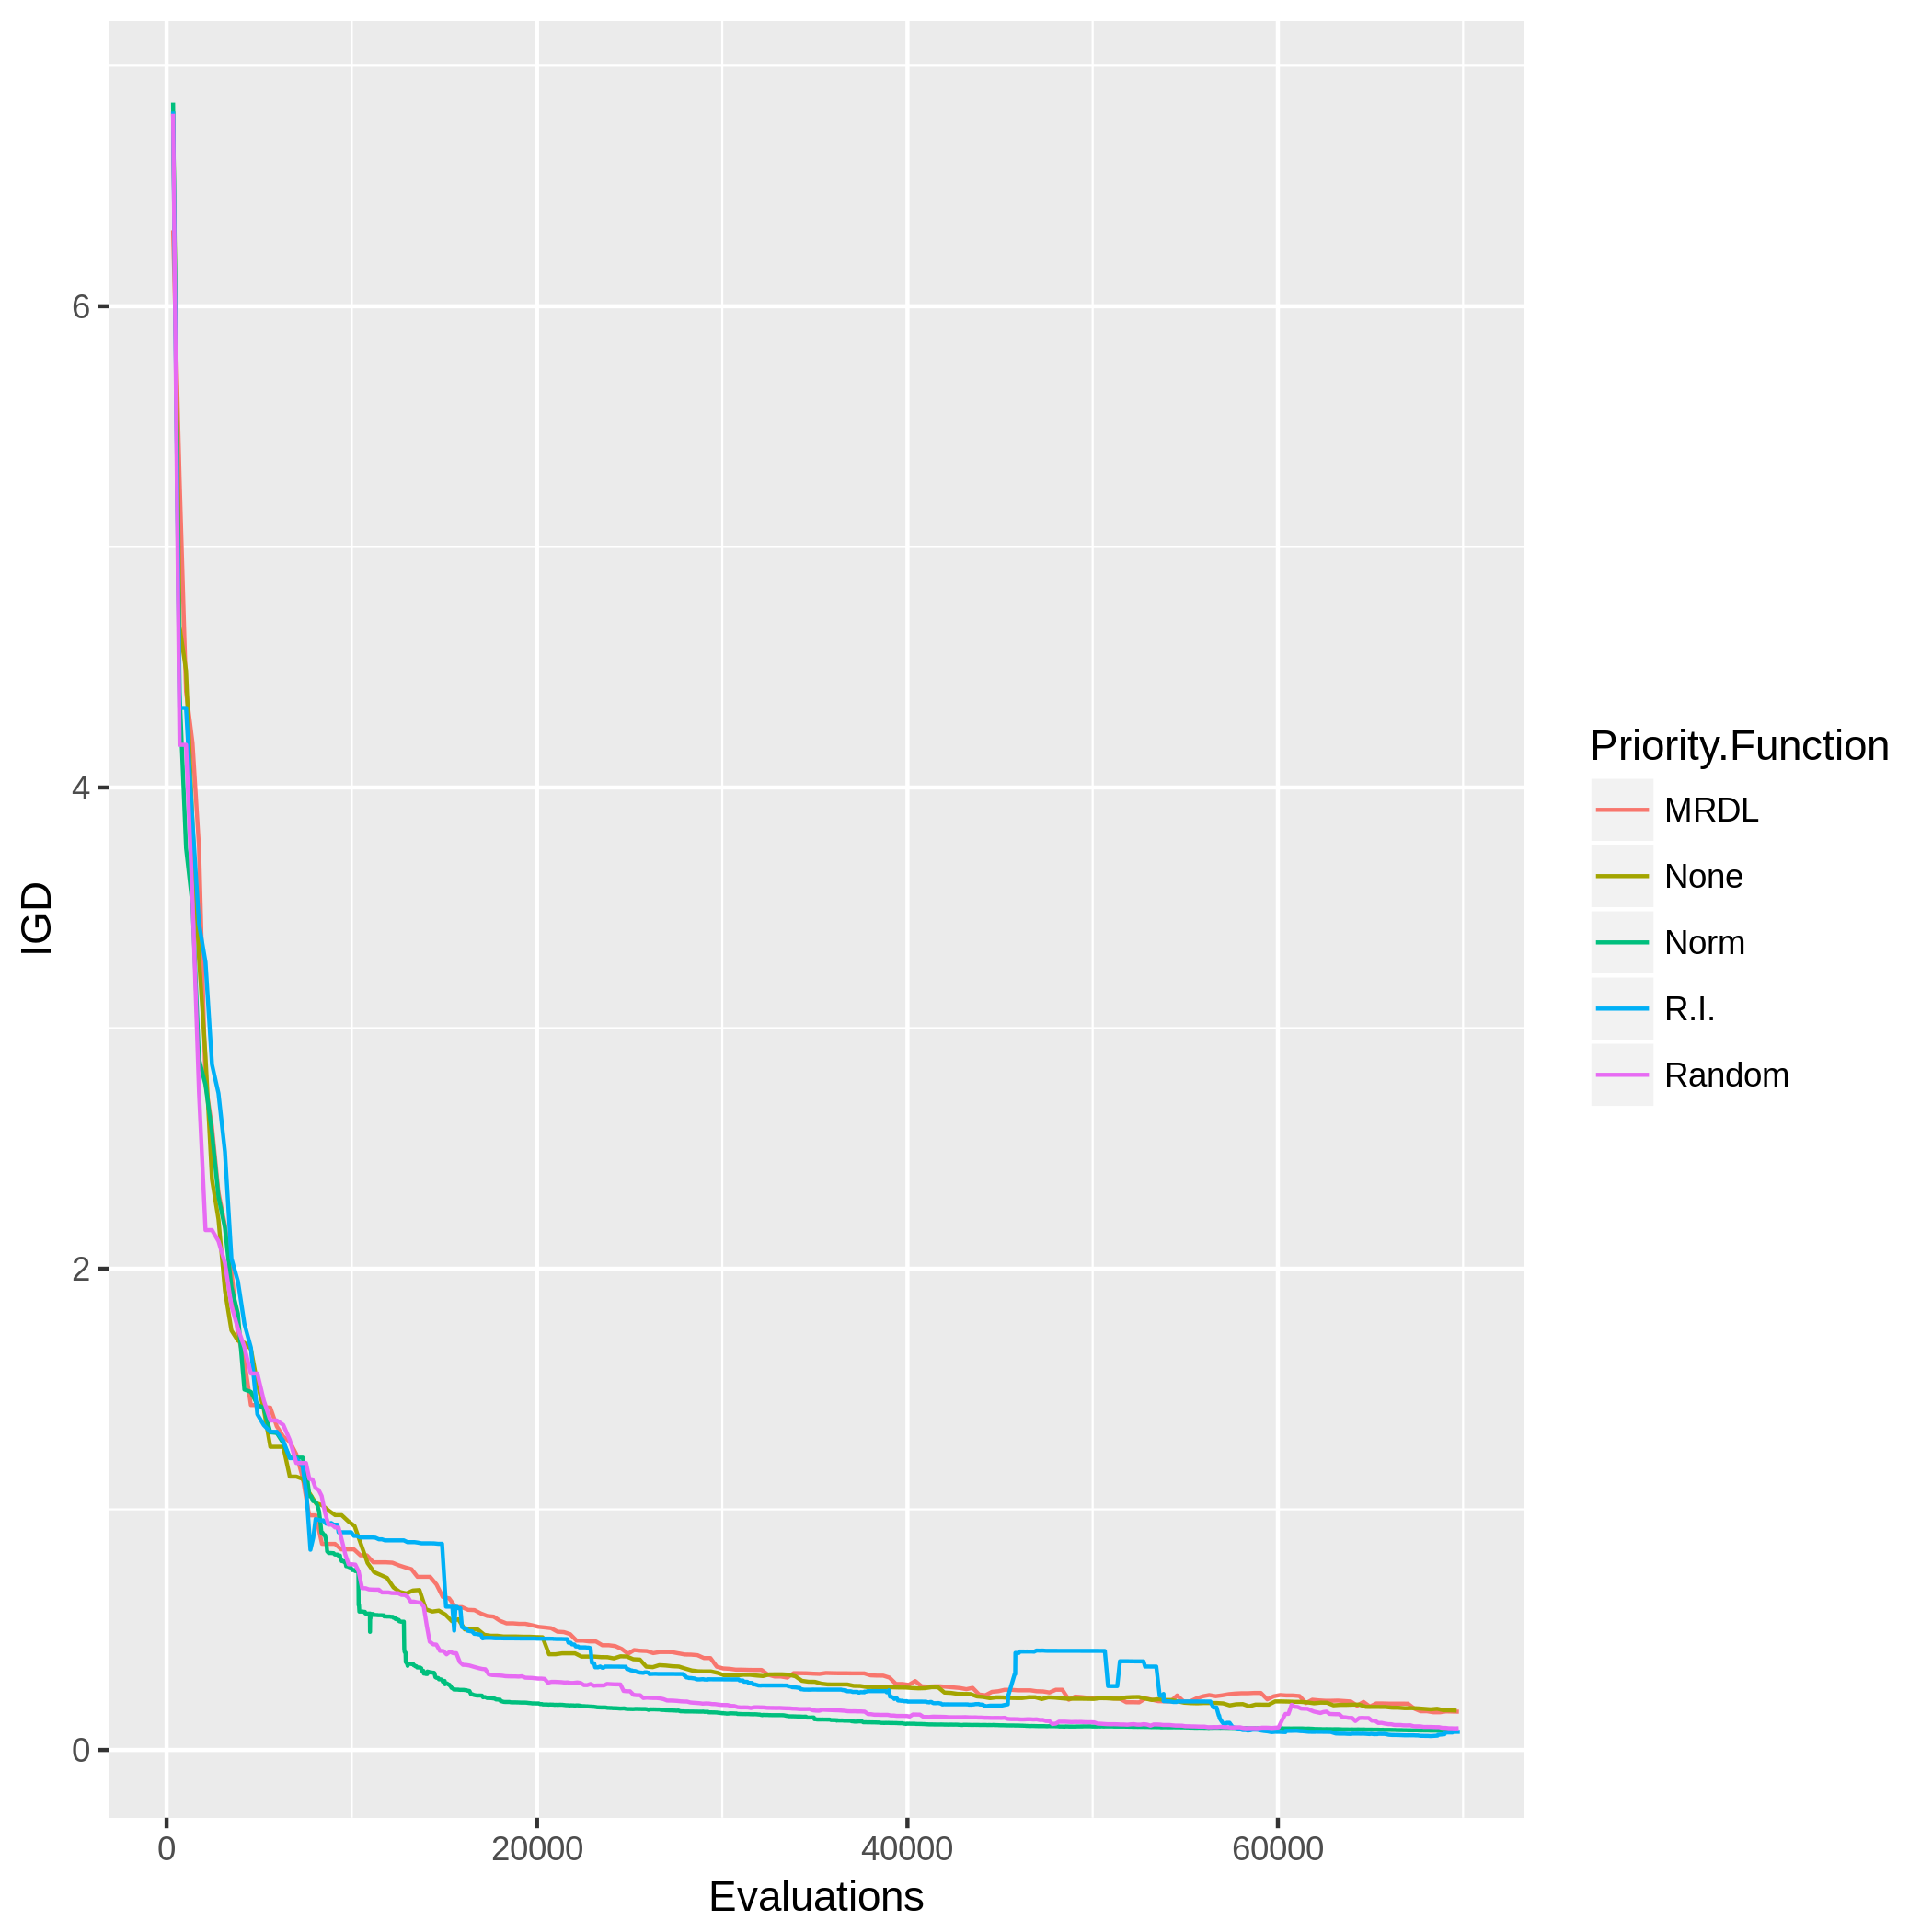
\includegraphics[width=1\textwidth, height=1\textwidth]{images/DTLZ4igd_all}
%	\caption{Evolution - DTLZ4}
%	\end{subfigure}
%	\caption{Evolution of HV values on Artificial Benchmark Problems}
%			\label{evolution_igd}
%	\end{figure*}

\begin{figure}[!t]

	%	\Large{Average performance on different tournament size - Gallagher's Gaussian 21-hi Peaks Function}
	%	\begin{subfigure}[b]{0.33\textwidth}
	\centering
	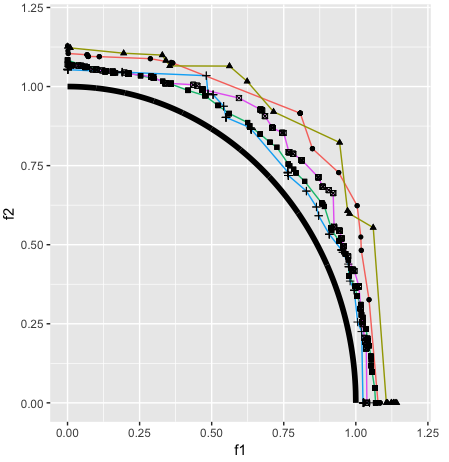
\includegraphics[width=0.45\textwidth, height=0.33\textwidth]{images/Pareto-front-dtlz4.png}
	%		\caption{RA- UF8}
	%	\end{subfigure}
	\caption{Pareto Front approximations of all priority functions and MOEA/D-DE (None).}
	\label{PFs}

\end{figure}

\begin{figure*}[!t]

	%	\Large{Average performance on different tournament size - Gallagher's Gaussian 21-hi Peaks Function}
	\begin{subfigure}[b]{0.33\textwidth}
		\centering
		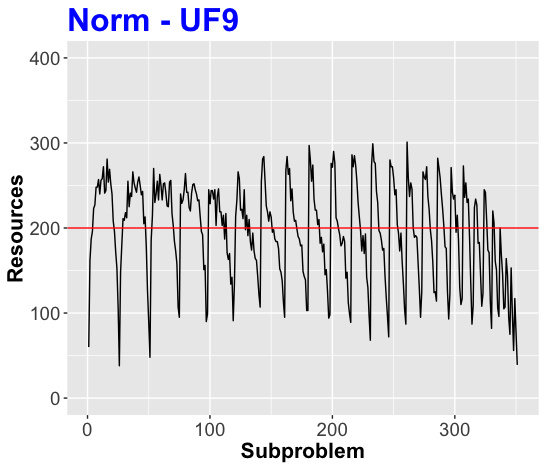
\includegraphics[width=1\textwidth, height=0.8\textwidth]{images/Ra-norm-uf9.png}
%		\caption{RA- UF8}
	\end{subfigure}
	\begin{subfigure}[b]{0.33\textwidth}
		\centering
		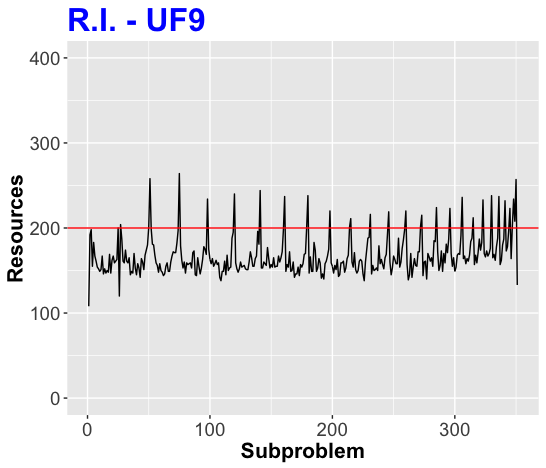
\includegraphics[width=1\textwidth, height=0.8\textwidth]{images/Ra-gra-uf9.png}
%		\caption{RA- UF8}
	\end{subfigure}
	\begin{subfigure}[b]{0.33\textwidth}
		\centering
		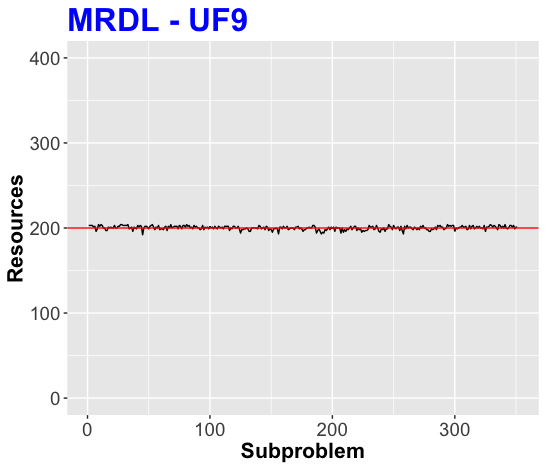
\includegraphics[width=1\textwidth, height=0.8\textwidth]{images/Ra-mrdl-uf9.png}
%		\caption{RA- UF8}
	\end{subfigure}
	\begin{subfigure}[b]{0.33\textwidth}
		\centering
		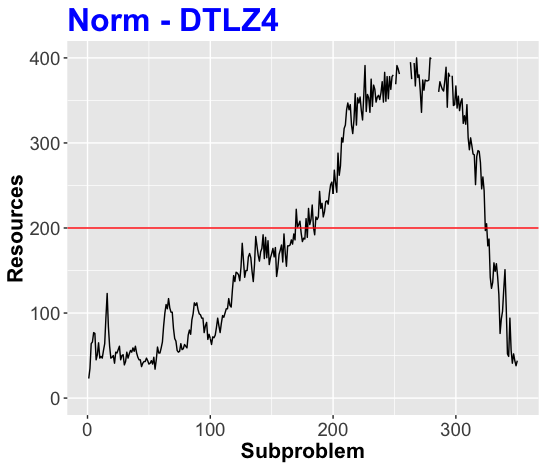
\includegraphics[width=1\textwidth, height=0.8\textwidth]{images/Ra-norm-dtlz4.png}
%		\caption{RA- UF8}
	\end{subfigure}
	\begin{subfigure}[b]{0.33\textwidth}
		\centering
		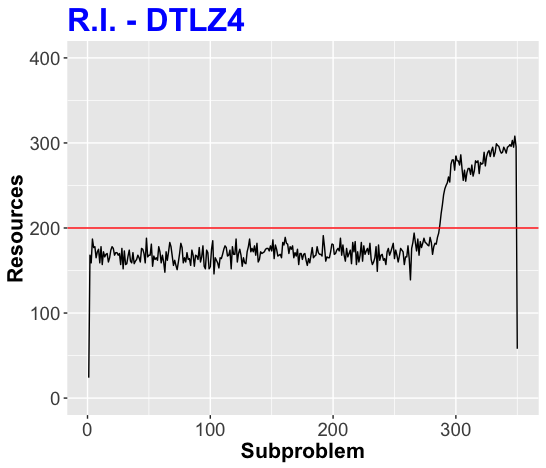
\includegraphics[width=1\textwidth, height=0.8\textwidth]{images/Ra-gra-dtlz4.png}
%		\caption{RA- UF8}
	\end{subfigure}
	\begin{subfigure}[b]{0.33\textwidth}
		\centering
		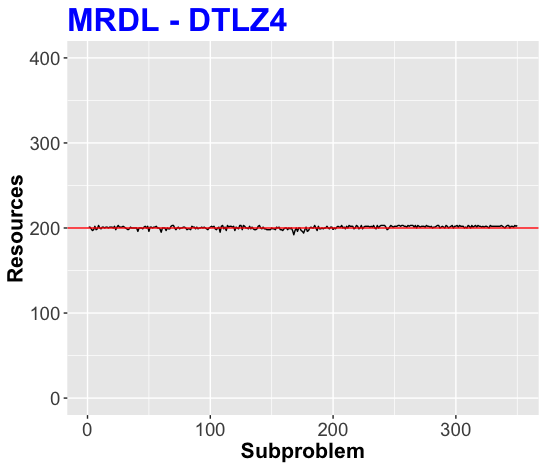
\includegraphics[width=1\textwidth, height=0.8\textwidth]{images/Ra-mrdl-dtlz4.png}
%		\caption{RA- UF8}
	\end{subfigure}
	\caption{Resource allocation by subproblem - The red line indicates the default amount of resource for each problem, i.e., with no priority function.}
	\label{RAs}

\end{figure*}



%
%\begin{figure*}[!t]
%
%	%	\Large{Average performance on different tournament size - Gallagher's Gaussian 21-hi Peaks Function}
%	\begin{subfigure}[b]{0.33\textwidth}
%		\centering
%		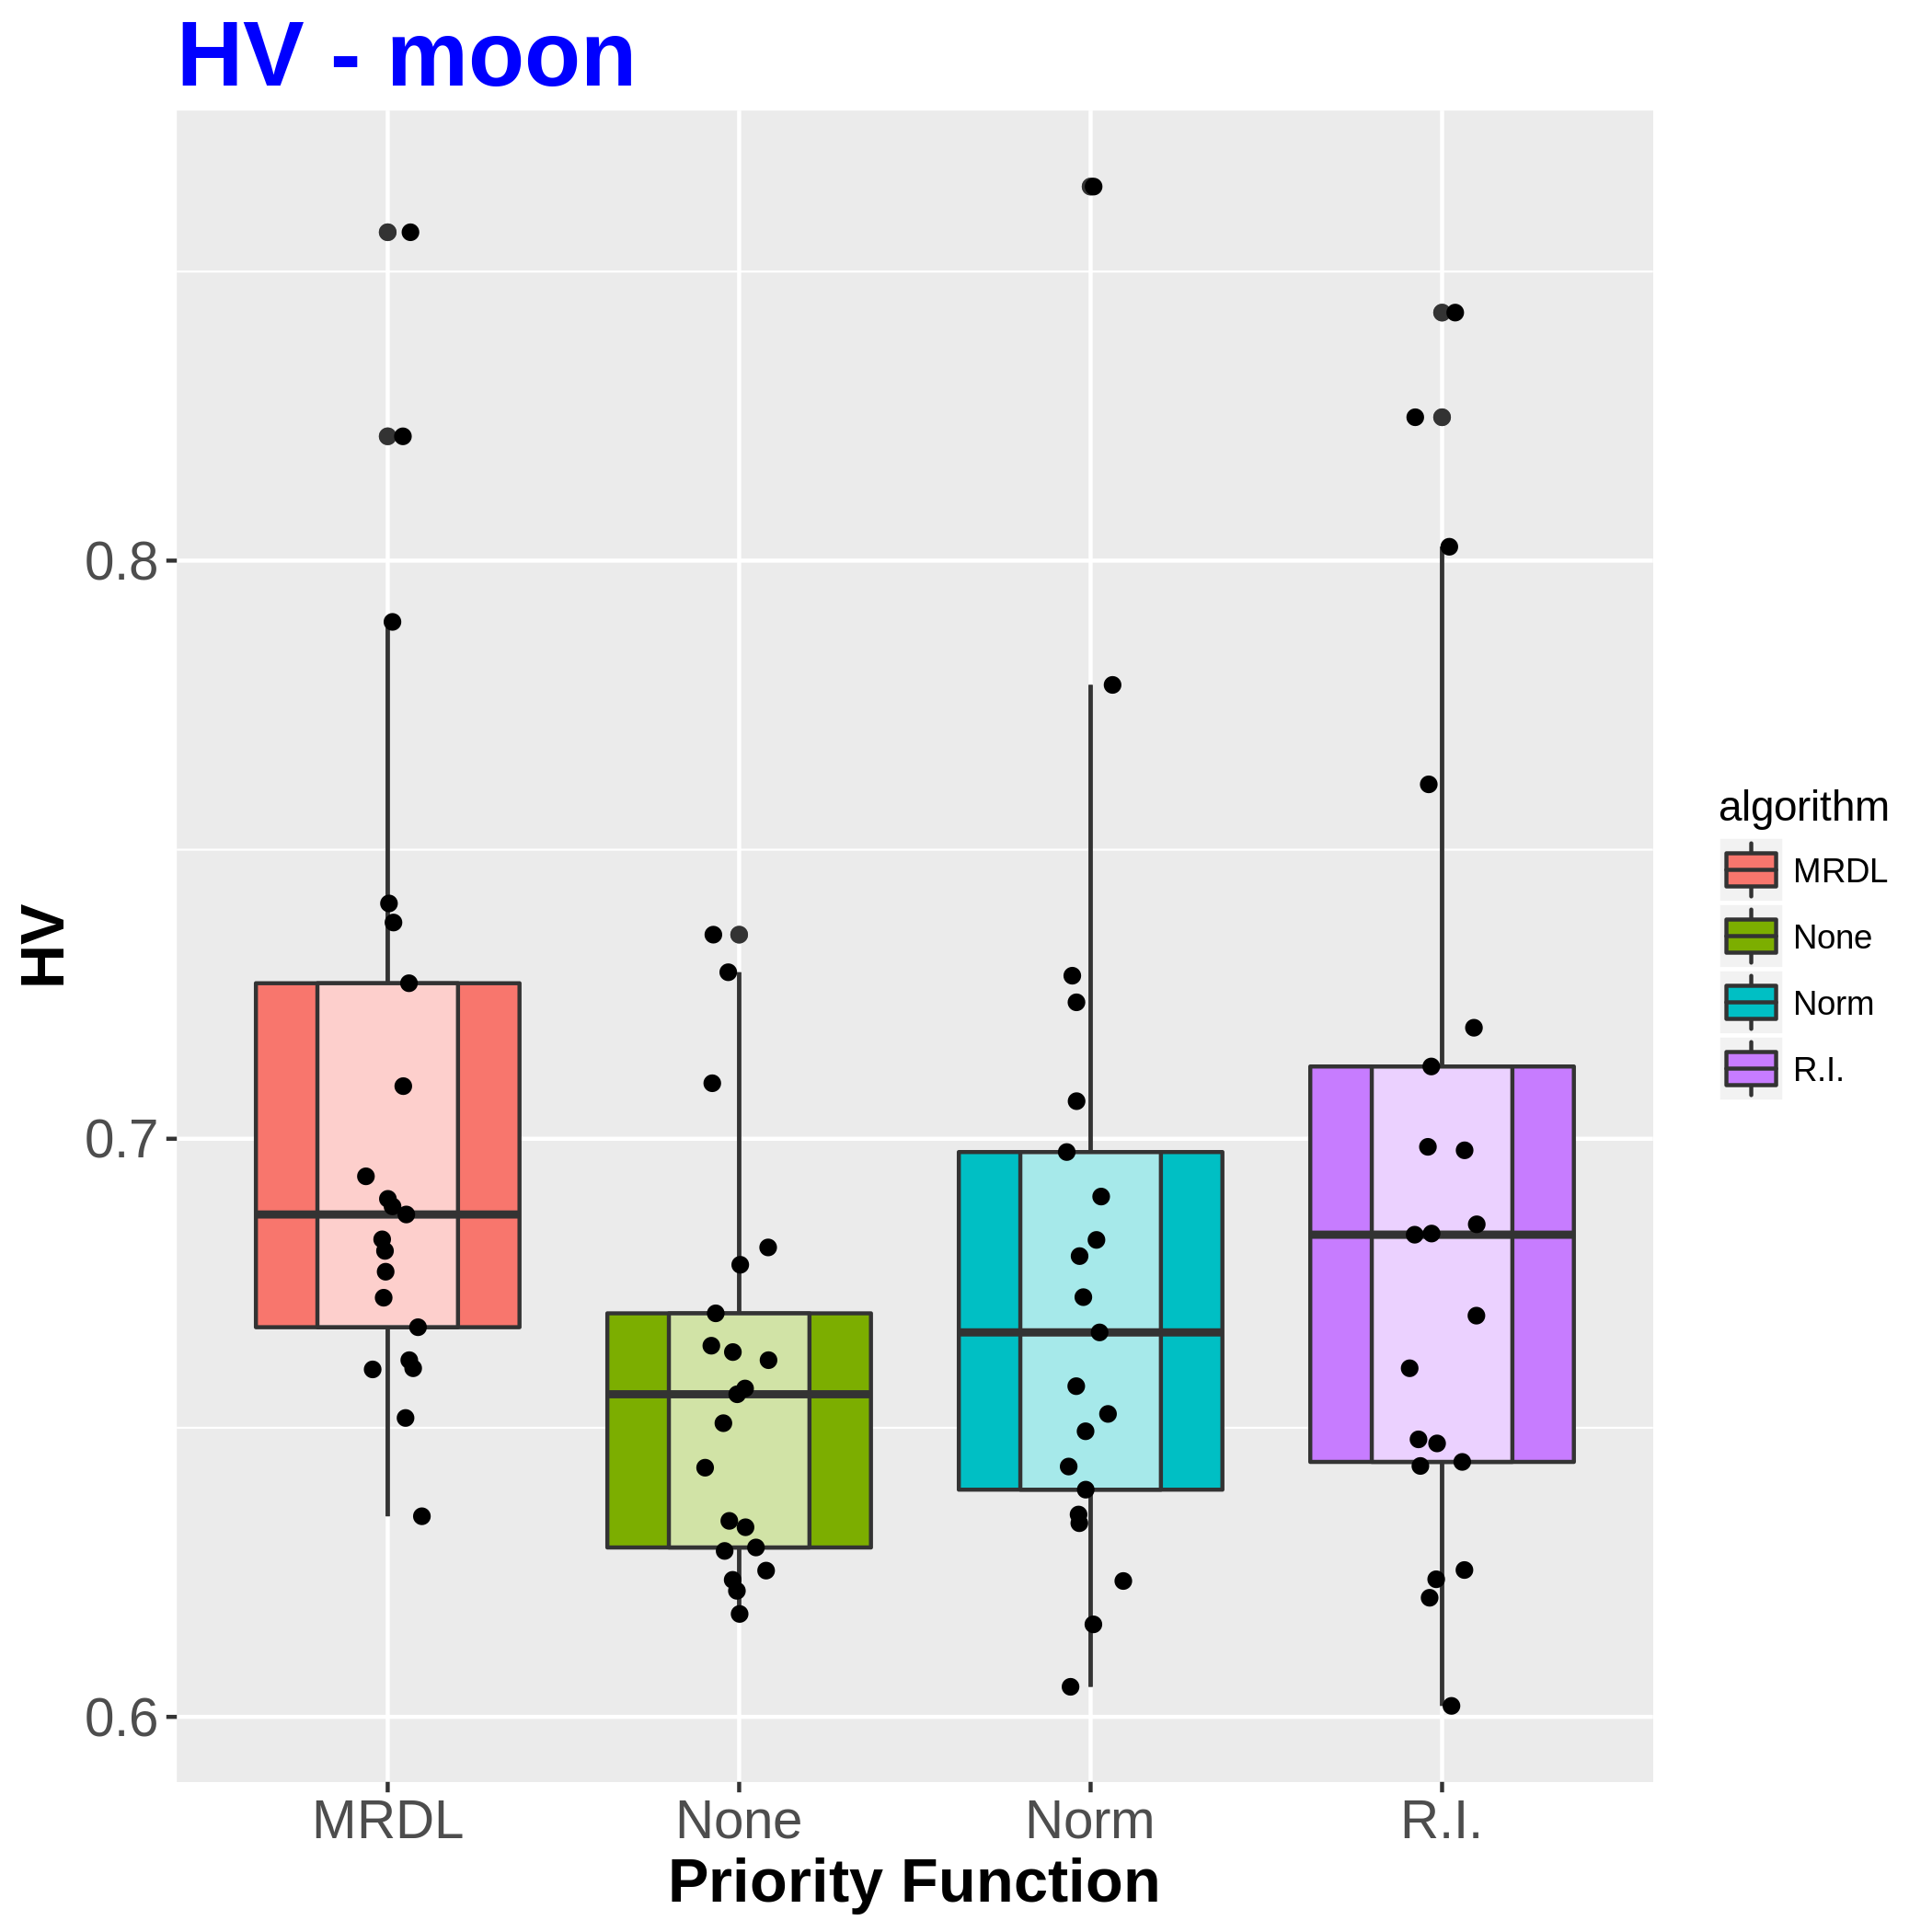
\includegraphics[width=1\textwidth, height=1\textwidth]{images/moon_HV}
%		\caption{HV values of the last iteraction on the Lunar Landing Problem}
%	\end{subfigure}
%%	\begin{subfigure}[b]{0.33\textwidth}
%%		\centering
%%		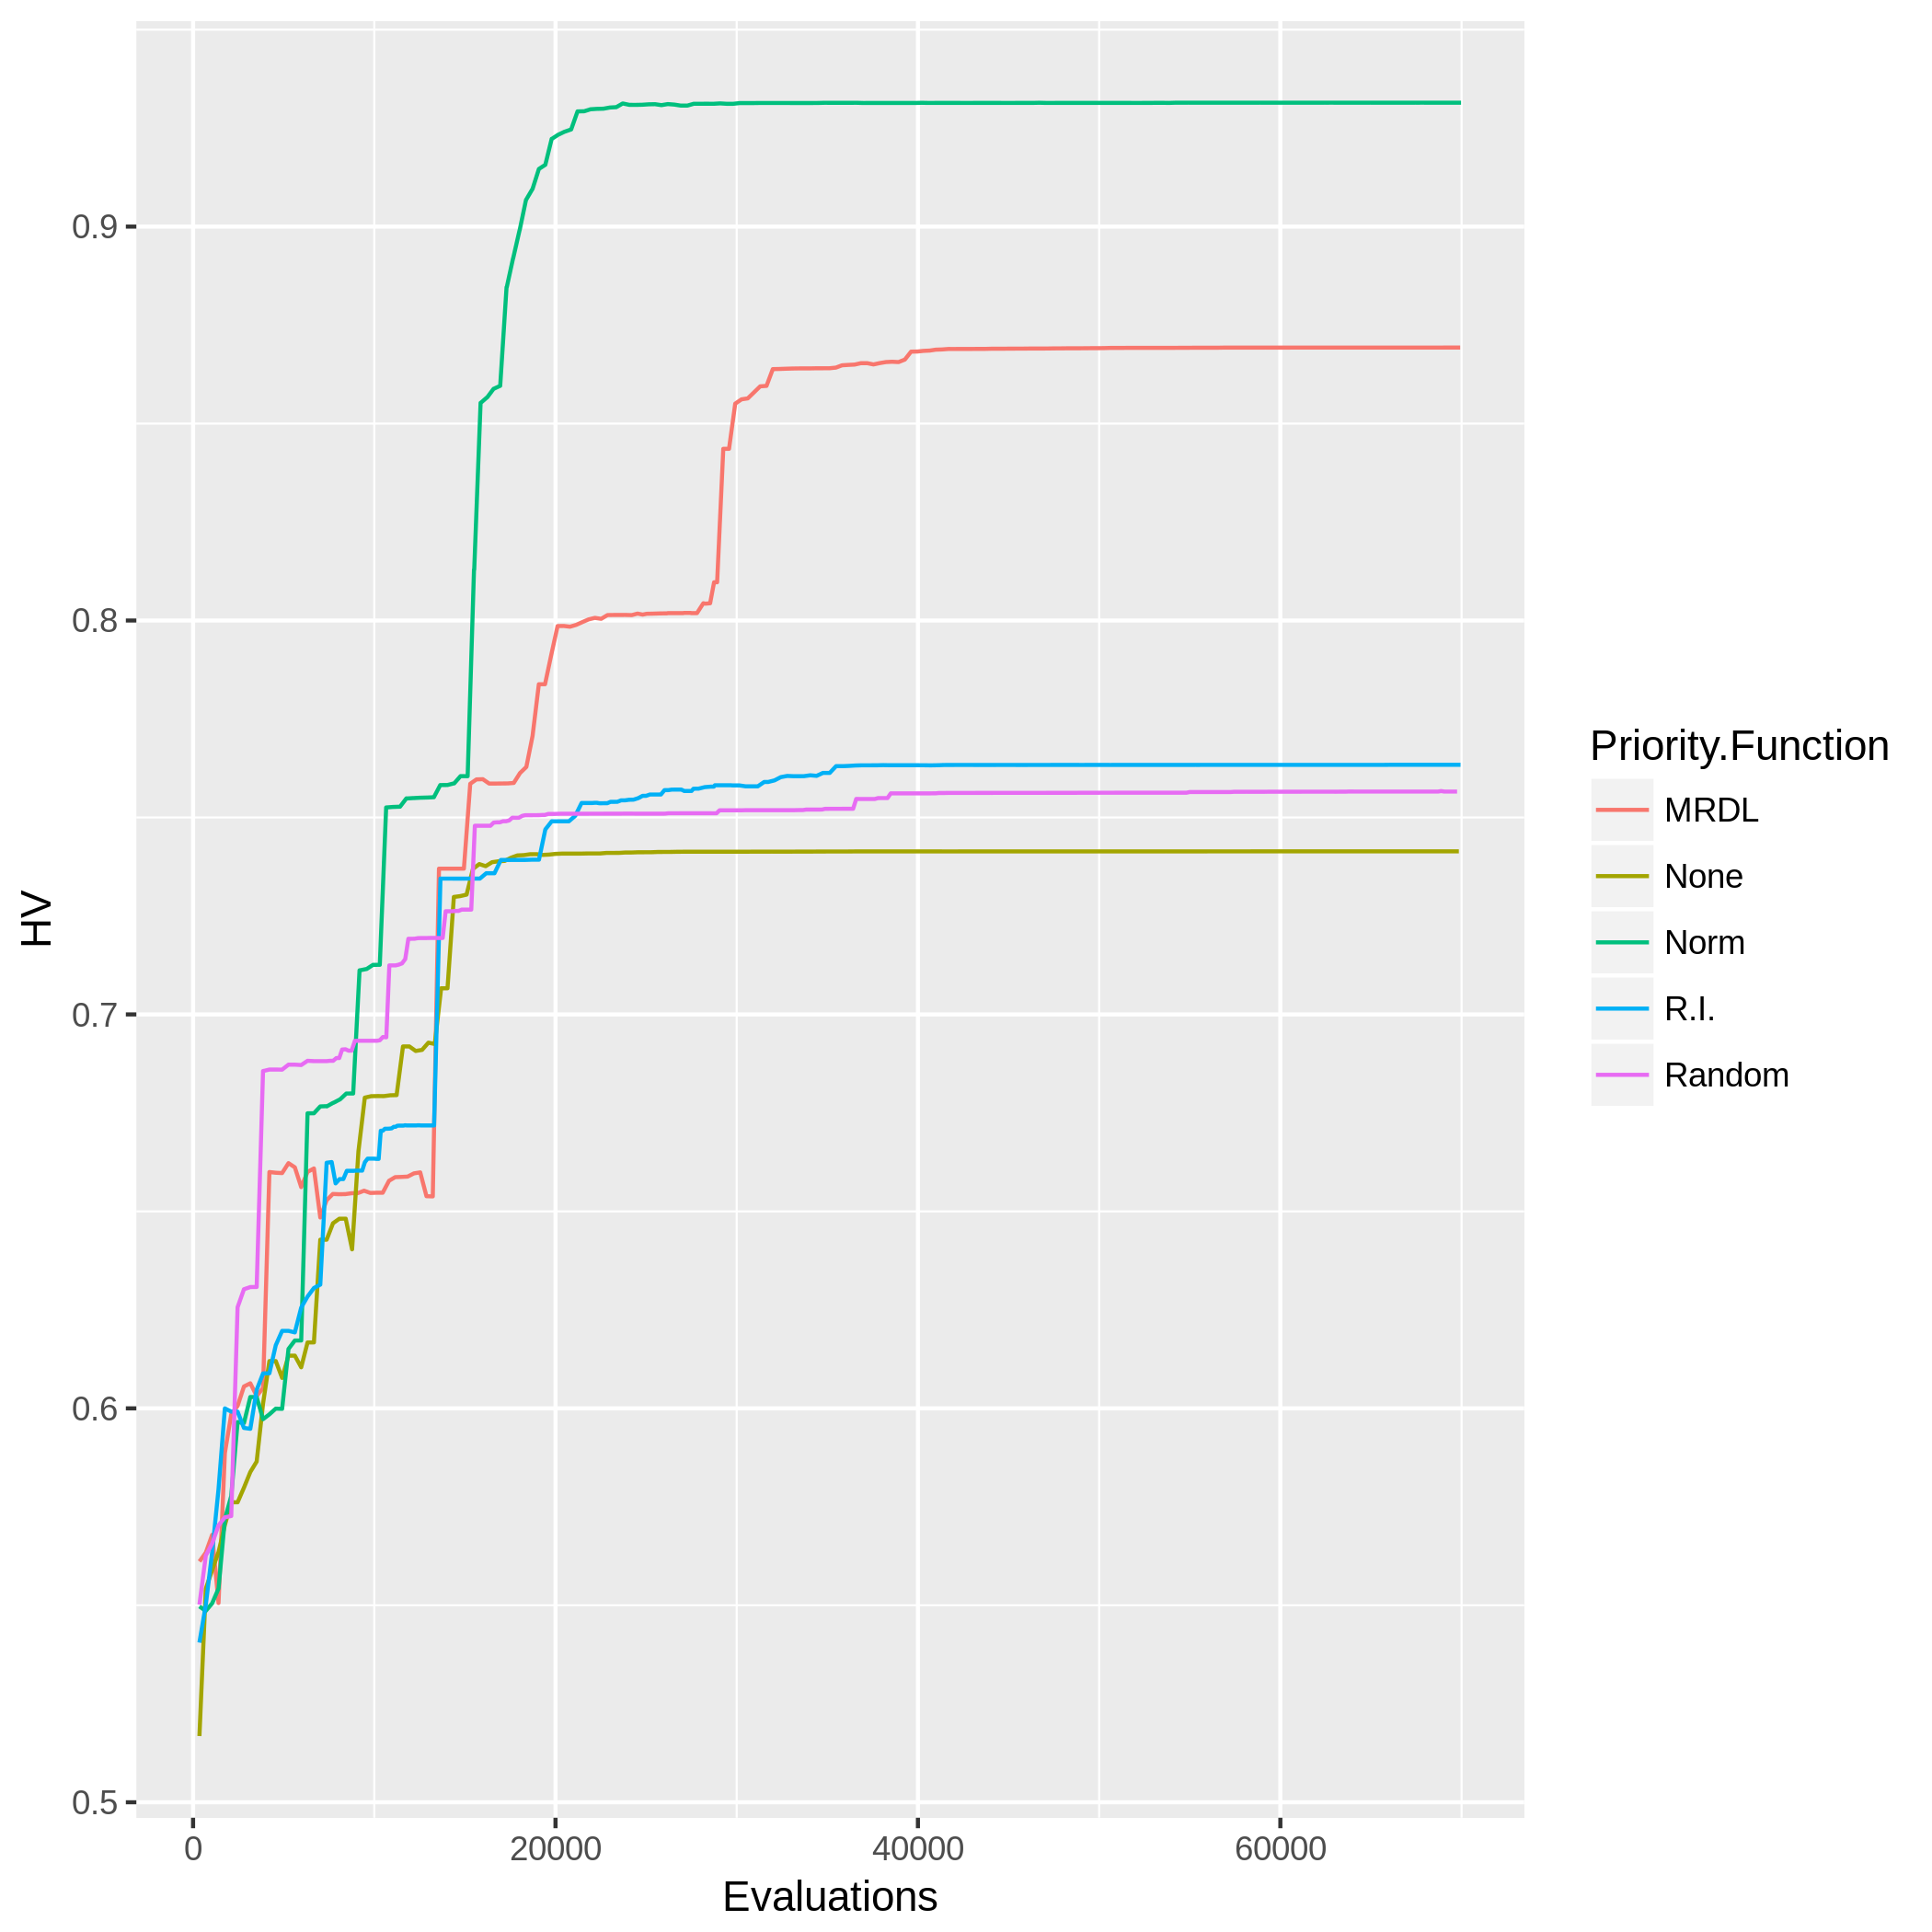
\includegraphics[width=1\textwidth, height=1\textwidth]{images/moonhv_all}
%%		\caption{Evolution of the HV on the Lunar Landing}
%%	\end{subfigure}
%	\caption{SBX crossover - ($\lambda, \lambda$) scheme.}
%	\label{moon}
%\end{figure*}



%\begin{table*}[!t]
%	\begin{tabular}{llllll}
%		\cline{6-6}
%		\hline
%		\rowcolor[gray]{.7} \multicolumn{1}{|l|}{Priority Function:}         & \multicolumn{1}{l|}{None} & \multicolumn{1}{l|}{MRDL} & \multicolumn{1}{l|}{Norm} & \multicolumn{1}{l|}{R.I.} & \multicolumn{1}{l|}{Random} \\ \hline \hline  \hline
%		\multicolumn{1}{|l|}{Lunar (Non-dominated (\%))}           & \multicolumn{1}{l}{0.69 (0.23)} & \multicolumn{1}{l}{0.87 (0.18)} & \multicolumn{1}{l}{0.83 (0.18)} & 0.69 (0.16)             &\multicolumn{1}{l|} {0.44 (0.16)} \\ \hline \hline \hline
%%		\multicolumn{1}{|l|}{Lunar (Time (seconds))}           & \multicolumn{1}{l}{32 (0.92)} & \multicolumn{1}{l}{39 (11.02)} & \multicolumn{1}{l}{46 (23.34)} & 2 (7.75)             &\multicolumn{1}{l|} {52 (0.86)} \\ \hline \hline
%		\rowcolor[gray]{.95} \multicolumn{1}{|l|}{UF1 (Non-dominated (\%))}              & \multicolumn{1}{l}{0.28 (0.03)} & \multicolumn{1}{l}{0.29 (0.05)} & \multicolumn{1}{l}{0.94 (0.10)} & 0.47 (0.09)             &\multicolumn{1}{l|} {0.68 (0.06)} \\ \hline
%%		\rowcolor[gray]{.95} \multicolumn{1}{|l|}{UF1 (Time (seconds))}              & \multicolumn{1}{l}{28 (2.36)} & \multicolumn{1}{l}{46 (2.16)} & \multicolumn{1}{l}{1 (0.60)} & 37 (3.05)            &\multicolumn{1}{l|} {34 (2.87)} \\ \hline \hline
%		\multicolumn{1}{|l|}{UF2 (Non-dominated (\%))}           & \multicolumn{1}{l}{0.34 (0.04)} & \multicolumn{1}{l}{0.34 (0.05)} & \multicolumn{1}{l}{0.96 (0.05)} & 0.61 (0.16)             &\multicolumn{1}{l|} {0.81 (0.06)} \\ \hline
%%		\multicolumn{1}{|l|}{UF2 (Time (seconds))}           & \multicolumn{1}{l}{24 (0)} & \multicolumn{1}{l}{41 (0.59)} & \multicolumn{1}{l}{1 (0.00)} & 34 (1.47)             &\multicolumn{1}{l|} {31 (0.00)} \\ \hline \hline
%		\rowcolor[gray]{.95} \multicolumn{1}{|l|}{UF3 (Non-dominated (\%))}              & \multicolumn{1}{l}{0.22 (0.03)} & \multicolumn{1}{l}{0.24 (0.03)} & \multicolumn{1}{l}{0.78 (0.13)} & 0.44 (0.15)            &\multicolumn{1}{l|} {0.59 (0.07)} \\ \hline
%%		\rowcolor[gray]{.95} \multicolumn{1}{|l|}{UF3 (Time (seconds))}              & \multicolumn{1}{l}{25 (0.22)} & \multicolumn{1}{l}{43 (1.55)} & \multicolumn{1}{l}{1 (0.60)} & 55 (2.09)           &\multicolumn{1}{l|} {31 (0.00)} \\ \hline \hline
%		\multicolumn{1}{|l|}{UF4 (Non-dominated (\%))}           & \multicolumn{1}{l}{0.58 (0.05)} & \multicolumn{1}{l}{0.60 (0.04)} & \multicolumn{1}{l}{0.90 (0.08)} & 0.75 (0.06)             &\multicolumn{1}{l|} {0.82 (0.04)} \\ \hline
%%		\multicolumn{1}{|l|}{UF4 (Time (seconds))}           & \multicolumn{1}{l}{24 (0.00)} & \multicolumn{1}{l}{41 (0.00)} & \multicolumn{1}{l}{1 (0.00)} & 34 (1.56)             &\multicolumn{1}{l|} {31 (0.22)} \\ \hline \hline
%		\rowcolor[gray]{.95} \multicolumn{1}{|l|}{UF5 (Non-dominated (\%))}              & \multicolumn{1}{l}{0.21 (0.03)} & \multicolumn{1}{l}{0.26 (0.04)} & \multicolumn{1}{l}{0.96 (0.03)} & 0.69 (0.13)             &\multicolumn{1}{l|} {0.71 (0.08)} \\ \hline
%%		\rowcolor[gray]{.95} \multicolumn{1}{|l|}{UF5 (Time (seconds))}              & \multicolumn{1}{l}{24 (0.22)} & \multicolumn{1}{l}{41 (0.60)} & \multicolumn{1}{l}{2 (0.44)} & 33 (0.54)             &\multicolumn{1}{l|} {31 (0.22)} \\ \hline \hline
%		\multicolumn{1}{|l|}{UF6 (Non-dominated (\%))}           & \multicolumn{1}{l}{0.27 (0.03)} & \multicolumn{1}{l}{0.27 (0.03)} & \multicolumn{1}{l}{0.95 (0.08)} & 0.45 (0.07)             &\multicolumn{1}{l|} {0.61 (0.07)} \\ \hline
%%		\multicolumn{1}{|l|}{UF6 (Time (seconds))}           & \multicolumn{1}{l}{24 (0.36)} & \multicolumn{1}{l}{41 (0.79)} & \multicolumn{1}{l}{1 (0.00)} & 33 (0.51)             &\multicolumn{1}{l|} {31 (0.00)} \\ \hline \hline
%		\rowcolor[gray]{.95} \multicolumn{1}{|l|}{UF7 (Non-dominated (\%))}              & \multicolumn{1}{l}{0.38 (0.06)} & \multicolumn{1}{l}{0.37 (0.05)} & \multicolumn{1}{l}{0.96 (0.03)} & 0.57 (0.11)             &\multicolumn{1}{l|} {0.80 (0.04)} \\ \hline
%%		\rowcolor[gray]{.95} \multicolumn{1}{|l|}{UF7 (Time (seconds))}              & \multicolumn{1}{l}{24 (0.30)} & \multicolumn{1}{l}{42 (0.38)} & \multicolumn{1}{l}{1 (0.46)} & 34 (0.90)             &\multicolumn{1}{l|} {31 (0.30)} \\ \hline \hline
%		\multicolumn{1}{|l|}{UF8 (Non-dominated (\%))}           & \multicolumn{1}{l}{0.40 (0.03)} & \multicolumn{1}{l}{0.39 (0.03)} & \multicolumn{1}{l}{0.70 (0.06)} & 0.67 (0.07)             &\multicolumn{1}{l|} {0.63 (0.03)} \\ \hline
%%		\multicolumn{1}{|l|}{UF8 (Time (seconds))}           & \multicolumn{1}{l}{24 (0.00)} & \multicolumn{1}{l}{39 (0.58)} & \multicolumn{1}{l}{1 (0.00)} & 51 (2.23)             &\multicolumn{1}{l|} {31 (0.30)} \\ \hline \hline
%		\rowcolor[gray]{.95} \multicolumn{1}{|l|}{UF9 (Non-dominated (\%))}              & \multicolumn{1}{l}{0.32 (0.03)} & \multicolumn{1}{l}{0.33 (0.03)} & \multicolumn{1}{l}{0.52 (0.03)} & 0.49 (0.04)             &\multicolumn{1}{l|} {0.48 (0.03)} \\ \hline
%%		\rowcolor[gray]{.95} \multicolumn{1}{|l|}{UF9 (Time (seconds))}              & \multicolumn{1}{l}{25 (0.50)} & \multicolumn{1}{l}{23 (4.59)} & \multicolumn{1}{l}{1 (27.84)} & 47 (2.75)             &\multicolumn{1}{l|} {32 (0.48)} \\ \hline \hline
%		\multicolumn{1}{|l|}{UF10 (Non-dominated (\%))}           & \multicolumn{1}{l}{0.43 (0.04)} & \multicolumn{1}{l}{0.46 (0.05)} & \multicolumn{1}{l}{0.75 (0.05)} & 0.68 (0.08)             &\multicolumn{1}{l|} {0.73 (0.06)} \\ \hline \hline \hline
%%		\multicolumn{1}{|l|}{UF10 (Time (seconds))}           & \multicolumn{1}{l}{25 (0.51)} & \multicolumn{1}{l}{38 (1.83)} & \multicolumn{1}{l}{1 (0.00)} & 47 (3.51)             &\multicolumn{1}{l|} {32 (0.30)} \\ \hline \hline
%		\rowcolor[gray]{.95} \multicolumn{1}{|l|}{DTLZ1 (Non-dominated (\%))}              & \multicolumn{1}{l}{0.05 (0.01)} & \multicolumn{1}{l}{0.07 (0.01)} & \multicolumn{1}{l}{0.98 (0.06)} & 0.62 (0.17)             &\multicolumn{1}{l|} {0.68 (0.13)} \\ \hline
%%		\rowcolor[gray]{.95} \multicolumn{1}{|l|}{DTLZ1 (Time (seconds))}              & \multicolumn{1}{l}{25 (0.90)} & \multicolumn{1}{l}{41 (1.16)} & \multicolumn{1}{l}{2 (0.00)} & 36 (10.19)             &\multicolumn{1}{l|} {32 (0.00)} \\ \hline \hline
%		\multicolumn{1}{|l|}{DTLZ2 (Non-dominated (\%))}           & \multicolumn{1}{l}{0.18 (0.03)} & \multicolumn{1}{l}{0.25 (0.03)} & \multicolumn{1}{l}{0.96 (0.05)} & 0.73 (2.93)             &\multicolumn{1}{l|} {0.84 (0.07)} \\ \hline
%%		\multicolumn{1}{|l|}{DTLZ2 (Time (seconds))}           & \multicolumn{1}{l}{25 (0.30)} & \multicolumn{1}{l}{41 (0.54)} & \multicolumn{1}{l}{1 (12.66)} & 40 (2.93)             &\multicolumn{1}{l|} {32 (0.60)} \\
%		\rowcolor[gray]{.95} \multicolumn{1}{|l|}{DTLZ3 (Non-dominated (\%))}              & \multicolumn{1}{l}{0.04 (0.02)} & \multicolumn{1}{l}{0.04 (0.02)} & \multicolumn{1}{l}{0.99 (0.05)} & 0.32 (0.17)             &\multicolumn{1}{l|} {0.44 (0.18)} \\ \hline
%%		\rowcolor[gray]{.95} \multicolumn{1}{|l|}{DTLZ3 (Time (seconds))}              & \multicolumn{1}{l}{25 (0.22)} & \multicolumn{1}{l}{40 (0.78)} & \multicolumn{1}{l}{2 (0.51)} & 32 (3.09)             &\multicolumn{1}{l|} {32 (0.22)} \\ \hline \hline
%		\multicolumn{1}{|l|}{DTLZ4 (Non-dominated (\%))}           & \multicolumn{1}{l}{0.11 (0.03)} & \multicolumn{1}{l}{0.13 (0.03)} & \multicolumn{1}{l}{0.96 (0.03)} & 0.7 (0.24)             &\multicolumn{1}{l|} {0.63 (0.13)} \\ \hline
%%		\multicolumn{1}{|l|}{DTLZ4 (Time (seconds))}           & \multicolumn{1}{l}{26 (0.36)} & \multicolumn{1}{l}{43 (1.01)} & \multicolumn{1}{l}{1 (0.00)} & 47 (5.94)             &\multicolumn{1}{l|} {33 (0.68)} \\ \hline \hline
%		\rowcolor[gray]{.95} \multicolumn{1}{|l|}{DTLZ5 (Non-dominated (\%))}              & \multicolumn{1}{l}{0.18 (0.02)} & \multicolumn{1}{l}{0.24 (0.03)} & \multicolumn{1}{l}{0.96 (0.05)} & 0.75 (0.14)             &\multicolumn{1}{l|} {0.84 (0.06)} \\ \hline
%%		\rowcolor[gray]{.95} \multicolumn{1}{|l|}{DTLZ5 (Time (seconds))}              & \multicolumn{1}{l}{2425 (1.12)} & \multicolumn{1}{l}{38 (0.49)} & \multicolumn{1}{l}{1 (0.00)} & 39 (2.83)             &\multicolumn{1}{l|} {30 (0.26)} \\ \hline \hline
%		\multicolumn{1}{|l|}{DTLZ6 (Non-dominated (\%))}           & \multicolumn{1}{l}{0.04 (0.02)} & \multicolumn{1}{l}{0.03 (0.02)} & \multicolumn{1}{l}{1.00 (0.00)} & 0.95 (0.33)             &\multicolumn{1}{l|} {0.56 (0.25)} \\ \hline
%%		\multicolumn{1}{|l|}{DTLZ6 (Time (seconds))}           & \multicolumn{1}{l}{25 (0.22)} & \multicolumn{1}{l}{38 (0.48)} & \multicolumn{1}{l}{1 (0.51)} & 33 (0.87)             &\multicolumn{1}{l|} {31 (0.30)} \\ \hline \hline
%		\rowcolor[gray]{.95} \multicolumn{1}{|l|}{DTLZ7 (Non-dominated (\%))}              & \multicolumn{1}{l}{0.13 (0.05)} & \multicolumn{1}{l}{0.13 (0.04)} & \multicolumn{1}{l}{0.97 (0.08)} & 0.66 (0.13)             &\multicolumn{1}{l|} {0.63 (0.08)} \\ \hline
%%		\rowcolor[gray]{.95} \multicolumn{1}{|l|}{DTLZ7 (Time (seconds))}              & \multicolumn{1}{l}{25 (0.22)} & \multicolumn{1}{l}{2 (0.00)} & \multicolumn{1}{l}{1 (0.00)} & 41 (1.47)             &\multicolumn{1}{l|} {30 (0.22)} \\ \hline
%	\end{tabular}
%	\caption{Percentage of the median values and the standard deviation in parenthesis of non-dominated solutions. None is the MOEA/D-DE with no priority function.}
%	\label{minor_results}
%\end{table*}

%\subsubsection{UF benchmark functions}


Figure~\ref{HVS} shows box-plot that exemplify the results found in the UF benchmark and DTLZ functions as well as the Lunar Landing problem in terms of the HV values. Figure~\ref{IGDS} does the same but in terms of the IGD values, but only to the artificial benchmarks. Finally, Figure~\ref{PFs} illustrates the PF approximation for the DTLZ4 found by all priority functions and without it.

In all these Figures, we can see that, in general, using resource allocation performs better than not using resource allocation. The Tables~\ref{table_hv_igd} and~\ref{minor_results} reinforces these results. The priority functions R.I., Norm, and Random achieve similar results in terms of HV values. These results are indicated by the box-plots~\ref{HVS}, the Table~\ref{table_hv_igd}, the approximation to the PF~\ref{PFs}, and the Pairwise Wilcoxon Rank Sum Tests~\ref{statistics}. We ask ourselves if the fact that Random performed as well as Norm and RI in HV indicates that there is still space for finding more appropriate priority functions. For IGD values, the same trend is confirmed, however, there is statistically significance difference between the results of Norm and R.I~\ref{statistics}. On the Lunar Landing Problem, all strategies found similar Hypervolume results (Table~\ref{table_hv_igd}). 

Now we move to the results in the Table~\ref{table_hv_igd}. It shows the results for every priority function measured by HV and IGD.  First we discuss the results for the UF functions, then the results for the DTLZ functions and lastly the results for the Lunar Problem. 

In the UF functions and considering the results of the HV metric, Norm as priority function had few good results. with the best median in UF3 and UF9. The R.I. had the higher median in five functions. Surprisingly, the Random priority function got the higher median in the UF2, UF4 and UF6. When considering IGD the Norm had the best median in UF3, UF4, UF5, UF7, UF8 and UF9 functions. The R.I. had the highest median in the 4 functions. Again, Random surprised us, being the best in UF2 and Uf4. In both metrics, MRDL had slightly better results than MOEA/D-DE.

Now, for the DTLZ set and first considering HV values, Norm as priority function lead to several good results in median in DTLZ2, DTLZ6 and DTLZ7 functions. R.I. performed as the best algorithm in terms of median of HV values also in 3 functions. Reinforcing our surprise, the Random priority function got the higher median in the DTLZ1, DTLZ2, DTLZ3 and DTLZ5 functions. For the values of the IGD, Norm had the best medians in the functions: DTLZ2, DTLZ5 and DTLZ6, again with the same number of best results as R.I. Here, Only in the DTLZ1 Random had the highest values.

On the Lunar Landing Problem, the best priority function in terms of median HV values is the MRDL. However, as commented above, the results are all similar. 

%That said, the best priority function in terms of median values is the MRDL.

% for the artificial benchmarks MRDL is slightly better than MOEA/D-DE, considering both HV and IGD values. Norm, R.I. and Random perform the best. On the other hand, MRDL performs the best in the Lunar problem, followed by R.I., Norm and lastly by MOEA/D-DE.


%Figure~\ref{HVS} shows box-plot that exemplify the results found in the UF benchmark and DTLZ functions as well as the Lunar Landing problem in terms of the HV values. Figure~\ref{IGDS} does the same but in terms of the IGD values, but only to the artificial benchmarks. In them we can see that for the artificial benchmarks MRDL is slightly better than MOEA/D-DE, considering both HV and IGD values. Norm, R.I. and Random perform the best. On the other hand, MRDL performs the best in the Lunar problem, followed by R.I., Norm and lastly by MOEA/D-DE.


%Figure~\ref{PFs} illustrates the PF approximation for the DTLZ4 found by all priority functions and without it. In agreement with the results given by the HV and IGD (Table~\ref{table_hv_igd}), both Norm and R.I. approximate well the PF. On the other hand it is clear that MRDL did not lead to a better approximation of the PF when compared to the one of MOEA/D-DE. More results can be found at the supplementary materials.
%
%\subsection{HV Results}
%
%Table~\ref{table_hv_igd} shows the results for every priority function measured by HV in the first part. First we discuss the results for the UF functions, then the results for the DTLZ functions and lastly the results for the Lunar Problem. Norm as priority function had few good results, with  the best median in UF3 and UF9. In UF3, there is no statistical significant difference for the R.I. while in UF9, there is no statistical significant difference for the Random. The R.I. had the higher median in five functions. Only in UF8 results there exists a statistical significant difference to the other priority functions.  In UF1, UF5 and UF7 statistical significant difference to the results of the Random. Surprisingly, the Random priority function got the higher median in the UF2 (with no statistical difference to R.I.), UF4 (with no statistical difference to R.I. or Norm) and UF6 (with no statistical difference to R.I.). MRDL had slightly better results than MOEA/D-DE, however only in UF3 and UF8 the results had statistical significance.
%
%Now, we discuss to the results on the DTLZ functions. Norm as priority function lead to several good results in median with the best median in the DTLZ2 (no statistical difference to Random), DTLZ5 (no statistical difference to Random or R.I) , DTLZ6 and DTLZ7 (no statistical difference to R.I.) cases. Only in the DTLZ6 the difference in the results had statistical significance. R.I. performed as the best algorithm in terms of median of HV values only in the DTLZ4 (without any significant difference to Random or Norm). Reinforcing our surprise, the Random priority function got the higher median in the DTLZ1 (with no statistical difference to Norm or R.I.), DTLZ2 (with no statistical difference to R.I.), DTLZ3 and DTLZ5 functions(both without statistical difference to Norm or R.I.), with its median being always higher that the one from MRDL.
%
%On the Lunar Problem, the best priority function is the MRDL, the only one with statistical difference to MOEA/D-DE. However, the results of this priority function have no statistical difference to the other priority functions.
%
%\subsection{IGD Results}
%
%We again start with the UF results and then move to the DTLZ results. In the Table~\ref{table_hv_igd} (second part) we verify that the Norm had the best median in 6 functions, being statistically different to all others in the UF3, UF5, UF7 and UF9 functions. In the UF4, the result of the Norm are not statistically different from the R.I. or the Random. In UF8 the results of the Norm not statistically different from the Random. The R.I. had the highest median in the UF1, UF4, UF6 and UF10 functions. The results of UF1 and UF4 are not statistically different from the R.I. or the Random. In UF6 the results are not statistically different from the Random while on the UF10, there is no statistical different to the results of the Norm. Norm had the best results in UF2 having the same median as Norm and R.I., with a lower standard deviation. Again, MRDL had slightly better results than MOEA/D-DE, however only in UF3 and UF8 the results had statistical significance.
%
%Moving to the DTLZ results, we verify that the Norm had the best median in 3 functions, DTLZ2, DTLZ5 (with no statistical difference to Random or R.I.) and DTLZ67 (with no statistical difference to Random). In the DTLZ2 the results had statistical difference. The R.I. perform the best in the DTLZ3 (with no statistical difference to Norm or Random), DTLZ5 and DTLZ7(both with no statistical difference to Norm). Only in the DTLZ1  Random had the highest values(with no statistical difference to Norm or R.I.).



\subsection{Rate - Non-dominated and Feasible Solutions}

%%% Dominance and feasibility
% Another difference that we see among the Resource Allocation strategies is found in the proportion of non dominated and feasible solutions. For the Benchmark problems, the Norm Strategy achieved a very high fraction of non-dominated solutions in the final solution set. In the Lunar Landing problem, the Norm strategy achieved a higher proportion of feasible solutions than the other resource allocation strategies.It is always the fastest, mean time of the median of every function: 1.17; standard deviation (sd): 2.46. The MRDL priority function improved a little the rate of non-dominated solutions, at the cost of a longer execution time (mean time of the median of every function: 37.53; sd: 1.03). The same behavior (better rate of non-dominated solutions, more cost in time) is found in the R.I.(mean time of the median of every function: 39; sd: 5.14) and Random results (mean time of the median of every function: 31.47; sd: 0.41).

Another difference that we see among the Resource Allocation strategies is found in the proportion of non dominated and feasible solutions. The results on the Table~\ref{minor_results} indicate that the Norm strategy leads to a very high rate of non-dominated solutions in the final solution set. It is always the fastest, mean time of the median of every function: 1.17; standard deviation (sd): 2.46. The MRDL priority function improved a little the rate of non-dominated solutions, at the cost of a longer execution time (mean time of the median of every function: 37.53; sd: 1.03). The same behavior (better rate of non-dominated solutions, more cost in time) is found in the R.I.(mean time of the median of every function: 39; sd: 5.14) and Random results (mean time of the median of every function: 31.47; sd: 0.41).

On the Lunar Landing problem, Norm had the highest rate of feasible solutions, but had the second best rate of non-dominated solutions, surpassed by R.I., both were the slowest, Norm: mean time of 6.81 with sd of 0.40; R.I.: mean time of 6.95 and sd of 1.02. MRDL found less feasible solutions than any other strategy (besides the random), but it was the fastest, mean time of 4.95 and sd of 0.21.


% lunar landingOn the other hand, it exceed the rate of non-dominated solutions of the MOEA/D-DE and it was the fastest, mean time of 4.95 and sd of 0.21. MOEA/D-DE had mean time of 6.67 and sd of 1.98.  Both priority functions were the slowest, Norm: mean time of 6.81 with sd of 0.40; R.I.: mean time of 6.95 and sd of 1.02.



% Figures~\ref{evolution_hv} and~\ref{evolution_igd} show how the values of the HV and IGD evolve over the iteractions of the algorithms. For the UF3 function the results caught our attention. First, it seems that more evaluations are need to a convergence of the values. Second, for the HV values the priority functions relative improvement and Norm made a "jump" over 30000 and 60000 evaluations, improving fast the HV metric values. Also at the end fo the evaluations, there is a strange regressive peak of the HV and IGD values of the Norm. That said, in most cases the values of HV and IGD converged by the end of the number evaluations (70000).

%\subsubsection{DTLZ benchmark functions}





%\subsubsection{Lunar Landing Problem}


%Figure~\ref{moon} show box-plot the results found in the Lunar Landing benchmark problem in terms of the HV values. Both priority functions related to diversity, MRDL and Norm, improved a lot the performance of the MOEA/D-DE. On the other hand, R.I. lead to a diminish of the standard deviation, with just a slight improvement on the performance. % Figure~\ref{moon} (b) show how the values of the HV evolve over the iteractions of the algorithms. All of the variants had converged around 20000 evaluations, with the exception of the MRDL (it converged with 40000). All used around half or less of the total number evaluations (70000) to converge.





\subsection{Resource Allocation}

%%% Figure 4 shows how the different strategies are allocating results for functions UF9 and DTLZ4. It is interesting to observe that RI and Norm assign similar priorities to the same subproblems in the DTLZ4. But they find opposite priorities to subproblems on the UF9 function.


Figure~\ref{RAs} illustrates the amount resource allocated by Norm, R.I. and MRDL to every subproblem on UF3 and DTLZ4 problems. We show images from the UF9 and DTLZ4 functions due to space limitations, but similar images for the other problems are available in the supplementary materials. We exclude the visuals from MOEA/D-DE since it give the same amount of resource to every problem (200) and of the Random, since it is completely noisy.

It is clear from this Figure~\ref{RAs} that, during the execution of the algorithm, the resource allocate to each subproblem is different. This behavior is different given priority functions, illustrating that every priority function allocates different amount of resource given their characteristics. It is also important to highlight that each priority function influences the search differently given different MOPs.

It called our attention the results form the priority functions Norm and R.I. in the UF9 function, since it appears to be that they prioritized subproblems in an opposite way. In the DTLZ4 they appear to prioritize similar subproblems, assigning similar priorities to the same subproblems. The distribution of resource is less abrupt in the case of Norm, however R.I. had better results. MRDL influences weakly the distribution of resource allocation, which might indicate its poor performance. In both cases shown the its distribution got closer to 200 resources per subproblem, the rate of not using any priority function.





%\subsubsection{Non-Dominated Solutions and Execution Time}

\section{Conclusion}

In this paper, we have proposed two new priority functions, related to diversity. One based on the MRDL focus on diversity on the objective space while the Norm focus on diversity on the decision space. We then compared the results with the priority function from the MOEA/D-DRA, R.I. and the MOEA/D-DE variant. 

To summarize the results, using a priority functions that is based on diversity, as the Norm gave very good results in the artificial benchmark functions, even better than the R.I. a common priority function from the literature while the MRDL performed the best in the Lunar Landing Problem. Therefore, we suggest exploring priority function based on diversity is a preeminent direction of study that should be further explore. 

Although the MRDL had a good result in the Lunar problem, we expected that MRDL would give the best results in terms of improvement in performance in the artificial benchmarks. The reason might be that this method considers the diversity of a solution against all the population while the two best priority functions consider only the a relationship of the current solution against its parent. More effort should be directed to address the question of why random as priority function performed so well.

From the results on two artificial benchmark functions and one real-world problem, we understand that using priority functions related to diversity is one promising way of finding better results. More studies need to be conducted to understand how diversity really affects the improvement of performance. We also understand that in priority functions improve the performance of MOEA/D-DE in both HV and IGD metrics values as well as at the number of non-dominated solutions.% Finally, we add that using priority function could help to prioritize desired characteristics, as diversity (2-Norm) or convergence towards the PF (R.I.) and maybe some other features.

%There are many other components and variants of MOEA/D and is interesting to combine them with the 2-Norm and MRDL priority functions. Then we can better understand the relationship of priority functions based on diversity with the others components and variants of the MOEA/D framework. How to define more efficient and effective utility functions for different problems is also worth further investigation as well as verify the results of using priority function in others real-world problems.

%It is in our understand that using priority functions in both real-world and artificial benchmarks improve the results of MOEA/D-DE. For all group of functions the performance of MOEA/D-DE, in terms of HV or IGD median values, was always suppressed by at least one variation using priority functions. 

\clearpage

\bibliographystyle{ACM-Reference-Format}
\bibliography{sample} 

\end{document}
